%                                                                 aa.dem
% AA vers. 8.2, LaTeX class for Astronomy & Astrophysics
% demonstration file
%                                                       (c) EDP Sciences
%-----------------------------------------------------------------------
%
%\documentclass[referee]{aa} % for a referee version
%\documentclass[onecolumn]{aa} % for a paper on 1 column  
%\documentclass[longauth]{aa} % for the long lists of affiliations 
%\documentclass[rnote]{aa} % for the research notes
%\documentclass[letter]{aa} % for the letters 
%\documentclass[bibyear]{aa} % if the references are not structured 
% according to the author-year natbib style

%
\documentclass[onecolumn]{aa}  

%
\usepackage{graphicx}
%%%%%%%%%%%%%%%%%%%%%%%%%%%%%%%%%%%%%%%%
\usepackage{txfonts}
\usepackage{amsmath}	% Advanced maths commands
\usepackage{amssymb}	% Extra maths symbols
\usepackage{xspace}
\usepackage{lscape}
\usepackage{color}
\usepackage{longtable}
%\usepackage{url}
%%%%%%%%%%%%%%%%%%%%%%%%%%%%%%%%%%%%%%%%
%\usepackage[options]{hyperref}
% To add links in your PDF file, use the package "hyperref"
% with options according to your LaTeX or PDFLaTeX drivers.
%

\newcommand{\OII}{$\left[\mathrm{O\textrm{\textsc{ii}}}\right]$\xspace}
\newcommand{\OIIll}{$\left[\mathrm{O\textrm{\textsc{ii}}}\right]\,(\lambda\lambda 3729,3726)$\xspace}
\newcommand{\OIII}{$\left[\mathrm{O\textrm{\textsc{iii}}}\right]$\xspace}
\newcommand{\OIIIl}{$\left[\mathrm{O\textrm{\textsc{iii}}}\right]\,(\lambda\lambda 4959,5007)$\xspace}
\newcommand{\OIIIa}{$\left[\mathrm{O\textrm{\textsc{iii}}}\right]\,(\lambda 4959)$\xspace}
\newcommand{\OIIIb}{$\left[\mathrm{O\textrm{\textsc{iii}}}\right]\,(\lambda 5007)$\xspace}
\newcommand{\NeIII}{$\left[\mathrm{Ne\textrm{\textsc{iii}}}\right]$\xspace}
\newcommand{\NII}{$\left[\mathrm{N\textrm{\textsc{ii}}}\right]$\xspace}
\newcommand{\NIIl}{$\left[\mathrm{N\textrm{\textsc{ii}}}\right]\,(\lambda 6584)$\xspace}
\newcommand{\SII}{$\left[\mathrm{S\textrm{\textsc{ii}}}\right]$\xspace}
\newcommand{\SIIl}{$\left[\mathrm{S\textrm{\textsc{ii}}}\right]\,(\lambda\lambda 6716,6731)$\xspace}
\newcommand{\SIIa}{$\left[\mathrm{S\textrm{\textsc{ii}}}\right]\,(\lambda 6716)$\xspace}
\newcommand{\SIIb}{$\left[\mathrm{S\textrm{\textsc{ii}}}\right]\,(\lambda 6731)$\xspace}
\newcommand{\Ha}{H${\alpha}$\xspace}
\newcommand{\Hb}{H${\beta}$\xspace}
\newcommand{\Hbl}{H${\beta}\,(\lambda 4861)$\xspace}
\newcommand{\Hd}{H${\delta}$\xspace}
\newcommand{\Hg}{H${\gamma}$\xspace}
\newcommand{\Ly}{Ly${\alpha}$\xspace}
\newcommand{\uflux}[0]{${\rm erg \cdot s^{-1} \cdot cm^{-2}}$\xspace}
\newcommand{\ufluxA}[0]{${\rm erg \cdot s^{-1} \cdot cm^{-2} \mathring{A}^{-1}}$\xspace}
\newcommand{\HII}{$\mathrm{H\textrm{\textsc{ii}}}$\xspace}

\begin{document} 

\title{Stellar population properties for 2 million galaxies from SDSS DR14 and DEEP2 DR4 from full spectral fitting}
\titlerunning{Stellar populations in SDSS and DEEP2}
\author{
Johan Comparat\inst{1} 
\and
Claudia Maraston\inst{2} 
\and
Daniel Goddard\inst{2}
\and
Violeta Gonzalez-Perez\inst{2} 
\and
Jianhui Lian\inst{2}
\and
Sofia Meneses-Goytia\inst{2}
\and
Daniel Thomas\inst{2} 
\and
Joel R. Brownstein\inst{3}  
\and
Rita Tojeiro\inst{4} 
\and
Alexis Finoguenov\inst{1,9} 
\and
Andrea Merloni\inst{1} 
\and
Francisco Prada\inst{5}
\and
Mara Salvato\inst{1} 
\and
Guangtun B. Zhu\inst{6}
\and
Hu Zou\inst{7}
\and
Jonathan Brinkmann\inst{8}
}
\institute{
Max-Planck-Institut f\"{u}r extraterrestrische Physik (MPE), Giessenbachstrasse 1, D-85748 Garching bei München, Germany\\
\email{comparat@mpe.mpg.de}
\and
Institute of Cosmology and Gravitation, University of Portsmouth, Portsmouth, PO1 3FX, UK\\
\and
Department of Physics and Astronomy, University of Utah, 115 S. 1400 E., Salt Lake City, UT 84112, USA \\
\and
School of Physics and Astronomy, North Haugh, St. Andrews KY16 9SS, UK \\
\and
Instituto de Astrof\'{\i}sica de Andaluc\'{\i}a (CSIC), Glorieta de la Astronom\'{\i}a, E-18080 Granada, Spain \\
\and
Center for Astrophysical Sciences, Department of Physics and Astronomy, Johns Hopkins University, 3400 North Charles Street, Baltimore, MD 21218, USA\\ 
\and 
Key Laboratory of Optical Astronomy, National Astronomical Observatories, Chinese Academy of Sciences, Beijing 100012, China\\
\and 
Apache Point Observatory, P.O. Box 59, Sunspot, NM 88349\\
\and
Department of Physics, University of Helsinki, Gustaf H\"allstr\"omin katu 2a, FI-00014 Helsinki, Finland\\
}

% These dates will be filled out by the publisher
\date{Received Nov 16, 2017}

\abstract
{}
{We determine the stellar population properties - age, metallicity, dust reddening, stellar mass and the star formation history - for all spectra classified as galaxies that were published by the Sloan Digital Sky Survey (SDSS data release 14) and by the DEEP2 (data release 4) galaxy surveys.}
{We perform full spectral fitting on individual spectra, making use of high spectral resolution stellar population models. Calculations are carried out for several choices of the model input, including three stellar initial mass functions and three input stellar libraries to the models. We study the accuracy of parameter derivation, in particular the stellar mass, as a function of the signal-to-noise of the galaxy spectra. We find that signal to noise ratio per pixel around 20 (5) allow a statistical accuracy on $\log_{10}(M^{*}/M_{\odot})$ of 0.2 (0.4) dex, for the Chabrier IMF.}
{%We obtain the galaxy stellar mass function probed by SDSS, eBOSS and DEEP2 for galaxies with $0.2<z<0.8$. 
For the first time, we study DEEP2 galaxies selected by their \OII luminosity in the redshift range $0.83<z<1.03$, finding that they have stellar masses with a flat number density in the range $10^9<M/M_{\odot}<10^{11.5}$. 
We publish all catalogs of properties as well as model spectra of the continuum for these galaxies as a value added catalog of the fourteenth data release of the SDSS. This catalog is about twice as large as its predecessors (DR12) and will aid a variety of studies on galaxy evolution and cosmology.}
{}

\keywords{galaxy evolution - stellar population model - galaxy surveys }
\maketitle

% \section{COMMENTS}
% \begin{itemize}
%\item  I agree that it’s plausible that ELODIE gives higher errors because of the smaller wavelength range. Has this been shown somewhere (by restricting other libraries to the same range)? If so, give details.
%\item  About EBV : Obtain HPF EBV values for a different wavelength range say 4000 to 5000 A. Force Calzetti law on firefly. 
%\item  Need to asses how the wavelength coverage of the spectra matters.
%\item  As your main point is the addition of low s/n estimates, it makes sense to show the difference they make in the sampling of the galaxy stellar mass functions. Also, it would be nice to draw conclusions from your sfr-based mass functions, and compare to previous results.
%\end{itemize}
%%%%%%%%%%%%%%%%%%%%%%%%%%%%%%%%%%%%%%%%%%%%%%%%%%
%%%%%%%%%%%%%%%%% BODY OF PAPER %%%%%%%%%%%%%%%%%%
\section{Introduction}
\label{sec:introduction}

In the current paradigm of galaxy evolution, structures and galaxies form hierarchically: larger halos are formed by the coalescence of smaller progenitors. 
From a macroscopic or thermodynamical point of view, galaxies are typically described as systems composed of the following tightly interacting sub-systems: the dark matter halo, the central black hole, the stars, the cold gas, the hot gas and the dust. 
In addition, the galaxy interacts with its surroundings, the intergalactic medium, where it ejects gas or from where it aggregates matter. 
A galaxy in this model is characterized by the mass of each of its components and the share of mass constituted by elements heavier than hydrogen. 
The visible component of galaxies is approximated as a tri-phased system made of stars, inter-stellar medium and circum-galactic medium. This system is driven by the stellar activity; e.g. star formation rate, supernovae rate, the activity of the central active part of the galaxy; that induce gas movements: winds, accretion and expulsion \citep{mo2010book}. What stars populate galaxies is thus a central question in galaxy evolution. 

The method to infer a galaxy stellar properties (e.g. stellar ages, chemical composition, dust effects, the star formation history and the stellar mass) consists in fitting models to the observed spectral energy distribution. 
There exist many variants of this method. 
Variations occurs in all dimensions of the problem: the models of the stellar population, the wavelength covered by observations or by models, the fitting method to compare models and data (e.g. statistics, priors, etc.). 
% Stellar mass function literature 
% \citet{moustakas2013}
% \citet{Ilbert2013SMF}
In this study we use the \citet{Maraston_2011} (M11 hereafter) stellar population models together with the \textsc{firefly} fitting routine \citep{Wilkinson_2015,Goddard2017MNRAS.465..688G,Goddard2017MNRAS.466.4731G,firefly2017MNRAS}.
These code and models are shown to be able to reconstruct accurately a galaxy star formation history from spectra with signal to noise ratios (SNR) of about 5 per pixel, as confirmed by extensive testing using mock galaxies, real galaxies and star clusters \citep[see, ][and Sec. \ref{subsec:firefly:performances}]{firefly2017MNRAS}. 

We perform model fitting to the optical spectra measured by the Sloan Digital Sky Survey (SDSS DR14) and the DEEP2 survey (DR4) \citep{SDSS_DR14,Newman_2013}. 
We chose these two medium resolution optical spectroscopic surveys because they sample the stellar mass vs. redshift plane in a complementary manner, as one can see on Fig. \ref{fig:nz}. 
Similar stellar population model catalogs are available for the SDSS DR12. Stellar properties from broad-band SED fitting were published by \citet{Maraston2013} and emission-line properties by \citet{Thomas2013a}. Here we present a work that follows their approach and extends calculations to full spectral fitting. 

We present the set of observed spectra in Section \ref{sec:DATA}. 
The \textsc{firefly} fitting routine and models are described in Section \ref{sec:SPS}. 
In Section \ref{sec:results}, we detail the results obtained, in particular the level at which properties such as the stellar masses are constrained. 
Finally, 
%we show a couple of scientific applications based on this data set.%  Firstly, we derive the galaxy stellar mass function in SDSS and compare it to literature, showing that our derivation is consistent with previous publications (within completeness limits). 
 we calculate for the first time the stellar mass function of \OII emitters in DEEP2 and discuss the scientific implications of our findings.

Throughout the work we assume a standard flat $\Lambda$CDM \citep{Planck_2014} cosmology. 
The software is available at the official \textsc{Firefly} page\footnote{\url{http://www.icg.port.ac.uk/firefly/}}.
The results are available through the \textsc{firefly} data repository
%\footnote{\url{http://www.sdss.org/dr14/data_access/vac/}}
\footnote{\url{https://firefly.mpe.mpg.de/v1_1_0/}}.
%and are linked from the official \textsc{Firefly} page 
%\footnote{\url{http://www.icg.port.ac.uk/firefly/}}. 
%Main catalogs are available at MPE/MPG\footnote{\url{https://firefly.mpe.mpg.de/v1_1_0/}}. 
% and via the SDSS svn
%\footnote{\url{http://www.sdss.org/dr14/software/products/}}.


\begin{figure*}
\begin{center}
\caption{\label{fig:nz}Redshift distribution for the galaxies considered in this analysis using a Chabrier IMF and the ELODIE library. Galaxies with stellar mass constrained within $\pm0.2$dex (solid lines) and $\pm0.4$dex (dashed lines) are depicted (top panel). The bottom row of panels show a 2D histogram of the stellar masses obtained vs. redshift, hence giving the total number of galaxies in each pixel. Pixels have a width of 0.5 in redshift and of 0.2dex in stellar mass. The color codes the number of galaxies in each bin: less than 100 (blue) around 1000 (green) and more than 10,000 (yellow). These panels show how DEEP2 and SDSS are complementary in spanning the stellar mass redshift parameter space.}
\includegraphics[width=14cm]{plots/redshift_distribution.png}\\
\includegraphics[height=4.5cm]{plots/mass_redshift_mass_Chabrier_ELODIE_sdss_boss_02.png}
\hspace*{-0.5cm}
\includegraphics[height=4.5cm]{plots/mass_redshift_mass_Chabrier_ELODIE_deep2_02.png}
\hspace*{-0.5cm}
\includegraphics[height=4.5cm]{plots/mass_redshift_mass_Chabrier_ELODIE_sdss_boss_04.png}
\hspace*{-0.5cm}
\includegraphics[height=4.5cm]{plots/mass_redshift_mass_Chabrier_ELODIE_deep2_04.png}\\
\end{center}
\end{figure*}

\begin{figure*}
\begin{center}
\caption{\label{fig:mass:redshift} 
Median signal-to-noise over all good pixels v.s. redshift (left).  
The three other panels show the correlation between the median signal-to-noise over all good pixels in the band around 4000$(1+z)\AA$ for three redshift bins $0<z<0.1$ (middle left, median SNR over 3900\AA-4100\AA), $0.2<z<0.3$ (middle right, median SNR over 4100\AA-4500\AA), $0.4<z<0.5$ (right, median SNR over 5500\AA-6800\AA)}.  
%The SDSS u,g,r,i,z filters transition from one another at 4000, 5500, 7000, 8500$\AA$ i.e. at redshift 0, 0.375, 0.75 and 1.125 for the 4000$\AA$ break.
%We see in the last two redshift bins that information is shifted towards redder bands. Sadly, the median SN in the z band is not reliable due to difficult sky subtraction.}
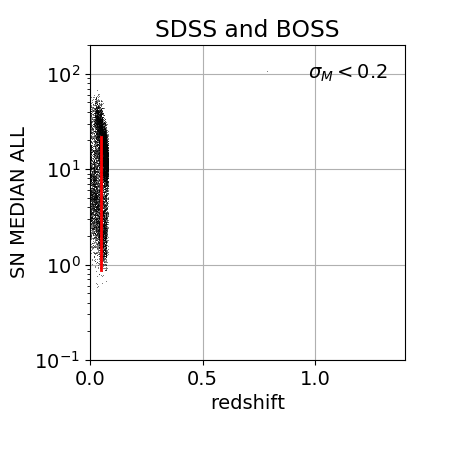
\includegraphics[height=4cm]{plots/SNR_ALL_redshift_sdss_boss.png}
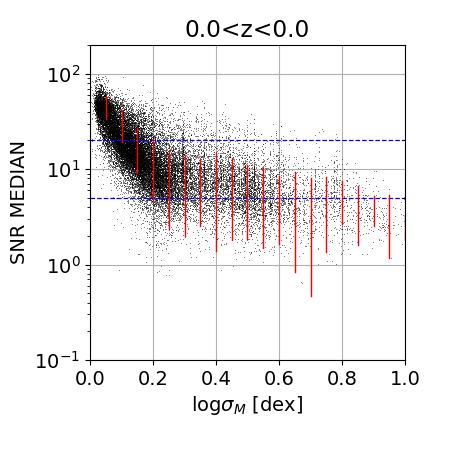
\includegraphics[height=4cm]{plots/SNR_39_41_stellar_mass_err_sdss_boss_00.png}
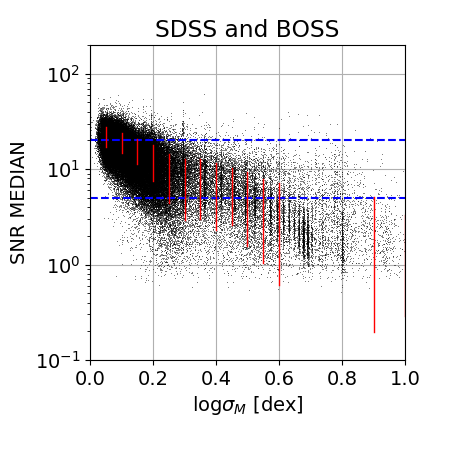
\includegraphics[height=4cm]{plots/SNR_41_55_stellar_mass_err_sdss_boss_02.png}
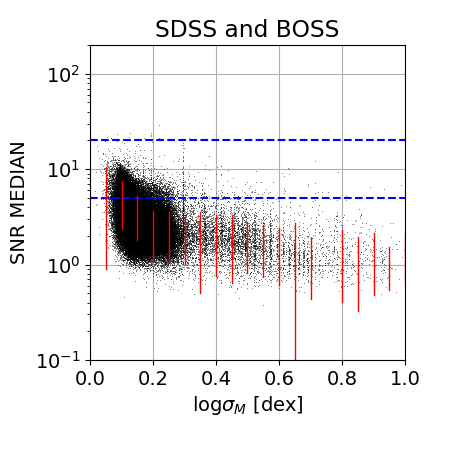
\includegraphics[height=4cm]{plots/SNR_55_68_stellar_mass_err_sdss_boss_04.png}
\end{center}
\end{figure*}



% \clearpage
%%%%%%%%%%%%%%%%%%%%%%%%%%%%%%%
%%%%%%%%%%%%%%%%%%%%%%%%%%%%%%%
% DATA
%%%%%%%%%%%%%%%%%%%%%%%%%%%%%%%
%%%%%%%%%%%%%%%%%%%%%%%%%%%%%%%
\section{Spectroscopic data}
\label{sec:DATA}

In this analysis, we consider galaxies from the SDSS and DEEP2 spectroscopic surveys. 
The redshift range spanned by the data is $0<z<1.7$ and most derived stellar masses are in the range $10^6 M_\odot$ to $10^{12.5} M_\odot$. 
The two surveys cover this parameter space in a complementary fashion. 
SDSS covers the most luminous galaxies over a wide area (order of 10,000 deg$^2$) and DEEP2 samples fainter galaxies (by about 2 magnitudes) over a small area (order of 2 deg$^2$). 
Fig. \ref{fig:nz} shows the redshift distribution of the two data sets. 
In both samples, the median signal to noise ratio per pixel in galaxy spectra with a robust redshift spans a wide range of values between 0.1 to 100, see Fig. \ref{fig:mass:redshift}. 
We comment on the correlation between signal to noise ratio and uncertainty on the stellar mass later in the paper. 
%
\subsection{SDSS}
We consider spectra obtained with the SDSS or BOSS spectrograph \citep{2006AJ....131.2332G,Smee2013} as in the fourteenth data release \citep{dawson_2016,blanton_2017,SDSS_DR14}. 
The SDSS (BOSS) spectrographs cover 3800-9200$\AA$ ($3650-10,400\AA$) at a resolution $1500$ at $3800\AA$ and $2500$ at $9000\AA$ with 3 (2) arc seconds diameter fibers.
Due to the variety of target selection algorithms successively applied to target galaxies within SDSS, the magnitude limit assumes different values. In the $i$-band, the different magnitude limits are mostly contained in the range 17 and 22.5. 

For the stellar population fitting, we consider objects classified as galaxies following criteria used in previous SDSS galaxy products\footnote{\url{http://www.sdss.org/dr12/spectro/galaxy/}}.
We consider objects for which a definite positive redshift was derived using galaxy templates 
(CLASS=="GALAXY", $Z>Z_{ERR}>0$, $ZWARNING==0$) in the current redshift pipeline \citep[][version v5\_10\_0]{2012AJ....144..144B}. 
For the data observed with the BOSS spectrograph, we consider the "NOQSO" version of these quantities. 
The obtain about 2.7 million optical galaxy spectra; $948,259$ million were observed with the SDSS spectrograph setup and with $1,759,362$ with the BOSS spectrograph setup, see Table \ref{table:single:spectra}. 


\begin{table*}
\caption{\label{table:single:spectra} Summary table of observed spectra and fit results. 
The Table is divided in four subsets, BOSS, SDSS, DEEP2 and DEEP2 \OII galaxies.
The last set shows the subset of the DEEP2 set that have a detection with a signal to noise ratio greater than 5 of the \OII emission line. 
The first line in each subset gives the total number of spectra available in the survey and how many of them are considered as galaxies. 
The assumed fitting setup (model and IMF)  is given in the first 2 columns. 
The third column gives the number of galaxies for which the fit converged. 
The last two columns gives the number of galaxies for which the stellar mass parameter is constrained within less than 0.4 dex and 0.2 dex, respectively. 
The number in parenthesis give the percentage relative to the total number of galaxies.}
%The obtain about 2.7 million optical galaxy spectra; $948,259$ million were observed with the SDSS spectrograph setup and with $1,759,362$ with the BOSS 
\begin{center}
\begin{tabular}{ll rrr}
\hline \hline
\multicolumn{5}{c}{eBOSS DR14: $1,759,362$ galaxies} \\
IMF &
Library & 
fit constrained & 
$\sigma_{\log_{10}M}<0.4$ dex & 
$\sigma_{\log_{10}M}<0.2$ dex \\ \hline
Chabrier & ELODIE & $1678846$ (95.4) & $1427861$ (81.2) & $980810$ (55.7) \\ 
Chabrier & MILES & $1632471$ (92.8) & $1529842$ (87.0) & $1237575$ (70.3) \\ 
Chabrier & STELIB & $1532700$ (87.1) & $1466376$ (83.3) & $1217235$ (69.2) \\ 
Kroupa & ELODIE & $1682734$ (95.6) & $1446616$ (82.2) & $1012728$ (57.6) \\ 
Kroupa & MILES & $1638112$ (93.1) & $1556522$ (88.5) & $1278732$ (72.7) \\ 
Kroupa & STELIB & $1539613$ (87.5) & $1490832$ (84.7) & $1252335$ (71.2) \\ 
Salpeter & ELODIE & $1681799$ (95.6) & $1467855$ (83.4) & $1047431$ (59.5) \\ 
Salpeter & MILES & $1647045$ (93.6) & $1583900$ (90.0) & $1351031$ (76.8) \\ 
Salpeter & STELIB & $1546335$ (87.9) & $1504425$ (85.5) & $1270344$ (72.2) \\ 
\hline 
 \multicolumn{5}{c}{SDSS DR14: $948,259$ galaxies} \\
IMF &
Library & 
fit constrained & 
$\sigma_{\log_{10}M}<0.4$ dex & 
$\sigma_{\log_{10}M}<0.2$ dex \\ \hline
Chabrier & ELODIE & $919507$ (97.0) & $886081$ (93.4) & $729736$ (77.0) \\ 
Chabrier & MILES & $919494$ (97.0) & $901024$ (95.0) & $765905$ (80.8) \\ 
Chabrier & STELIB & $894174$ (94.3) & $882412$ (93.1) & $722856$ (76.2) \\ 
Kroupa & ELODIE & $920373$ (97.1) & $892330$ (94.1) & $760271$ (80.2) \\ 
Kroupa & MILES & $919724$ (97.0) & $905489$ (95.5) & $798735$ (84.2) \\ 
Kroupa & STELIB & $897219$ (94.6) & $890963$ (94.0) & $752197$ (79.3) \\ 
Salpeter & ELODIE & $921261$ (97.2) & $896355$ (94.5) & $774556$ (81.7) \\ 
Salpeter & MILES & $920451$ (97.1) & $909374$ (95.9) & $814850$ (85.9) \\ 
Salpeter & STELIB & $898522$ (94.8) & $894546$ (94.3) & $768726$ (81.1) \\ 
\hline 
\multicolumn{5}{c}{DEEP2 DR4: $34,972$ galaxies $0.7<z<1.2$} \\
IMF &
Library & 
fit constrained & 
$\sigma_{\log_{10}M}<0.4$ dex & 
$\sigma_{\log_{10}M}<0.2$ dex \\ \hline
Chabrier & ELODIE& $20283$ (58.0) & $8656$ (24.8) & $3986$ (11.4) \\ 
Chabrier & MILES& $20214$ (57.8) & $10935$ (31.3) & $4619$ (13.2) \\ 
Chabrier & STELIB& $19807$ (56.6) & $11084$ (31.7) & $2733$ (7.8) \\ 
Kroupa & ELODIE& $20777$ (59.4) & $9524$ (27.2) & $4335$ (12.4) \\ 
Kroupa & MILES& $20544$ (58.7) & $11689$ (33.4) & $5238$ (15.0) \\ 
Kroupa & STELIB& $20272$ (58.0) & $12076$ (34.5) & $3350$ (9.6) \\ 
Salpeter & ELODIE& $20971$ (60.0) & $10042$ (28.7) & $4577$ (13.1) \\ 
Salpeter & MILES& $20760$ (59.4) & $12150$ (34.7) & $5541$ (15.8) \\ 
Salpeter & STELIB& $20417$ (58.4) & $12573$ (36.0) & $3708$ (10.6) \\ 
\hline 
\multicolumn{5}{c}{DEEP2 DR4: $19,656$ \OII galaxies $0.7<z<1.2$} \\
IMF &
Library & 
fit constrained & 
$\sigma_{\log_{10}M}<0.4$ dex & 
$\sigma_{\log_{10}M}<0.2$ dex \\ \hline
Chabrier & ELODIE & $10804$ (55.0) & $3829$ (19.5) & $1537$ (7.8) \\ 
Chabrier & MILES & $10192$ (51.9) & $5023$ (25.6) & $2080$ (10.6) \\ 
Chabrier & STELIB & $10356$ (52.7) & $4807$ (24.5) & $1149$ (5.8) \\ 
Kroupa & ELODIE & $11110$ (56.5) & $4317$ (22.0) & $1644$ (8.4) \\ 
Kroupa & MILES & $10332$ (52.6) & $5241$ (26.7) & $2267$ (11.5) \\ 
Kroupa & STELIB & $10641$ (54.1) & $5286$ (26.9) & $1344$ (6.8) \\ 
Salpeter & ELODIE & $11265$ (57.3) & $4613$ (23.5) & $1744$ (8.9) \\ 
Salpeter & MILES & $10550$ (53.7) & $5529$ (28.1) & $2425$ (12.3) \\ 
Salpeter & STELIB & $10735$ (54.6) & $5478$ (27.9) & $1478$ (7.5) \\ 

\hline
\end{tabular}
\end{center}
\end{table*}


For each SDSS (eBOSS) program, Tables 
\ref{ref:table:sdss:src:firefly}
(\ref{ref:table:boss:src:firefly}), 
\ref{ref:table:sdss:src:SNR} 
(\ref{ref:table:boss:src:SNR}), 
\ref{ref:table:sdss:src:fibermag} 
(\ref{ref:table:boss:src:fibermag}) 
describe the data set considered in its fullest. 

Table 
\ref{ref:table:sdss:src:firefly} (\ref{ref:table:boss:src:firefly})
gives the number of galaxies considered for the fit and the fraction where the stellar mass parameter was constrained. 
In SDSS, the target type 'GALAXY' has a constrained stellar mass for more than 95\% of its galaxy spectra where the median signal to noise ratio in the spectrum is positive. 
More than 80\% have an uncertainty on the stellar mass parameter lower than 0.2 dex. 
In eBOSS, the dominant galaxy type is LRG and 60\% have a stellar mass uncertainty lower than 0.2 dex. 
Table 
\ref{ref:table:sdss:src:SNR} (\ref{ref:table:boss:src:SNR}) 
gives for five redshift bins (with boundaries $0$, $0.025$, $0.375$, $0.7$, $0.85$, $1.6$) the fraction of galaxies that has a median SNR greater than 5 or 20. For redshifts $z<0.375$ more than half of the galaxies have a SNR greater than 20. For redshifts $z>0.7$ no galaxy has a SNR greater than 5. 
Table 
\ref{ref:table:sdss:src:fibermag} (\ref{ref:table:boss:src:fibermag}) 
gives, in three redshift bins (with boundaries $0$, $0.17$,  $0.55$, $1.6$), the fraction of galaxies where the fraction of the light in the fiber compared to the total light is greater than 50\% (10\%) i.e. the fiber magnitude smaller than the total magnitude by no more than 0.75 mag (2.5 mag). 
At redshift $z<0.17$, most SDSS galaxies have between 10 and 50\% of the light in the fiber, indeed their extension is larger than the fiber size.  
At high redshift $z>0.55$, more than a third of the eBOSS LRG galaxies have more than 50\% of their light reaching the fiber.


% and compares to previous SDSS galaxy products\footnote{\url{http://www.sdss.org/dr14/spectro/galaxy/}}. 
Compared to previous stellar population model catalogs, we roughly double the number of stellar masses measured \citep[DR12][]{Maraston2013,Thomas2013a}. % with an error smaller than $\pm0.2$dex . 
In particular the number of well-constrained stellar masses (i.e. constrained to better than 0.2 dex at given IMF) has also doubled. 
Such a gain in precision is enabled by fitting every pixel of the spectra rather than fitting the broad-band magnitudes (photometry) at the spectroscopic redshift. 
However, this is at the cost of having a less homogeneous sample. 
Indeed, the uncertainty on the stellar population parameters derived from full spectral fitting depends on the signal to noise ratio obtained in individual spectra, which varies according to observing conditions, position in the spectrograph and survey strategy. 
Hence, the tighter constrain on stellar parameters is gained at the price of completeness. 
The left panel on Fig. \ref{fig:mass:redshift} shows how the median signal to noise in good pixels are distributed with redshift. 
Low redshift galaxies ($z<0.4$) were observed on average at higher signal to noise ratio than higher redshift galaxies.
The other panels of Fig. \ref{fig:mass:redshift} show how the median signal to noise in good pixels in a band around the $4000\AA$ break correlates with the uncertainty on the stellar mass (for 3 redshift bins, $0<z<0.1$, $0.2<z<0.3$ and $0.4<z<0.5$).  
%The dependence of  
%We provide stellar population properties for three initial mass functions, and three libraries of templates; see next section about the details on the model.

The complete set of observed spectra we processed occupies about 0.8T of disk space.
The data considered for fitting in this analysis is available via the SDSS server,
\begin{itemize}
\item BOSS spectrograph data\\ \url{https://dr14.sdss.org/sas/dr14/eboss/spectro/redux/v5_10_0/spectra/PLATE/spec-PLATE-MJD-FIBERID.fits}. 
\item SDSS spectrograph data\\ \url{https://dr14.sdss.org/sas/dr14/sdss/spectro/redux/26/spectra/PLATE/spec-PLATE-MJD-FIBERID.fits}.
\end{itemize}
The data model for the spectra is described here \url{https://data.sdss.org/datamodel/files/BOSS_SPECTRO_REDUX/RUN2D/spectra/PLATE4/spec.html}. 

\subsection{DEEP2}
%For the VIPERS sample (REF), we consider the spectra that have a redshift $0.01<Z<1.4$. Out of the $91,507$ entries in the spectroscopic catalog, $87,762$ fulfill this condition. For VVDS Wide and Deep \citep{lefevre2013VVDS}, we apply the same condition and in the catalogs that contain $26,871$; $11,093$, respectively, we use $23,198$, $9,448$ spectra. 
DEEP2 is a deep pencil beam survey that acquired spectra for galaxies brighter than $R<24.1$ to study the evolution of galaxies. The survey is split in four fields that cover 2.7 deg$^2$  \citep{Newman_2013}. 
The DEIMOS spectrograph at Keck was used, which covers approximately the wavelength range $6500-9300\AA$ at a resolution $\sim$6000 \citep{Faber2003}. It accommodates order of 120 slits per mask. 
Although DEEP2 is a major galaxy evolution survey and stellar masses for galaxies observed by DEEP2 are mentioned in many publications, there does not seems to be a public stellar mass catalog available online for comparison \citep{kassin2007,covington2010,mostek2013,2017ApJ...838...87C}. 

In this analysis we consider the galaxy spectra that have a redshift in the range $0.001<z<1.7$ and that are classified with a flag $Z\_FLG\geq2$. 
Because the fitting requires the 4000$\AA$ break to be covered to recover the stellar age properly, we further constrain the redshift range to $0.7<z<1.2$. 
We use flux-calibrated spectra produced by \citet{Comparat2016LFs}. 
Out of the $50,319$ entries in the DEEP2 DR4 catalog, $34,972$ are considered for a stellar population model fit \textcolor{red}{and $XXXX$ with $0.7<z<1.2$}, see Table \ref{table:single:spectra} for the detailed numbers. 
To compare to the numbers obtained in \citet{Comparat2016LFs}, we further divided the data after the eventual detection of emission line in the spectrum. 

%One of the DEEP2 fields is located in the AEGIS\footnote{\url{http://aegis.ucolick.org}} field where deep multi-wavelength data is available.

The spectra used in this analysis were obtained via the DEEP2 server, here: \url{http://deep.ps.uci.edu/DR4/spectra.html}. 
The subset of processed flux-calibrated spectra are available here \url{https://firefly.mpe.mpg.de/v1_1_0/DEEP2/spectra}. Slits compared to fiber provide a larger fraction of the light emitted. \textcolor{red}{give actual numbers}

%%%%%%%%%%%%%%%%%%%%%%%%%%%%%%%
%%%%%%%%%%%%%%%%%%%%%%%%%%%%%%%%
% model
%%%%%%%%%%%%%%%%%%%%%%%%%%%%%%%
%%%%%%%%%%%%%%%%%%%%%%%%%%%%%%%%
\section{Stellar population modeling}
\label{sec:SPS}

We adopt the code \textsc{Firefly} \citep{firefly2017MNRAS} and the stellar population models of \citet{Maraston_2011} with different options for the Initial Mass Function (IMF) and input stellar library (see \ref{subsec:parameters}).

\subsection{Firefly fitting routine}
\textsc{Firefly}
\footnote{\url{http://www.icg.port.ac.uk/firefly}} 
is a chi-squared minimization fitting code that for a given input observed Spectral Energy Distribution (SED), 
compares combinations of single-burst stellar population models (SSP), 
following an iterative best-fitting process controlled by the Bayesian 
Information Criterion (BIC) until convergence is achieved. 
An important feature of our code is that no priors - other than the assumed models - are applied, rather all solutions within a statistical cut are retained with their weight.
The weight of each component can be arbitrary and no regularization or additional prior than the adopted model grid is applied. 
We account for dust attenuation in a novel way, fully described in \citet{firefly2017MNRAS} which we summarise here. 
We deduce the attenuation affecting an observed spectrum by the distortion of the continuum. 
%of the observed spectra with respect to the model spectra with the same parameters. 
%For obtaining the actual parameters of the observed spectrum, 
We rectify the continuum shape %(in other words we 'rectify' the spectra) 
of both observations and models by multiplying them by a function, referred to as High-Pass Filter, (HPF). 
It removes the large-scale modes of the spectra occurring on widths larger than $\sim~100$\AA. 
We find the best-fitting stellar population model between HPF rectified data and models. 
It consists essentially in matching the absorption features. 
After a best fitting model is found, we compare it to the original (not rectified) observed spectrum. The difference between the two is used to obtain an attenuation array (i.e. flux ratios per wavelength). 
The returned attenuation array is then matched to known analytical approximations to return an E(B-V) value. 
This procedure allows for removal of large scale modes of the spectrum associated with dust and/or poor flux calibration.	
\textsc{Firefly} provides light- and mass-weighted stellar population properties (age and metallicity), E(B-V) values and stellar mass for the most likely best fitting model and all of its SSP components.  
Errors on these properties are obtained by the likelihood of solutions within the statistical cut. 

The fitting routine follows these steps.
\begin{enumerate}
\item Match the resolution of the models to that of the data (usually, downgrading the models)
\item Mask emission lines.
\item Determine dust attenuation in the continuum.
\item Get the best fitting stellar population model as a linear combination of single-burst models.
\item Compute the light- and mass-weighted synthetic stellar population contributions.
\item Convert $\chi^2$ into probabilities and calculates average properties and errors (both mass weighted and light weighted).% (It assumes that the number of degrees of freedom is the number of wavelength points);
%\item Subtract the model of the continuum from the composite to obtain the emission-line composite.
%\item Fit emission line fluxes as in C16 for both the composite and the emission-line composite.
\end{enumerate}
For full details about the \textsc{Firefly} code please turn to \citet{firefly2017MNRAS}. 
The code and the models used to create this dataset are public via the SDSS server:
\begin{itemize}
\item Fitting code. The official website of the \textsc{Firefly} team is \url{http://www.icg.port.ac.uk/firefly} links to the official maintained version of the \textsc{firefly} software. 
\item Stellar population models: \url{https://svn.sdss.org/public/data/sdss/stellarpopmodels/tags/v1_0_2/} 
%\item A development version of the code where you may find scripts for running fits on large computer infrastructure is available here \url{https://github.com/JohanComparat/firefly_code} (this is only informative)
\end{itemize}
%Note that the official version is ahead (v1\_1) of the version It is important to note the following. 
%As `stellar mass' in the SDSS data release (v1\_0\_4 run finalized mid 2017), we only output the total mass that went into stars. 
%In the most recent version (v1\_1\_0, run finalized end 2017), instead, 
We output the actual (present) stellar mass, including its fraction locked in stellar remnants (white dwarfs, neutron stars and black holes) or lost via stellar evolution (returned fraction). 
%The extended v1\_1 level catalogs are available at the MPE mirror. 
%They will be available through the SDSS mirror for the next data release DR16, see Sec. \ref{subsec:alt:cat}

\subsubsection{Effect of wavelength}
\citet{firefly2017MNRAS} showed (section 5.2, Fig. 19) that to reliably recover of the age, the 4000$\AA$ break region is needed in the observations. This is not a problem for the SDSS+eBOSS observations. This is an issue for the DEEP2 spectra that only cover the wavelength range 6500 − 9300$\AA$ i.e. accurate ages for the DEEP2 galaxies can be recovered only if the redshift is in the window 3800(1+z)$>$6500 and 4200(1+z)$<$9300 i.e. $0.7<z<1.2$.

\subsubsection{Comparison with previous measurements}
\citet{firefly2017MNRAS} compared (section 6.2, Figs. 24, 25) the \textsc{firefly}-SDSS measurements to the results from \textcolor{red}{Cid-Fernandes et al. (2005) and from Tojeiro et al. (2009)}. In both cases, a good wualitative agreement was found.

\subsection{Performances}
\label{subsec:firefly:performances}
The code is able to recover stellar population properties such as age, metallicity, and stellar mass, and the star formation history, 
down to an SNR$\sim5$, for moderately dusty systems (E(B-V)<0.75). 
At SNR$\sim20$, the recovery of the star formation history is remarkably good independently of reddening, unless the star formation is very extended ($\sim$10 Gyr). 
At lower SNR down to SNR$\sim0.5$, we find that the stellar masses are in agreement (within errors) with previous estimates based on SED fitting on broad band magnitudes. 
At such low SNR, the full star formation history cannot be reconstructed accurately. The age-metallicity degeneracy also becomes important and the individual stellar ages and stellar metallicities are uncertain.

The median SNR in all good pixels in the $i$-band of the spectrum is anticorrelated to the uncertainty on the stellar mass. The higher the SNR, the smaller the uncertainty on the stellar mass, see Fig. \ref{fig:mass:redshift}.\footnote{Chen et al. 2012 achieved a similar conclusion by comparing the stellar mass obtained via their PCA-based full spectral fitting and the one from broad-band SED fitting. The two estimates converge at a $SNR$~around 25. See also discussion in Maraston et al. 2013, Appendix.} 
This correlation holds up to redshift 0.4-0.5. 
Then the band of importance between $3500$-$5500\AA$ break starts to enter the $z$-band where the estimation of the SNR are much noisier. 
So, at lower redshift, selecting the best fits can be done by either a selection on the SNR or on the uncertainty on the stellar mass. 
At higher redshift, the median SNR measure provided in the SDSS specObj summary files is not a reliable estimate of the actual SNR. 
%To have a better handle, we would need to estimate median SNR in the $i$ or $z$-band with a mask for the sky OH lines applied. 

We follow the \citet{2013AJ....145...69L} procedure to mask pixels affected by the sky and estimate SNR in a cleaner fashion, we call it the effective signal to noise ratio SNR$_{eff}$. 
Due to time constraints, we only perform this study on a subset of the complete sample. 
We find that in the high SNR regime ($SNR>10$), estimations are converging. 
In the range 1-10, we find large disagreement between the two SNR estimators. 
For a part of the galaxy population observed, the SN\_MEDIAN\_ALL estimator underestimates the SNR by a factor 3 to 5 compared to SNR$_{eff}$. 
The galaxies with an underestimated SNR (1 instead of 5) have tightly constrained firefly parameters. 
So that using this SNR$_{eff}$, the correlation with uncertainty on the stellar mass holds down to low SNR$_{eff}$ and to high redshift. 
We introduce two thresholds of 0.2 and 0.4 dex uncertainty on the stellar mass that relate to SNR$_{eff}$ around 20 and 5 where performances were previously quantified. The newly estimated effective SNR are available in the summary tables.

To construct a sample based on the summary files, we advise the user to pre-select the sample of interest in SNR. Tables in appendix give the breakdown as a function of target types of the fraction of targets with a SNR greater than 5 and 20. Note that studies needing high SNR$>20$ will be intrinsically limited to low redshift.
%We therefore rely on the estimated uncertainty on the stellar mass to select the best sample at each redshift. At low redshift, this is equivalent to using the available SNR estimate. 
%For the next release, we will add the estimates of SNR$_{eff}$ for all spectra to track optimally the code's performances. 

%In all catalogs provided, the median signal to noise ratio in good pixel of each spectrum is given so that the user may select according to the precision he wishes.
\subsection{\citet{Maraston_2011} models}

We use the \citet{Maraston_2011} stellar population models. 
They assume different input stellar libraries, of which we use three, namely :
\begin{itemize}
\item STELIB, covering 3200–9300$\AA$ with a 3.4$\AA$ sampling at 5500$\AA$ i.e. at a resolution $R=1617$ \citep{leborgne2003},  
\item MILES, covering 3500–7430$\AA$ with a 2.54$\AA$ sampling at 5500$\AA$ i.e. at a resolution $R=2165$ \citep{MILES_2006,MILES_2011},
\item ELODIE, covering 3900–6800$\AA$ with a 0.55$\AA$ sampling at 5500$\AA$ i.e. at a resolution $R=10000$ \citep{Prugniel2007}.
\end{itemize}
Recall that SDSS, BOSS and DEIMOS cover 3800-9200, 3650-10,400, 6500-9300 at R$\sim$2000, 2000, 6000. The mismatch between the wavelength coverage of DEEP2 and those models explain the lack of fits at low redshift. It is part of an ongoing effort to complete the low-redshift extension of DEEP2 with IR extended models, which we shall release in the future.
Figure \ref{fig:distributions:10Gyr:models} shows a model of a 10 Gyr old stellar population with solar metallicity for the three libraries and three IMFs. It illustrates that the change in library corresponds mainly to a change of resolution and wavelength coverage and that the change in IMF corresponds to a change in the normalization of the flux emitted.

\begin{figure}
\begin{center}
\caption{\label{fig:distributions:10Gyr:models} 
Model of a 10 Gyr old stellar population with solar metallicity with a flux normalized to 1 solar mass. The top, middle, bottom plots show the model based on STELIB, MILES and ELODIE libraries. 
The left column shows the whole models and the right column the zoom on the 4000$\AA$ break region (3900$\AA$-4400$\AA$), most important for age determination. 
For each model are shown the corresponding curves for each IMF, that induce only a change in the flux normalization. 
The STELIB model has the largest wavelength coverage with the lowest resolution, then the MILES (medium resolution) and then the ELODIE (highest resolution).
In the zoomed in plots, we see that the main Calcium absorption lines are present in the three resolutions, but you can note some substructure between the Ca H and the Ca K absorption is clearly visible in the highest resolution ELODIE templates, less visible in the MILES and absent from the STELIB. 
It stresses the importance of resolution matching before fitting.
}  
%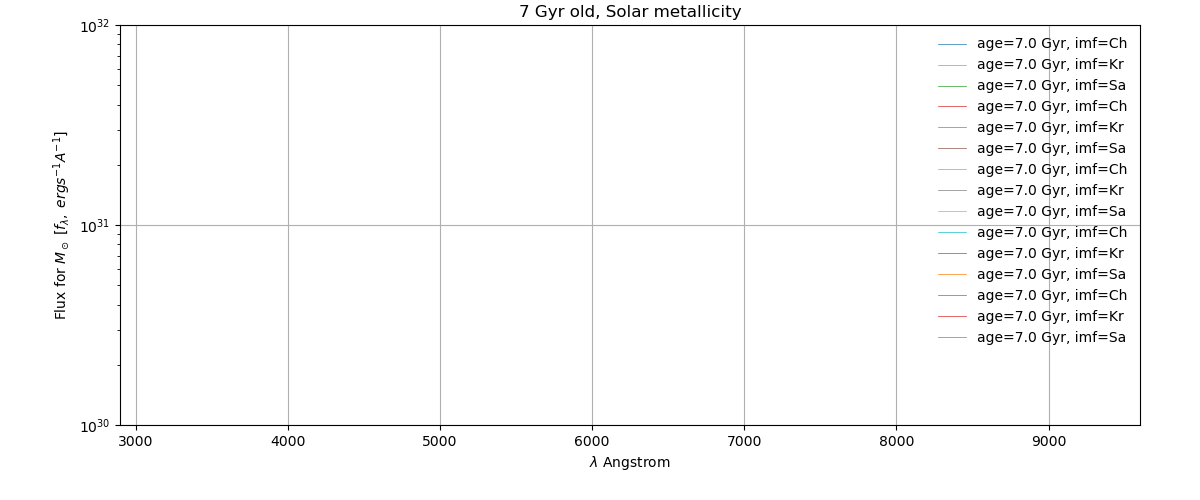
\includegraphics[height=8cm]{/home/comparat/software/firefly_explore/data/images/models/Zsun_7Gyr_all_models.png}
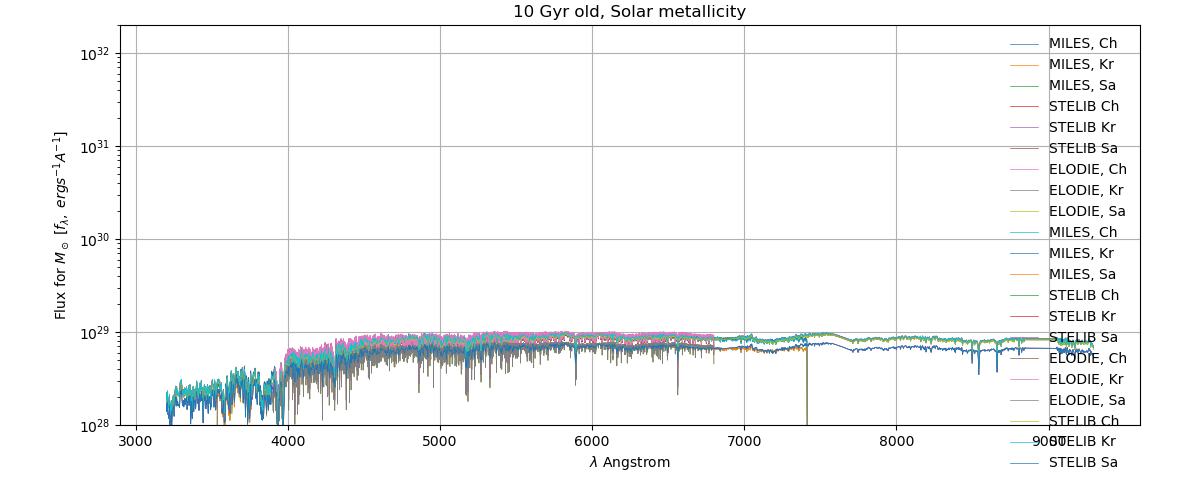
\includegraphics[width=8cm]{/home/comparat/software/firefly_explore/data/images/models/Zsun_10Gyr_STELIB_models.png}
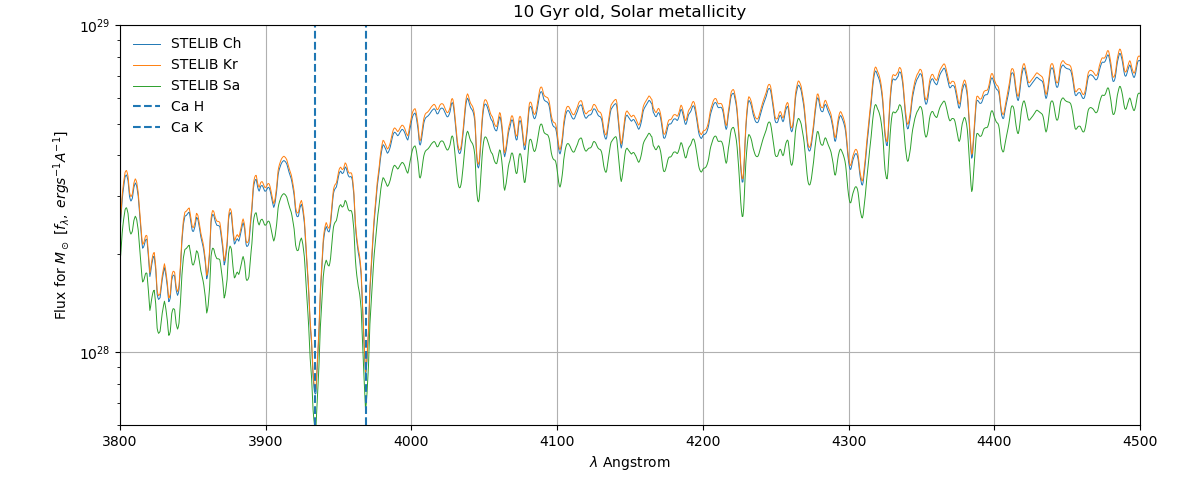
\includegraphics[width=8cm]{/home/comparat/software/firefly_explore/data/images/models/Zsun_10Gyr_STELIB_models_38_45.png} \\

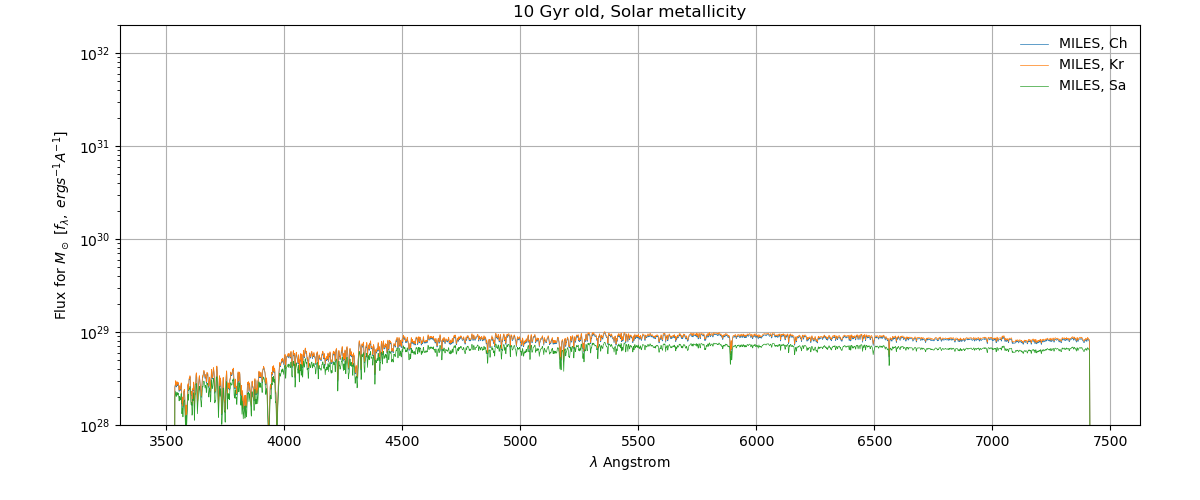
\includegraphics[width=8cm]{/home/comparat/software/firefly_explore/data/images/models/Zsun_10Gyr_MILES_models.png}
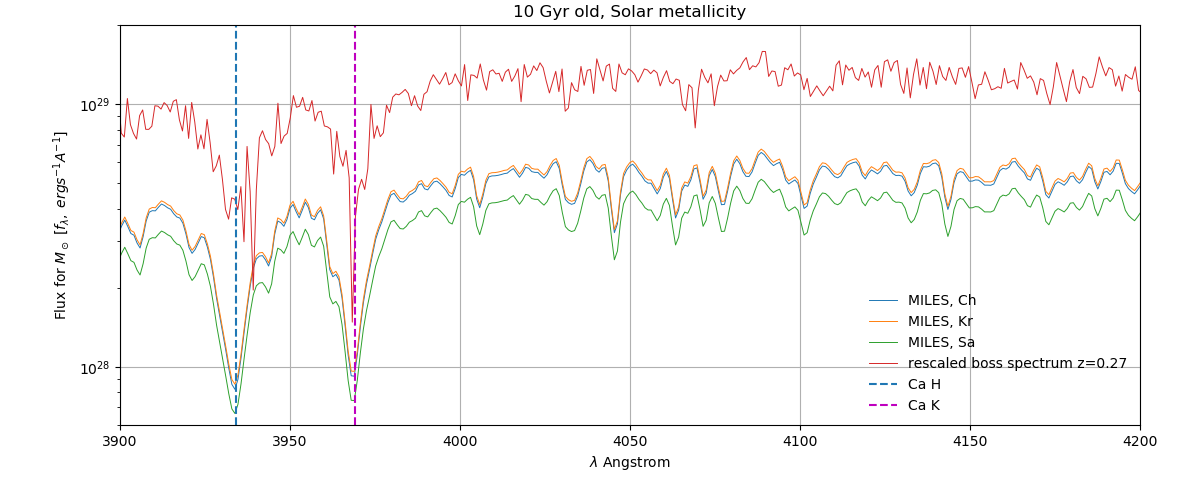
\includegraphics[width=8cm]{/home/comparat/software/firefly_explore/data/images/models/Zsun_10Gyr_MILES_models_38_45.png} \\

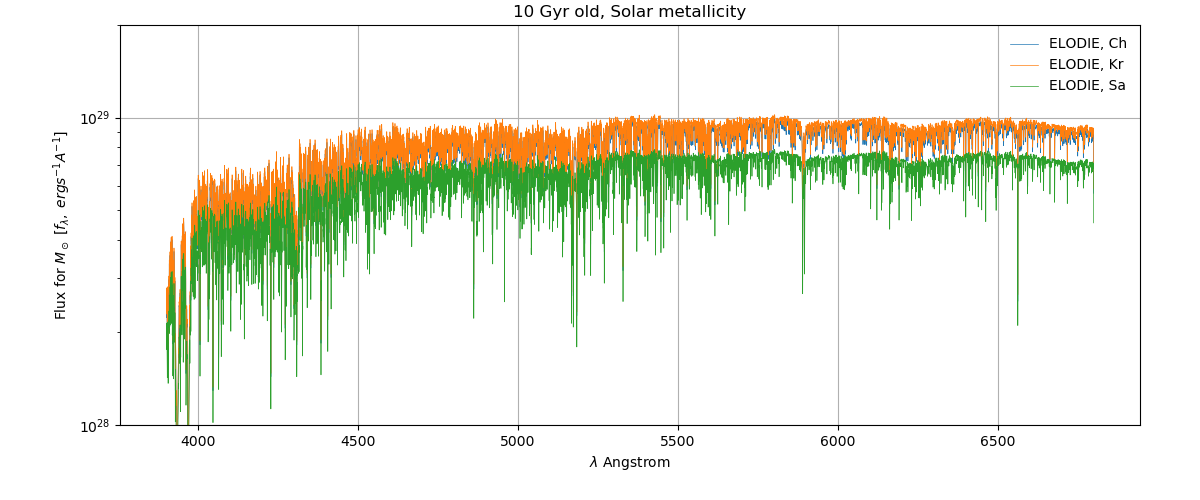
\includegraphics[width=8cm]{/home/comparat/software/firefly_explore/data/images/models/Zsun_10Gyr_ELODIE_models.png}
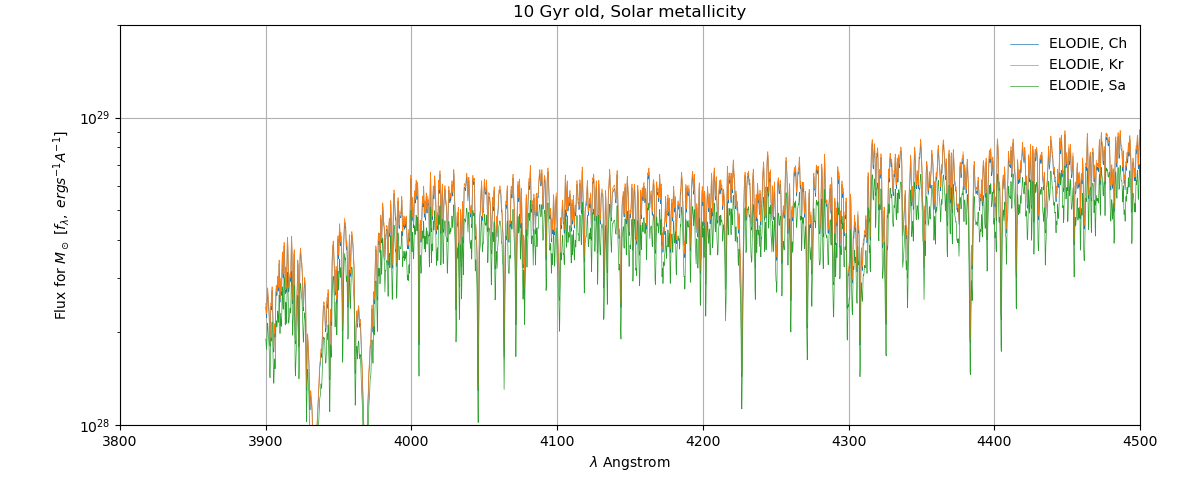
\includegraphics[width=8cm]{/home/comparat/software/firefly_explore/data/images/models/Zsun_10Gyr_ELODIE_models_38_45.png}
\end{center}
\end{figure}

% 
% \begin{figure}
% \begin{center}
% \caption{\label{fig:distributions:10Gyr:models:zoom} 
% Same as Fig. \ref{fig:distributions:10Gyr:models} zoomed in on the 4000$\AA$ break region (3900$\AA$-4400$\AA$). 
% The difference in resolution is seen in the number of spectral features existing in the models. 
% The main Calcium absorption lines are present in the three resolutions, but you can note some substructure between the Ca H and the Ca K absorption is clearly visible in the highest resolution ELODIE templates, less visible in the MILES and absent from the STELIB. 
% %This motivates the need of downsampling the models to the resolution of the data.
% }  
% %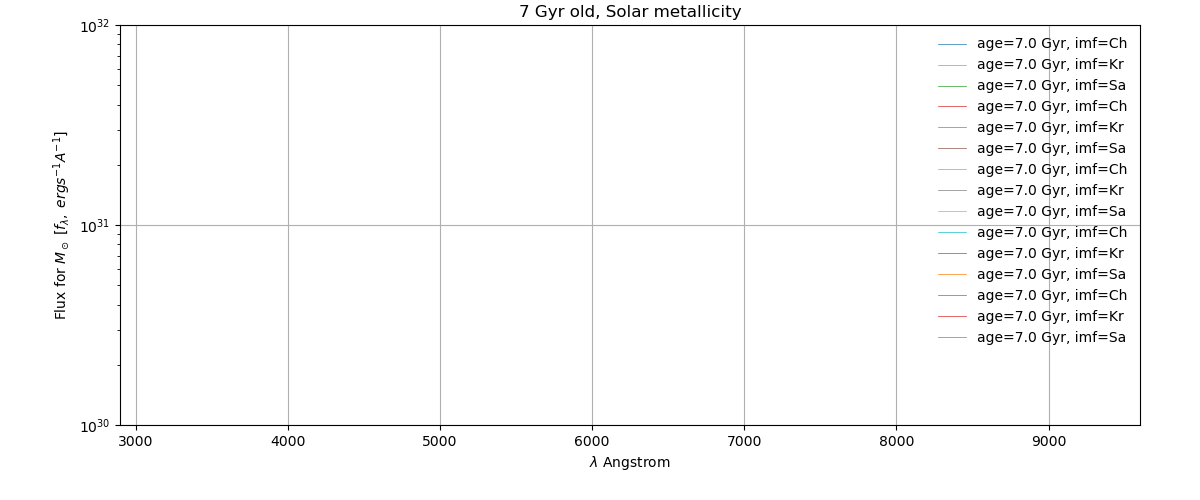
\includegraphics[height=8cm]{/home/comparat/software/firefly_explore/data/images/models/Zsun_7Gyr_all_models.png}
% \end{center}
% \end{figure}

\subsection{Parameters of the run}
\label{subsec:parameters}

For this run, we repeat the computation for the following three choices of the stellar initial mass function (IMF):
\begin{itemize}
\item Salpeter, \citet{Salpeter_1955},  
\item Chabrier, \citet{Chabrier2003}, 
\item Kroupa, \citet{Kroupa2001}. 
\end{itemize}
and for each of the input M11 models described above (namely, M11-ELODIE, M11-MILES and M11-STELIB).
The toal number of parameters used in the models are M11-STELIB: 85, M11-ELODIE: 132, M11-MILES: 156. 
In total, we provide up to nine models (depending on whether 
the parametter 'stellar mass' results to be constrained) of the continuum for each galaxy considered. 

The grid of models spans ages in the range $10^{6}<Age [yr]< 2 \times 10^{10}$ and metallicities in the range $-3<\log_{10}(Z/Z_\odot)<3$, with each M11 model spanning a different age/metallicity grid \citep[cfr.][Table1]{firefly2017MNRAS}. 
The E(B-V) parameter is constrained to the range 0-0.7. 
The main degeneracies are between age and metallicity and between E(B-V) and stellar mass.
% (age less than 10 for v1\_0\_4)

Differences corresponding to the various initial parameter choices are discussed later in the paper.

\subsection{Processing}
The processing was done on  SCIAMA\footnote{\url{http://www.sciama.icg.port.ac.uk/}}, a high performance computing facility belonging to the University of Portsmouth (United Kingdom). 
A fit for a single model takes about a minute cpu so that the whole run required about 350,000 cpu hours. 
The total data volume is about 3.2T, as in Table \ref{table:processing}.
\begin{table}
\caption{\label{table:processing} Data volume generated in this study.}
\begin{center}
\begin{tabular}{ccccc}
\hline \hline
Survey &
catalog &
spectra & 
models & total \\ \hline
SDSS
& 23G
& 278G
& 860G 
& 1.1T \\
eBOSS
& 49G
& 0.5T 
& 1.5T 
& 2.1T \\
DEEP2 
& 1.4G
& 6.2G
& 17G
& 24.6G \\
\hline 
\end{tabular}
\end{center}
\end{table}

\subsection{Data}

For SDSS, all products are available here 
\url{https://firefly.mpe.mpg.de/v1_1_0/26}. 
For eBOSS, all products are available here 
\url{https://firefly.mpe.mpg.de/v1_1_0/v5_10_0}. 
A previous version of the SDSS/eBOSS firefly catalogs is available here 
\url{https://data.sdss.org/sas/dr14/eboss/spectro/firefly/v1_0_4}.
For DEEP2, they are available here 
\url{https://firefly.mpe.mpg.de/v1_1_0/DEEP2} (both versions).
For a visual explanation of the data model (three layers), please visit \url{http://www.sdss.org/dr14/spectro/eboss-firefly-value-added-catalog/}.

\subsubsection{Model spectrum}
The lowest level data product is the model file. 
There is one such file per galaxy spectrum considered. 
It is available for both DEEP2 and SDSS data sets. 
It is a fits file with a header and 9 data units. 
The primary header contains all input parameters used during the fit.
The following nine data units each contain 
\begin{itemize}
\item Header. The best fit parameters for each SSP entering the best model. 
\item Data extension. The best-fitting model spectrum: wavelength (Unit Angstrom) and model flux ($f_\lambda$ convention, unit $10^{-17}$ erg cm$^{-2}$ s$^{-1}$ A$^{-1}$). 
\end{itemize} 

The nine data units contain the results obtained for the different combinations of stellar libraries and initial mass functions. 
\begin{itemize}
\item HDU1 M11-MILES x Chabrier IMF
\item HDU2 M11-MILES x Salpeter IMF
\item HDU3 M11-MILES x Kroupa IMF
\item HDU4 M11-ELODIE x Chabrier IMF
\item HDU5 M11-ELODIE x Salpeter IMF
\item HDU6 M11-ELODIE x Kroupa IMF
\item HDU7 M11-STELIB x Chabrier IMF
\item HDU8 M11-STELIB x Salpeter IMF
\item HDU9 M11-STELIB x Kroupa IMF
\end{itemize}

The data model for this product, named 'spFly', is available here \url{https://data.sdss.org/datamodel/files/EBOSS_FIREFLY/FIREFLY_VER/RUN2D/SPMODELS_VER/PLATE/spFly.html} and the corresponding files here \url{https://firefly.mpe.mpg.de/v1_1_0/26/stellarpop} and here \url{https://firefly.mpe.mpg.de/v1_1_0/v5_10_0/stellarpop}. 
The DEEP2 result model spectra are provided here \url{http://www.mpe.mpg.de/~comparat/DEEP2/stellarpop/} and follow the naming convention 'spFly-deep2-MASK-OBJNUM.fits'.% 'spec/deep2-MASK-OBJNUM.fits' and their model

An automated summary plot is provided for each model file. 
It illustrates the spectrum, the models, and the fitted parameters, see Fig. \ref{fig:firefly:output}. 
It shows an example of these Figures for a galaxy at redshift $z=0.127$ identified by PLATE=0266, MJD=51602, FIBERID=0004. 
The top panel shows the observed spectrum (grey line) and the models (colored lines). 
The middle panel shows the normed distribution of the quantity (data-model)/error for each pixel considered in the fit and for each of the nine models. 
It is compared to a normal distribution that it should follow, if the fits are reliable (dashed black line named 'N(0,1)' in the legend). 
The bottom panel shows the output parameters stellar mass vs. stellar age for each of the nine models. 
Ages and masses are in good agreement. %The stellar metallicity differ slightly when changing given in the 
Such a Figure is created for each fitted spectrum and provided together with the models.


\begin{figure*}
\begin{center}
\caption{\label{fig:firefly:output}
Example of a fit taken from the first plate of SDSS considered in this analysis: 0266. 
The top panel shows the observed spectrum (grey line) and its models (colored lines). 
The middle panel shows the $\chi^2$ distribution per pixel for each fit compared to a normal distribution (labeled N(0,1), dashed line). 
The bottom panel shows the output parameters stellar mass (y-axis) vs stellar age (x-axis), which nicely agree. Each blue point refers to one of the nine models. The blue points are related to their respective caption by black arrows. 
This Figure is generated for each fit and is available in the data repository.}
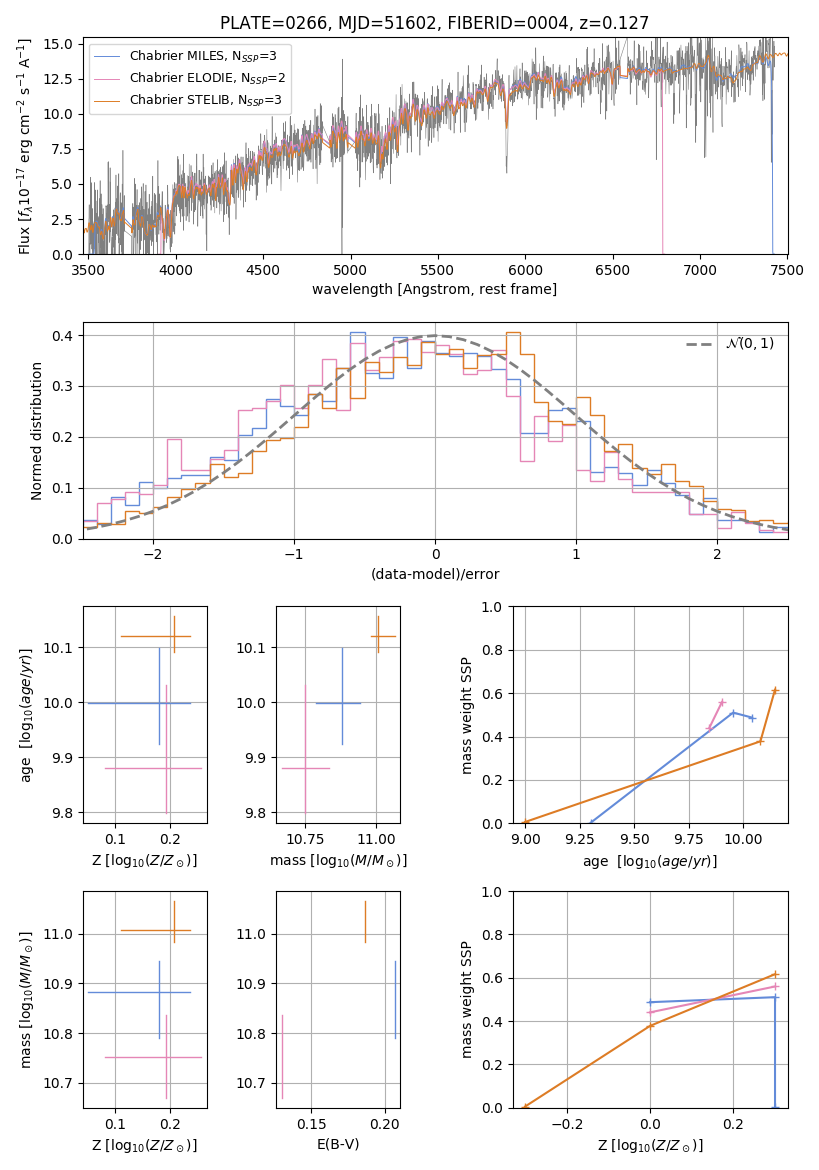
\includegraphics[width=14cm]{plots/spFly-0266-51602-0004.png}
\end{center}
\end{figure*}


\subsubsection{Plate-level summary catalogs (SDSS only)}
Due to the size of the SDSS data set and its structure, we create summary catalogs for each plate, named 'spFlyPlate'.
They contain all output parameters from the fitting procedure. 
The data model for these catalogs is given here 
\url{https://data.sdss.org/datamodel/files/EBOSS_FIREFLY/FIREFLY_VER/RUN2D/SPMODELS_VER/PLATE/spFlyPlate.html}. %This page gives the link to the plate catalogs.

For each spFlyPlate file, a representation of the data obtained is proposed, an example is displayed in 
Fig. \ref{fig:firefly:output:plate}. 
It shows the distribution of stellar age and stellar masses measured in plate (0266). It also shows a comparison of the stellar masses derived using the M11 models with the ELODIE stellar library and varying the IMFs. You may note the systematic offset in stellar masses when assuming a Salpeter or a Chabrier IMF (bottom left panel). 

As the DEEP2 data is much smaller than the SDSS, we did not create this second layer of summary files for DEEP2. 
% 
% \begin{figure*}
% \begin{center}
% \caption{\label{fig:firefly:output:plate}
% Summary plot for SDSS plate 0266. 
% It shows the cumulative normed distributions of stellar ages and stellar masses derived for all IMF + library setups (top row).
% The bottom panels compare the stellar masses derived assuming different IMFs. 
% It shows the known fact that the assumption of a Salpeter IMF implies stellar masses that are on average 30\% larger than those for Kroupa and Chabrier IMFs (bottom left panel).
% Chabrier and Kroupa IMFs give on average the same stellar masses (bottom right panel).}
% \includegraphics[width=14cm]{plots/spFlyPlate-0266-51602.png}
% %\includegraphics[width=14cm]{plots/spFly-0266-51602-0159.png}
% \end{center}
% \end{figure*}

\subsubsection{Summary catalogs}
Top-level summary catalogs contain all of the fitted parameters. They are available here 
\begin{itemize}
\item SDSS: \url{https://firefly.mpe.mpg.de/v1_1_0/26/sdss_firefly-26.fits}
\item eBOSS: \url{https://firefly.mpe.mpg.de/v1_1_0/v5_10_0/eboss_firefly-v5_10_0.fits}
\item DEEP2: \url{https://firefly.mpe.mpg.de/v1_1_0/DEEP2/catalogs/zcat.deep2.dr4.v4.LFcatalogTC.Planck13.spm.v2.fits.gz}
\end{itemize}
They can be download as follows
\begin{verbatim}
wget --no-check-certificate https://firefly.mpe.mpg.de/v1_1_0/26/sdss_firefly-26.fits .
\end{verbatim}

%In the SDSS case, the catalogs become too large when all parameters are written, so we created catalogs with only subsets of parameters. 
%In the case of DEEP2, the catalog is small enough that adding all parameters is still manageable. 
The data model for the summary file for the eBOSS data is available at: 
\url{https://data.sdss.org/datamodel/files/EBOSS_FIREFLY/FIREFLY_VER/RUN2D/eboss_firefly.html} while the one for the SDSS data \url{https://data.sdss.org/datamodel/files/EBOSS_FIREFLY/FIREFLY_VER/RUN2D/sdss_firefly.html}.
They differ by the redshift column: 'Z' for SDSS and 'Z\_NOQSO' for eBOSS.  
%These summary catalogs are also available in the SCI-SERVER CAS database\footnote{\url{http://www.sciserver.org/}}. 

%The DEEP2 summary file is available here and follows the same data model.
Assumptions in the IMF or templates induce systematic differences in the constrained parameters. 
Therefore, we do not provide a mean stellar mass based on these nine runs.

% \subsection{Additional catalogs}
% \label{subsec:alt:cat}
% Beyond the run described above, we did a number of other runs with different setups. 
% From these emerged valuable catalogs. 
% They are hosted here \url{www.mpe.mpg.de/~comparat/DEEP2/} or \url{www.mpe.mpg.de/~comparat/firefly_catalogs/} in the directory '\url{additional_catalogs}'. 
% Each catalog comes with a short 'readme' file that documents its purpose. 
% For example, we provide nine catalogs (one per IMF x library) with all the measured parameters of the star formation history. We also provide preliminary catalogs of the v1\_1 (accounting for remnants) that have slightly different metallicity and age boundary parameters.

\textbf{ADD DATA MODEL FOR THE SUMMARY FILES. Clarify all definitions with links to equations in the firefly paper.}

% SPECOBJID	str		Spectroscopic unique identifier
% OBJID	int		Photometric unique identifier
% RUN2D	str		version of the 2d reduction pipeline
% RUN1D	str		version of the 1d reduction pipeline
% MJD	int		MJD of observation
% PLATE	int		Plate number
% FIBERID	int		Fiber identification number
% PLUG_RA	Double		Right ascension of fiber, J2000
% PLUG_DEC	Double		Declination of fiber, J2000
% Z	float		Best redshift
% Z_ERR	float		Error in redshift
% ZWARNING	int		Warnings in "z" redshift
% CLASS	str		Classification in redshift
% SUBCLASS	str		Sub-classification in redshift
% Kroupa_age_lightW	float		light weighted age upper error, Kroupa IMF
% Kroupa_age_lightW_err_plus	float		light weighted age lower error, Kroupa IMF
% Kroupa_age_lightW_err_minus	float		light weighted stellar metallicity, Kroupa IMF
% Kroupa_metallicity_lightW	float		light weighted stellar metallicity upper error, Kroupa IMF
% Kroupa_metallicity_lightW_err_plus	float		light weighted stellar metallicity upper error, Kroupa IMF
% Kroupa_metallicity_lightW_err_minus	float		light weighted stellar metallicity lower error, Kroupa IMF
% Kroupa_stellar_mass	float		stellar mass, Kroupa IMF
% Kroupa_stellar_mass_err_plus	float		stellar mass upper error, Kroupa IMF
% Kroupa_stellar_mass_err_minus	float		stellar mass lower error, Kroupa IMF
% Kroupa_spm_EBV	float		reddenning fitted, Kroupa IMF
% Kroupa_nComponentsSSP	float		number of single stellar population components, Kroupa IMF
% Kroupa_chi2	float		chi squared, Kroupa IMF
% Kroupa_ndof	float		number of degrees of freedom, Kroupa IMF
% Salpeter_age_lightW	float		light weighted age upper error, Salpeter IMF
% Salpeter_age_lightW_err_plus	float		light weighted age lower error, Salpeter IMF
% Salpeter_age_lightW_err_minus	float		light weighted stellar metallicity, Salpeter IMF
% Salpeter_metallicity_lightW	float		light weighted stellar metallicity upper error, Salpeter IMF
% Salpeter_metallicity_lightW_err_plus	float		light weighted stellar metallicity upper error, Salpeter IMF
% Salpeter_metallicity_lightW_err_minus	float		light weighted stellar metallicity lower error, Salpeter IMF
% Salpeter_stellar_mass	float		stellar mass, Salpeter IMF
% Salpeter_stellar_mass_err_plus	float		stellar mass upper error, Salpeter IMF
% Salpeter_stellar_mass_err_minus	float		stellar mass lower error, Salpeter IMF
% Salpeter_spm_EBV	float		reddenning fitted, Salpeter IMF
% Salpeter_nComponentsSSP	float		number of single stellar population components, Salpeter IMF
% Salpeter_chi2	float		chi squared, Salpeter IMF
% Salpeter_ndof	float		number of degrees of freedom, Salpeter IMF
% Chabrier_age_lightW	float		light weighted age upper error, Chabrier IMF
% Chabrier_age_lightW_err_plus	float		light weighted age lower error, Chabrier IMF
% Chabrier_age_lightW_err_minus	float		light weighted stellar metallicity, Chabrier IMF
% Chabrier_metallicity_lightW	float		light weighted stellar metallicity upper error, Chabrier IMF
% Chabrier_metallicity_lightW_err_plus	float		light weighted stellar metallicity upper error, Chabrier IMF
% Chabrier_metallicity_lightW_err_minus	float		light weighted stellar metallicity lower error, Chabrier IMF
% Chabrier_stellar_mass	float		stellar mass, Chabrier IMF
% Chabrier_stellar_mass_err_plus	float		stellar mass upper error, Chabrier IMF
% Chabrier_stellar_mass_err_minus	float		stellar mass lower error, Chabrier IMF
% Chabrier_spm_EBV	float		reddenning fitted, Chabrier IMF
% Chabrier_nComponentsSSP	float		number of single stellar population components, Chabrier IMF
% Chabrier_chi2	float		chi squared, Chabrier IMF
% Chabrier_ndof	float		number of degrees of freedom, Chabrier IMF


\subsection{Description of the parameters obtained}
In this section, we present statistics of the four main parameters derived: dust, stellar age, stellar metallicity and stellar mass.

\subsubsection{Dust}
The dust is fitted first on the data and then assumed when fitting for the combination of SSPs. 
The library assumed makes quite a difference in the retrieved E(B-V). 
Fits done with STELIB (largest wavelength coverage) provide on average on lower values than MILES than ELODIE (smallest wavelength covrerage), see the distributions of the E(B-V) obtained in Fig. \ref{fig:distributions:EBV}. 

The IMF assumed doe not change the E(B-V) value fitted, as expected.

\begin{figure}
\begin{center}
\caption{\label{fig:distributions:EBV} 
Normed cumulative distribution of the E(B-V) fitted. The IMF assumed does not make a difference. Due to different wavelenght coverage the library assumed, the E(B-V) values measured differ by up to 0.2 dex.}  
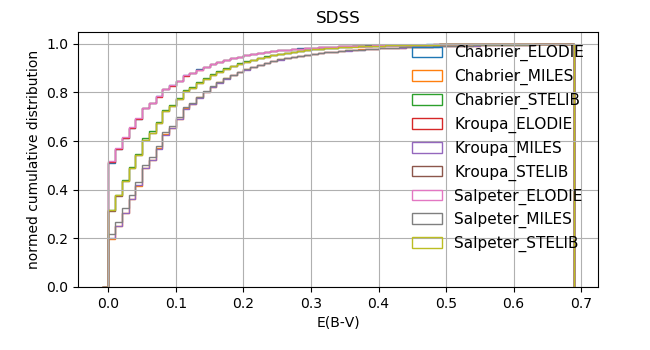
\includegraphics[width=4.5cm]{/home/comparat/software/firefly_explore/data/images/ebv/ebv_distribution_sdss.png}
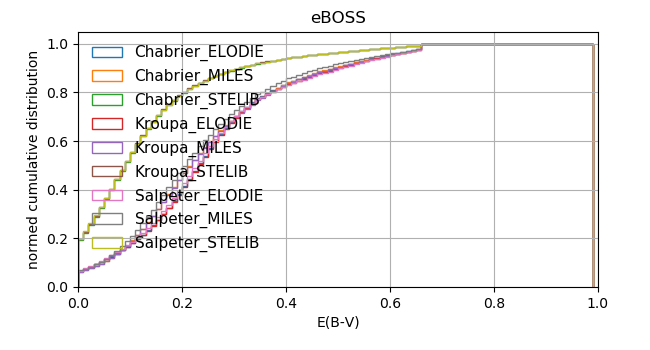
\includegraphics[width=4.5cm]{/home/comparat/software/firefly_explore/data/images/ebv/ebv_distribution_eboss.png}          
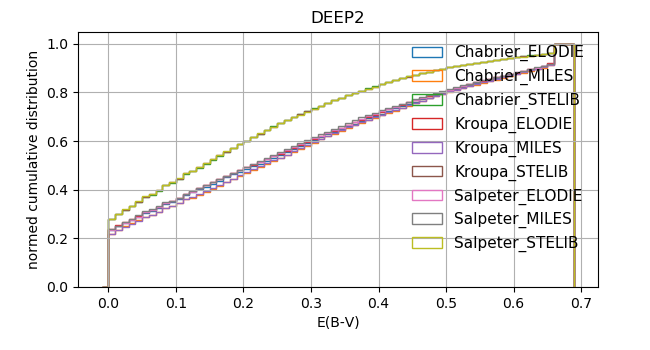
\includegraphics[width=4.5cm]{/home/comparat/software/firefly_explore/data/images/ebv/ebv_distribution_deep2.png} \\
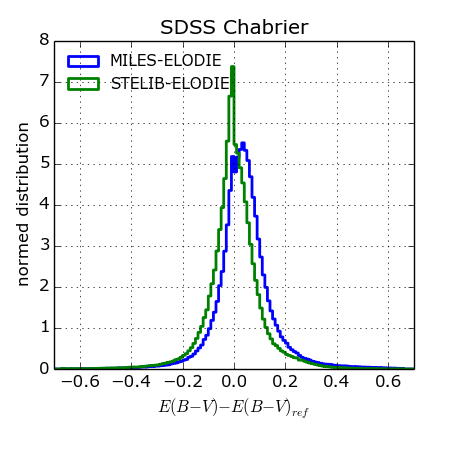
\includegraphics[width=4.5cm]{/home/comparat/software/firefly_explore/data/images/ebv/delta_EBV_distribution_sdssChabrier.png}
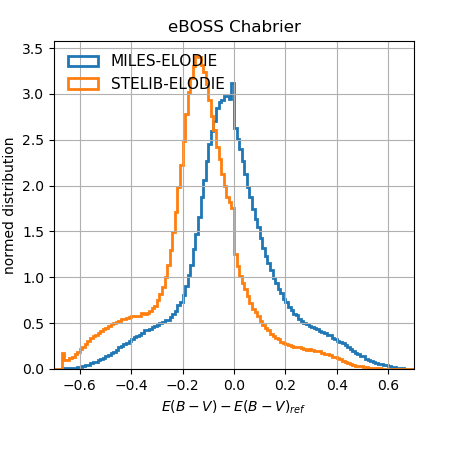
\includegraphics[width=4.5cm]{/home/comparat/software/firefly_explore/data/images/ebv/delta_EBV_distribution_ebossChabrier.png}
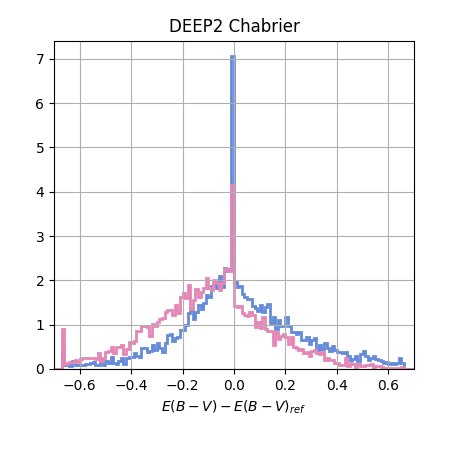
\includegraphics[width=4.5cm]{/home/comparat/software/firefly_explore/data/images/ebv/delta_EBV_distribution_deep2Chabrier.png}
% 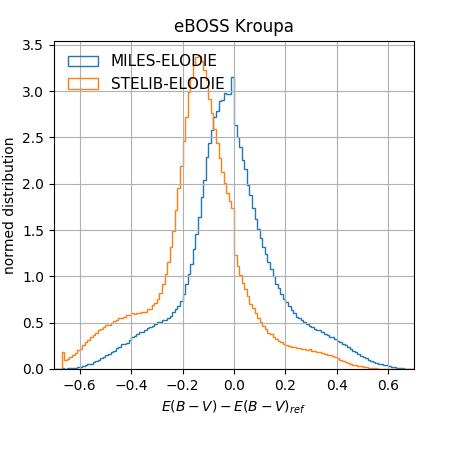
\includegraphics[width=4.5cm]{/home/comparat/software/firefly_explore/data/images/ebv/delta_EBV_distribution_ebossKroupa.png}
% 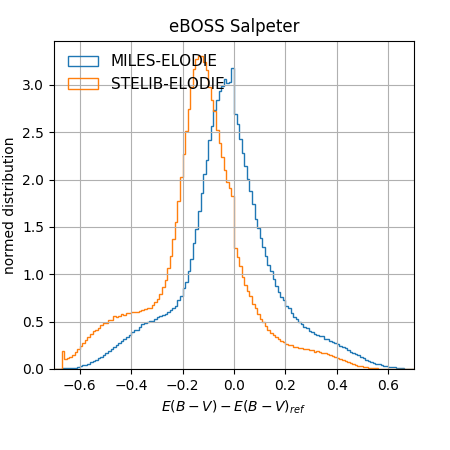
\includegraphics[width=4.5cm]{/home/comparat/software/firefly_explore/data/images/ebv/delta_EBV_distribution_ebossSalpeter.png} \\
% 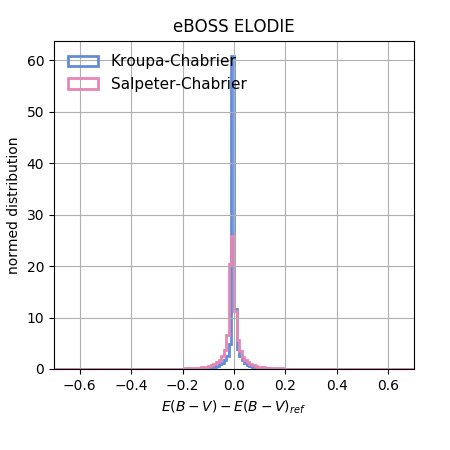
\includegraphics[width=4.5cm]{/home/comparat/software/firefly_explore/data/images/ebv/delta_EBV_distribution_ebossELODIE.png}
% 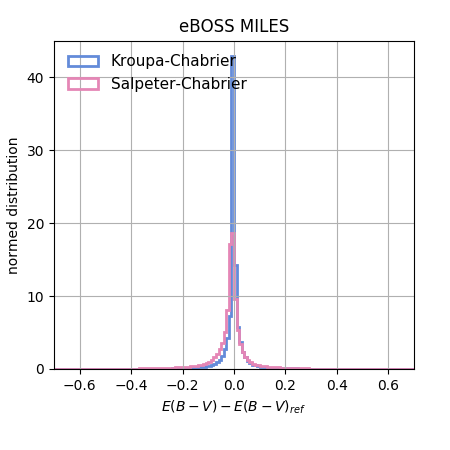
\includegraphics[width=4.5cm]{/home/comparat/software/firefly_explore/data/images/ebv/delta_EBV_distribution_ebossMILES.png}
% 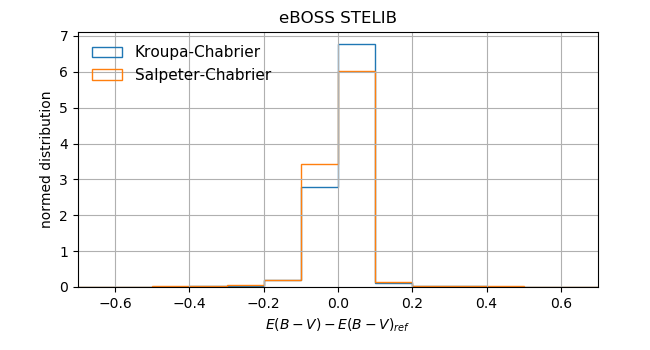
\includegraphics[width=4.5cm]{/home/comparat/software/firefly_explore/data/images/ebv/delta_EBV_distribution_ebossSTELIB.png}
\end{center}
\end{figure}


\subsubsection{Ages and metallicities sampled by the models}
We show in the figures below how each dataset 

\begin{figure}
\begin{center}
\caption{\label{fig:distributions:AZ} 
Age metallicity 2d-histograms for the SDSS (top row) eBOSS (middle row) and DEEP2 (ADD IT) data in the 3 library setups: columns ELODIE, MILES, STELIB for the Chabrier IMF. 
It shows how each library samples the age-metallicity plane. 
The differnces in occupation between surveys are driven by the redshift distribution in the samples.}
%, Kroupa and Salpeter.}  
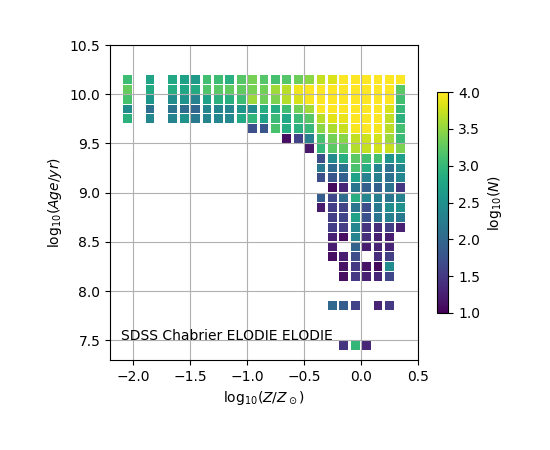
\includegraphics[height=4.5cm]{/home/comparat/software/firefly_explore/data/images/az/age_metallicity_Chabrier_ELODIE_sdss_04.png}
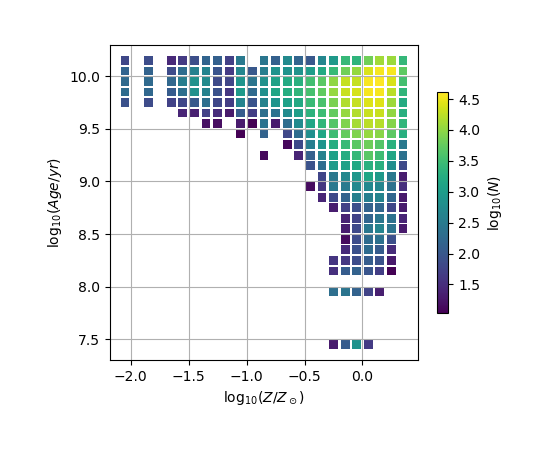
\includegraphics[height=4.5cm]{/home/comparat/software/firefly_explore/data/images/az/age_metallicity_Chabrier_MILES_sdss_04.png}
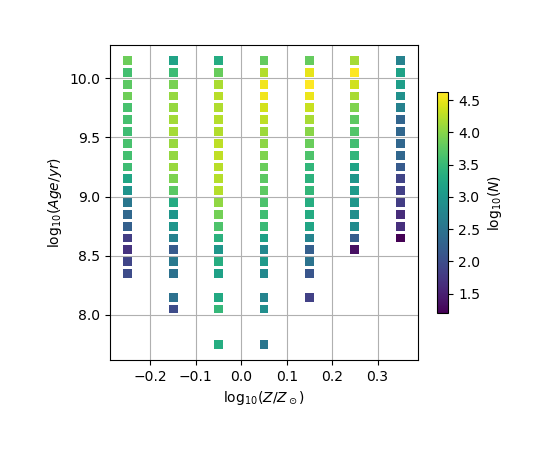
\includegraphics[height=4.5cm]{/home/comparat/software/firefly_explore/data/images/az/age_metallicity_Chabrier_STELIB_sdss_04.png}
% 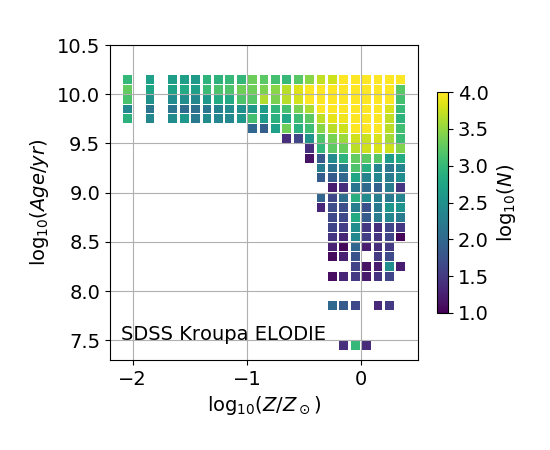
\includegraphics[height=4.5cm]{/home/comparat/software/firefly_explore/data/images/az/age_metallicity_Kroupa_ELODIE_sdss_04.png}
% 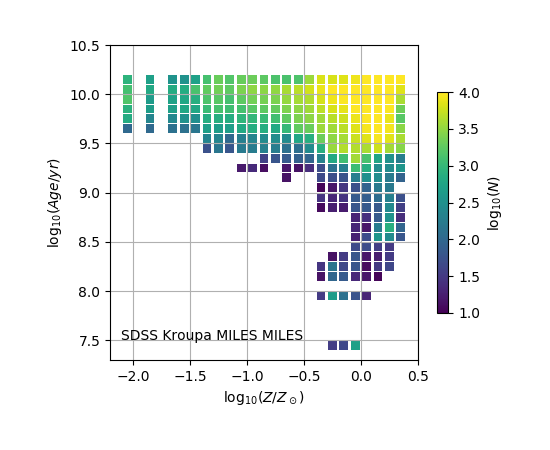
\includegraphics[height=4.5cm]{/home/comparat/software/firefly_explore/data/images/az/age_metallicity_Kroupa_MILES_sdss_04.png}
% 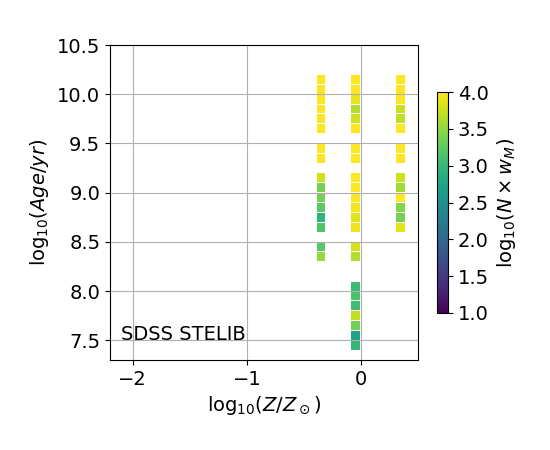
\includegraphics[height=4.5cm]{/home/comparat/software/firefly_explore/data/images/az/age_metallicity_Kroupa_STELIB_sdss_04.png}
% 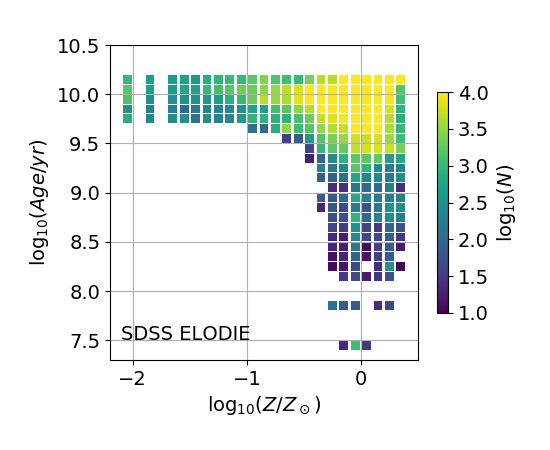
\includegraphics[height=4.5cm]{/home/comparat/software/firefly_explore/data/images/az/age_metallicity_Salpeter_ELODIE_sdss_04.png}
% 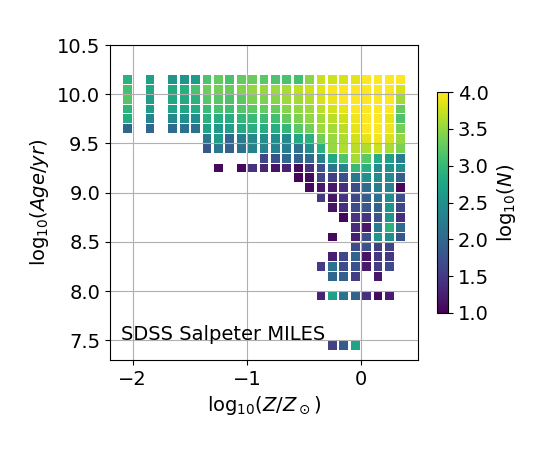
\includegraphics[height=4.5cm]{/home/comparat/software/firefly_explore/data/images/az/age_metallicity_Salpeter_MILES_sdss_04.png}
% 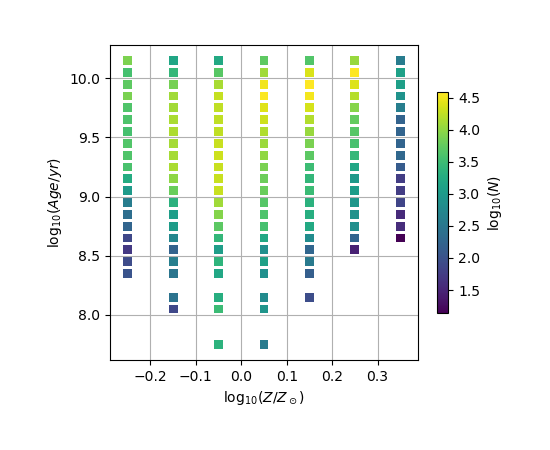
\includegraphics[height=4.5cm]{/home/comparat/software/firefly_explore/data/images/az/age_metallicity_Salpeter_STELIB_sdss_04.png}
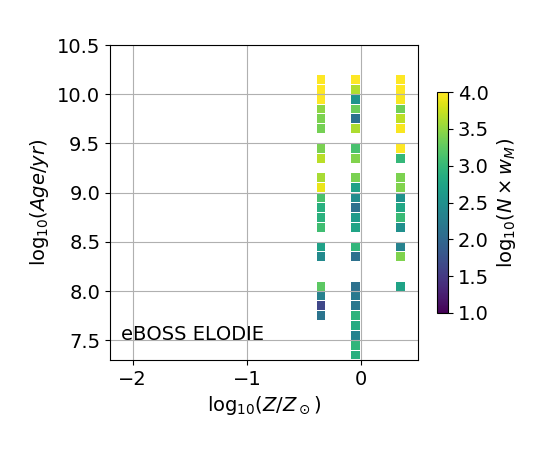
\includegraphics[height=4.5cm]{/home/comparat/software/firefly_explore/data/images/az/age_metallicity_Chabrier_ELODIE_eboss_04.png}
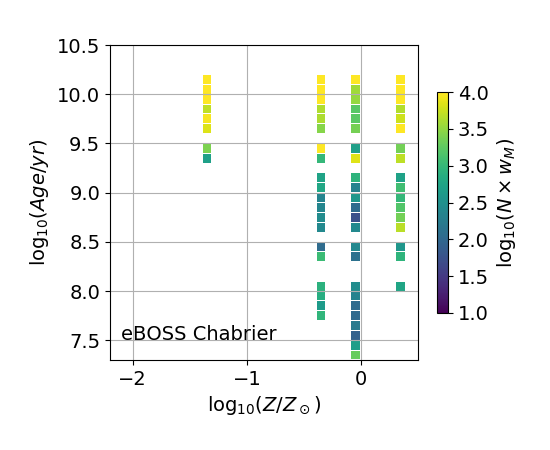
\includegraphics[height=4.5cm]{/home/comparat/software/firefly_explore/data/images/az/age_metallicity_Chabrier_MILES_eboss_04.png}
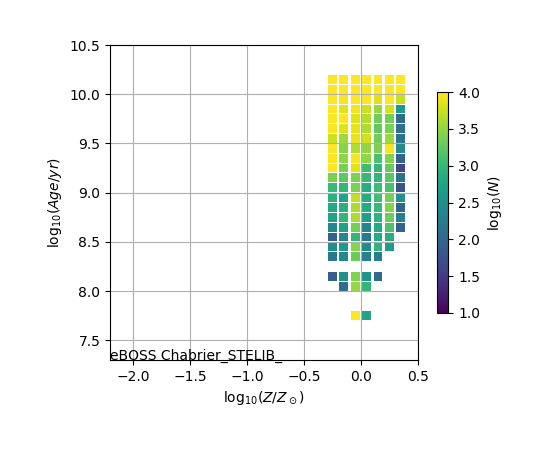
\includegraphics[height=4.5cm]{/home/comparat/software/firefly_explore/data/images/az/age_metallicity_Chabrier_STELIB_eboss_04.png}
% 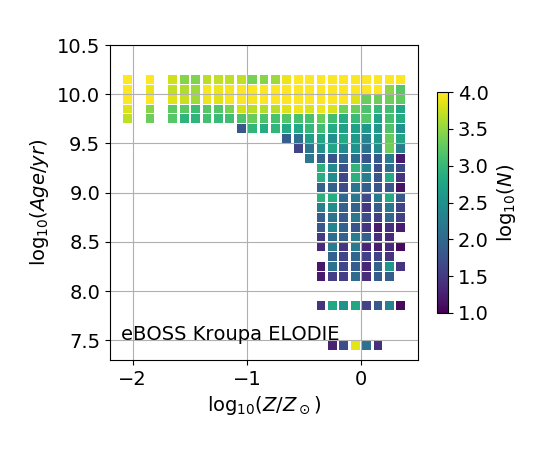
\includegraphics[height=4.5cm]{/home/comparat/software/firefly_explore/data/images/az/age_metallicity_Kroupa_ELODIE_eboss_04.png}
% 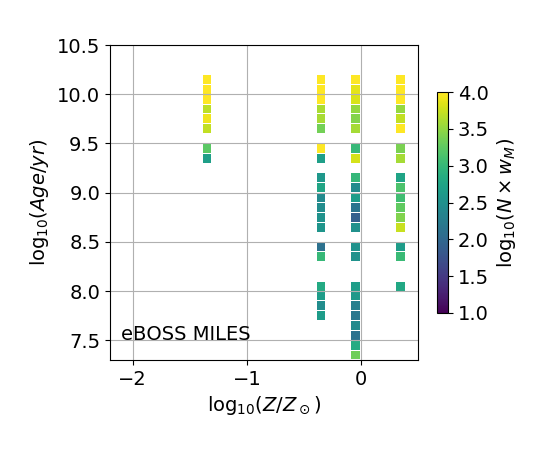
\includegraphics[height=4.5cm]{/home/comparat/software/firefly_explore/data/images/az/age_metallicity_Kroupa_MILES_eboss_04.png}
% 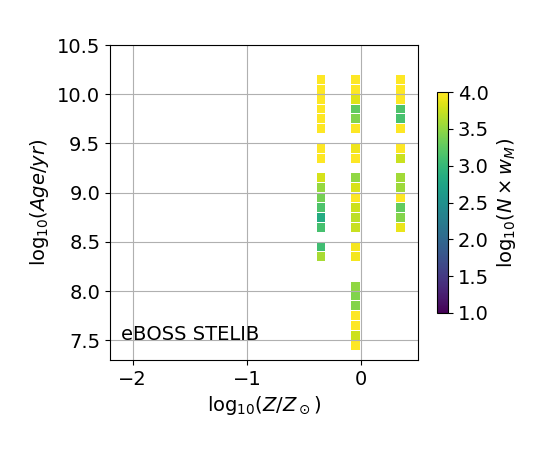
\includegraphics[height=4.5cm]{/home/comparat/software/firefly_explore/data/images/az/age_metallicity_Kroupa_STELIB_eboss_04.png}
% 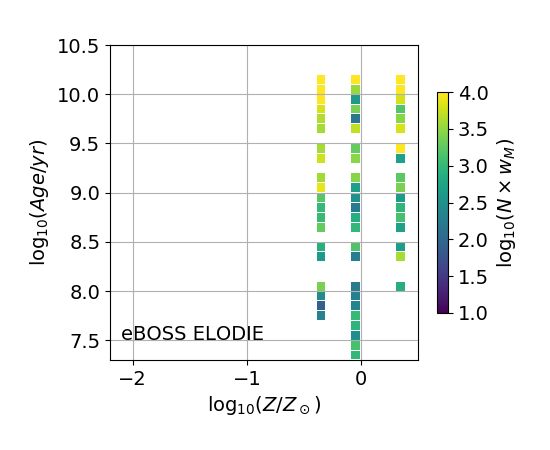
\includegraphics[height=4.5cm]{/home/comparat/software/firefly_explore/data/images/az/age_metallicity_Salpeter_ELODIE_eboss_04.png}
% 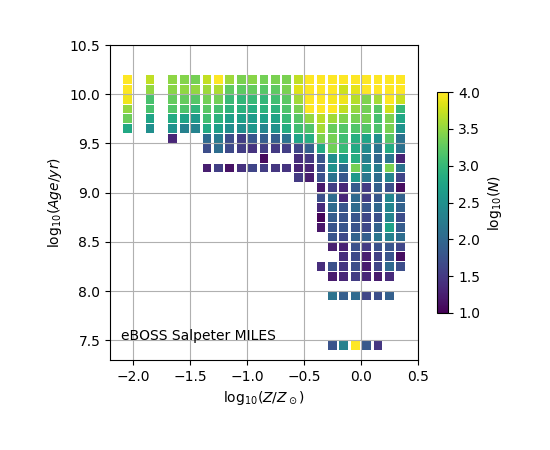
\includegraphics[height=4.5cm]{/home/comparat/software/firefly_explore/data/images/az/age_metallicity_Salpeter_MILES_eboss_04.png}
% 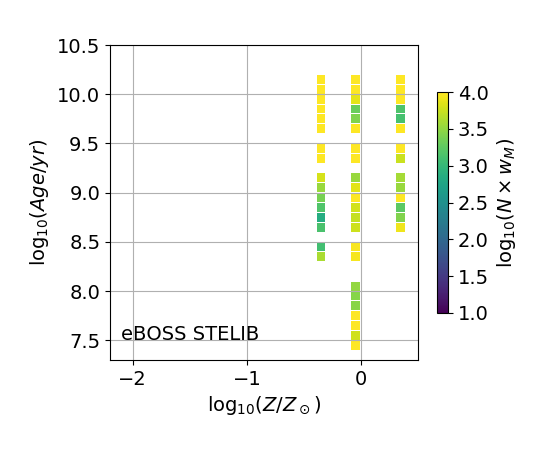
\includegraphics[height=4.5cm]{/home/comparat/software/firefly_explore/data/images/az/age_metallicity_Salpeter_STELIB_eboss_04.png}
\end{center}
\end{figure}
% 
% \begin{figure}
% \begin{center}
% \caption{\label{fig:distributions:AZ} 
% Age metallicity 2d-histograms for the SDSS data in the 9 setups: columns ELODIE, MILES, STELIB and rows Chabrier, Kroupa and Salpeter.}  
% \end{center}
% \end{figure}


\subsubsection{Stellar age}

Comment on the distributions.

In eBOSS data, assuming different stellar libraries, ages are boradly consistent, see Fig. \ref{fig:distributions:MwA} bottom plot. DO the same for SDSS and DEEP2.
%At fixed stellar library the ages determined are consistent.

\begin{figure}
\begin{center}
\caption{\label{fig:distributions:MwA} 
Normed cumulative distribution of the stellar parameters fitted: mass weighted age (left) light weighted (right).}  
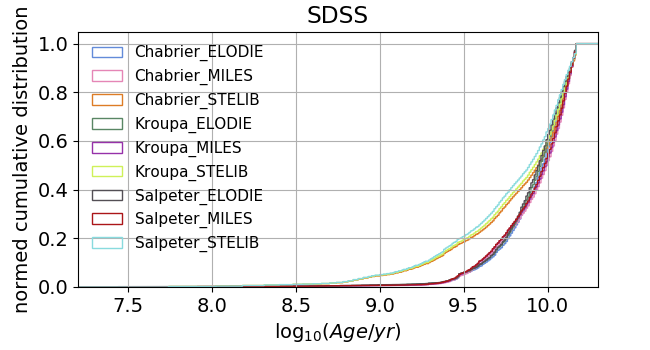
\includegraphics[height=4cm]{/home/comparat/software/firefly_explore/data/images/age_massW_distribution_sdss.png}
\includegraphics[height=4cm]{/home/comparat/software/firefly_explore/data/images/age_lightW_distribution_sdss.png}\\
\includegraphics[height=4cm]{/home/comparat/software/firefly_explore/data/images/age_massW_distribution_eboss.png}
\includegraphics[height=4cm]{/home/comparat/software/firefly_explore/data/images/age_lightW_distribution_eboss.png}\\
\includegraphics[height=4cm]{/home/comparat/software/firefly_explore/data/images/age_massW_distribution_deep2.png}
\includegraphics[height=4cm]{/home/comparat/software/firefly_explore/data/images/age_lightW_distribution_deep2.png}\\
\includegraphics[height=8cm]{comparison/delta_A_distribution_ebossChabrier.png}
\end{center}
\end{figure}

% \begin{figure}
% \begin{center}
% \caption{\label{fig:distributions:LwA} 
% Normed cumulative distribution of the stellar parameters fitted: light weighted age.}  
% \end{center}
% \end{figure}
% 
% \begin{figure}
% \begin{center}
% \caption{\label{fig:comparison:imfs:A} 
% Direct comparison of the light weighted stellar ages fitted $(M_1-M_{ref})/\sqrt{\sigma^2_{M_1}+\sigma^2_{M_{ref}}}$ where $\sigma$ are 1$\sigma$ errors for a fixed stellar library (ELODIE, left; STELIB, middle; MILES, right) varying the IMF. 
% If the obtained distribution follows a normal distribution depicted with the line 'N(0,1)' then measurements agree within errors. 
% At fixed stellar library the ages determined are consistent.}
% \includegraphics[height=8cm]{/home/comparat/software/firefly_explore/data/images/fixed_lib/delta_A_distribution_ebossELODIE.png}
% \includegraphics[height=8cm]{/home/comparat/software/firefly_explore/data/images/fixed_lib/delta_A_distribution_ebossSTELIB.png}
% \includegraphics[height=8cm]{/home/comparat/software/firefly_explore/data/images/fixed_lib/delta_A_distribution_ebossMILES.png}
% \end{center}
% \end{figure}

\subsection{Stellar metallicity}

The change in stellar library produces vast changes in metallicities.

\begin{figure}
\begin{center}
\caption{\label{fig:distributions:MwZ} 
Normed cumulative distribution of the stellar parameters fitted: mass weighted metallicity (left), light weighted metallicities (right).}  
\includegraphics[height=4cm]{/home/comparat/software/firefly_explore/data/images/metallicity_massW_distribution_sdss.png}
\includegraphics[height=4cm]{/home/comparat/software/firefly_explore/data/images/metallicity_lightW_distribution_sdss.png}    \\
\includegraphics[height=4cm]{/home/comparat/software/firefly_explore/data/images/metallicity_massW_distribution_eboss.png}
\includegraphics[height=4cm]{/home/comparat/software/firefly_explore/data/images/metallicity_lightW_distribution_eboss.png}     \\
\includegraphics[height=4cm]{/home/comparat/software/firefly_explore/data/images/metallicity_massW_distribution_deep2.png}
\includegraphics[height=4cm]{/home/comparat/software/firefly_explore/data/images/metallicity_lightW_distribution_deep2.png} \\
\includegraphics[height=8cm]{comparison/delta_Z_distribution_ebossChabrier.png}

\end{center}
\end{figure}
% 
% \begin{figure}
% \begin{center}
% \caption{\label{fig:distributions:LwZ} 
% Normed cumulative distribution of the stellar parameters fitted: light weighted metallicity.}  
% \end{center}
% \end{figure}
% % 
% \begin{figure}
% \begin{center}
% \caption{\label{fig:comparison:imfs:Z} 
% Direct comparison of the light weighted stellar metallicities fitted $(M_1-M_{ref})/\sqrt{\sigma^2_{M_1}+\sigma^2_{M_{ref}}}$ where $\sigma$ are 1$\sigma$ errors for a fixed stellar library (ELODIE, left; STELIB, middle; MILES, right) varying the IMF. 
% If the obtained distribution follows a normal distribution depicted with the line 'N(0,1)' then measurements agree within errors. 
% At fixed stellar library the metallicities determined are consistent.}
% \includegraphics[height=8cm]{/home/comparat/software/firefly_explore/data/images/fixed_lib/delta_Z_distribution_ebossELODIE.png}
% \includegraphics[height=8cm]{/home/comparat/software/firefly_explore/data/images/fixed_lib/delta_Z_distribution_ebossSTELIB.png}
% \includegraphics[height=8cm]{/home/comparat/software/firefly_explore/data/images/fixed_lib/delta_Z_distribution_ebossMILES.png}
% \end{center}
% \end{figure}


\subsection{Stellar mass}

Fig. \ref{fig:distributions:MS} shows the normed cumulative distribution of the stellar masses obtained.

\begin{figure}
\begin{center}
\caption{\label{fig:distributions:MS} 
Normed cumulative distribution of the stellar parameters fitted: stellar mass.}  
\includegraphics[height=8cm]{/home/comparat/software/firefly_explore/data/images/mass_distribution_sdss.png}
\includegraphics[height=8cm]{/home/comparat/software/firefly_explore/data/images/mass_distribution_eboss.png}
\includegraphics[height=8cm]{/home/comparat/software/firefly_explore/data/images/mass_distribution_deep2.png}
\end{center}
\end{figure}


\begin{figure}
\begin{center}
\caption{\label{fig:comparison:imfs:MS} 
Direct comparison of the stellar masses fitted $(M_1-M_{ref})/\sqrt{\sigma^2_{M_1}+\sigma^2_{M_{ref}}}$ where $\sigma$ are 1$\sigma$ errors for a fixed stellar library (ELODIE, left; STELIB, middle; MILES, right) varying the IMF. If the obtained distribution follows a normal distribution depicted with the line 'N(0,1)' then measurements agree within errors. 
Stellar masses are systematically different, as expected. Kroupa is systematically less massive than Chabrier than Salpeter.}
\includegraphics[height=8cm]{comparison/delta_M_distribution_ebossELODIE.png}
\includegraphics[height=8cm]{comparison/delta_M_distribution_ebossSTELIB.png}
\includegraphics[height=8cm]{comparison/delta_M_distribution_ebossMILES.png}
\end{center}
\end{figure}



\begin{figure*}
\begin{center}
\caption{\label{fig:comparison:library} 
Direct comparison of the stellar parameters fitted $(M_1-M_{ref})/\sqrt{\sigma^2_{M_1}+\sigma^2_{M_{ref}}}$ where $\sigma$ are 1$\sigma$ errors. The mass (left column), mass weighted age (middle column) and mass weighted metallicity (right column) for the Chabrier IMF varying the library used. 
If the obtained distribution follows a normal distribution depicted with the line 'N(0,1)' then measurements agree within errors. 
Ages are broadly consistent. 
Stellar masses and metallicities are not. 
With STELIB and MILES stellar mass and metallicity parameters obtained are systematically higher than with ELODIE. 
These systematic differences do not depend on the IMF.}  
\includegraphics[height=8cm]{comparison/delta_M_distribution_ebossChabrier.png}
% \includegraphics[height=8cm]{comparison/delta_A_distribution_ebossChabrier.png}
% \includegraphics[height=8cm]{comparison/delta_Z_distribution_ebossChabrier.png}

% \includegraphics[height=3cm]{comparison/delta_M_distribution_ebossSalpeter.png}
% \includegraphics[height=3cm]{comparison/delta_A_distribution_ebossSalpeter.png}
% \includegraphics[height=3cm]{comparison/delta_Z_distribution_ebossSalpeter.png}
\end{center}
\end{figure*}




\subsubsection{Star formation histories}
















\clearpage
\section{Results}
\label{sec:results}

% \begin{figure}
% \begin{center}
% \caption{\label{fig:error:pdf:SNR}Cumulative probability distribution function of the uncertainty on the stellar mass (Chabrier IMF) for different bins in median signal to noise ratio per pixel (MEDIAN\_SN\_ALL) for different libraries ELODIE (top), MILES (middle), STELIB (bottom). 
% Bin values are given on the plots.
% The largest uncertainties come from the ELODIE library and the smallest uncertainties from the STELIB library.
% Having a SNR larger than 2 per pixel guarantees an uncertainty smaller than 0.2 dex (at given IMF) in 90\% to 95\% of the cases.}

% \includegraphics[width=6.5cm]{plots/Chabrier_ELODIE__pdf_DELTA_logM_SNR_cumulative.jpg}

% \vspace*{-0.5cm}

% \includegraphics[width=6.5cm]{plots/Chabrier_MILES__pdf_DELTA_logM_SNR_cumulative.jpg}

% \vspace*{-0.5cm}

% \includegraphics[width=6.5cm]{plots/Chabrier_STELIB__pdf_DELTA_logM_SNR_cumulative.jpg}
% \end{center}
% \end{figure}

The SDSS+eBOSS specObjAll file contains (1,843,200 + 3,008,000 spectra) among which 950,705 + 1,765,156 are classified as galaxies. Are input for a fit 1,759,362 (99.6\%) + 948,259 (99.7\%) and 34,851 (DEEP2) spectra, see Table \ref{table:single:spectra}. The small fraction of missing data in SDSS is due to the fact that we only use the 26 runs and that serendipitously in stellar runs 103 and 104 some galaxies might have been mis-targeted. More than 95\% for SDSS and eBOSS see their output stellar mass constrained i.e. $0<M^*-\sigma_M<M^*+\sigma_M<10^{14} M_\odot$. The remaining 5\% have returned fitted parameters but they are consistent with a stellar mass of 0, thus calling these `unconstrained'. In DEEP2 the fraction of constrained fit is lower due to the lower signal to noise ratio of the data.
%We fit the M11 stellar population models using the \textsc{Firefly} software fitter to 1,618,192 (eBOSS) + 851,755 (SDSS) + 34,851 (DEEP2) = 2,504,798 spectra that were identified as galaxies by these surveys. 
For each spectrum we provide models of the continuum in up to 9 combinations of IMF and input model. 
This is the first full spectral fitting release of the BOSS+eBOSS high-redshift extension of SDSS which provide stellar population parameters. 
Previous work performing spectral fitting was based on a PCA approach \citep{2012MNRAS.421..314C} aimed at maximising the stellar mass determination, and the other stellar parameters were not provided.

In the next sections we discuss about the convergence of the fits (Sec. \ref{subsec:about:convergence}). 
Then, we measure the stellar mass function of \OII emitters in DEEP2.

\subsection{Accuracy in derived stellar mass}
\label{subsec:about:convergence}
In the case Chabrier+MILES, 80\% (70\%) of the SDSS (eBOSS) data, stellar masses are constrained to the 0.2 dex level. 
By `constrained', we mean that the statistical errors are small. 
Compared to previous studies on the SDSS data, based on spectrophotometry \citep[e.g.][]{Maraston2013}, the sample size of galaxies with stellar masses constrained to this level is increased by a factor of 2. 
Therefore we are gaining significant insight on the stellar population parameters. 
Parameters based on broad-band SEDs on the other hand could be calculated for all data as they are less dependent on the SNR of the spectroscopic data. 
For the DEEP2 data, due to the intrinsic faintness of the spectra and the much lower SNR of the continuum, we could tightly constrain the stellar mass for about 10\% of the sample.
Exact numbers are available in Table \ref{table:single:spectra}. 
The accuracy in constraining the fitted parameters is directly related to the signal to noise ratio measured in the spectrum, as mentioned in Sec. \ref{subsec:firefly:performances} and further discussed in Sec. \ref{subsec:stat:err}. 

Depending on initial setup, 87 to 97\% of the fits give constrained parameters for the SDSS+eBOSS data and between 50 and 60\% for the DEEP2 data. 
In SDSS+eBOSS, un-constrained fits are dominated by spectra with low signal to noise ratio and by some QSOs that were mis-classified as galaxies by the automated pipeline. % when the '\_NOQSO' option is used. 
In the DEEP2 data, the un-constrained fits are split into two components: low redshift galaxies for which the wavelength coverage of the spectra was not sufficient (the wavelength coverage of the observations does not contain the wavelength coverage of the model); very low signal to noise ratio in the continuum (emission line redshifts). 
In any case, the obtained sample is not a clean subset of the parent catalogs, rather it is a biased subsample of the parent catalogs.

\subsubsection{Statistical error on the stellar mass}
\label{subsec:stat:err}
The statistical uncertainty on the stellar mass is estimated using the full probability distribution function of the parameters derived during the fit. 
Variations between spectra are mainly driven by the average signal-to-noise per pixel in the spectra in the band where information is localized (roughly 3800-5500$\AA$). 

% The last row of panels of Fig. \ref{fig:mass:redshift} shows how the median signal to noise ratio in the $i$-band correlates with the statistical error derived on the estimated stellar mass. 
% At low redshift, we find that the SNR provided in the SDSS catalog is reliable and correlation comes in as expected. 
% Conversely at redshift higher than 0.5, the band of interest shifts into the $z$-band so that the correlation with the $i$-band seems to disappear. 
% Looking at this correlation with the SNR in the $z$-band, we find that the estimator is dominated by pixels contaminated by sky lines. The expected correlation is not present in the $z$-band, the plot is nearly the same as the one showed for the $i$-band. 
% A mentioned before, in future releases, we will provide a more robust estimators of the 'effective' SNR in the redder part of the spectrum, which will give the user a better handle on the convergence and sample selection. 
% This redshift effect set aside, the SNR when used conservatively ($>10$), still contains a useful information. 
%for a median SNR per pixel larger than 10, stellar masses are constrained to better than 0.2 dex in $>95\%$ of the cases. 
%For a median SNR per pixel larger than 1 (blue curves), stellar masses are constrained to better than 0.6 dex in $>95\%$ of the cases. 
%The stellar mass constraint degrades quickly when the median SNR is below 1, as one might expect. 
For spectra with large error on the stellar mass, one should be cautious, and combine this measurement with stellar masses (and other parameters in general) based on broad band magnitudes SED fitting \citep[e.g.][for the same galaxies]{Maraston2013}. 
In some sense, our new catalogs provide stellar masses with a better constrains for a subset of the complete sample SDSS+eBOSS.
%Yet, to be able to process a spectrum down to approx 1 is an amazing result, which will allow us to extend the same approach of spectral fitting at much higher redshifts. 
%So masses measured on spectra with SNR per pixel greater than 1 should be trusted. 

\subsubsection{Systematical biases and errors}

%There are systematic differences between the panels of Fig. \ref{fig:error:pdf:SNR}. 
We find that the average uncertainties on the stellar mass is systematically larger when comparing the M11-ELODIE results to the M11-STELIB ones. 
%Although the statistical error behave well, we see a systematic 0.2 dex difference in the stellar mass uncertainty. 
It should be noted as showed and fully discussed in \citet{Maraston_2011} that the ELODIE stellar library while allowing for a higher spectral resolution and a wider coverage in metallicity, covers a narrower wavelength range with respect to the STELIB library (up to $\sim 6800\AA$ vs $\sim 8000\AA$, respectively). 
The narrower wavelength is probably the reason why more solutions due to age/metallicity/dust degeneracy could be accommodated in the fit, hence degrading somewhat the constrain. 
A wider wavelength range usually allows for a more robust determination of the properties of galaxies, not surprisingly \citep[e.g.][]{2012MNRAS.422.3285P}. 
 
The other crucial systematic uncertainty on the stellar mass and on stellar mass functions is due to the assumptions of different stellar population models. 
It is discussed in depth by \citet{2016MNRAS.455.4122B}. 
They showed that for the same IMF, different assumptions on the adopted stellar population models and dust lead to different stellar masses and stellar mass functions. 
Different stellar population models cause up to 0.3 dex systematic differences. 
Different dust models cause up to 0.2 dex systematic differences.
Hence, stellar mass values available in different catalogues will show systematic differences. 
The catalogs presented here follow the 'starforming' flavour of the calculations by the Portsmouth group for the data release 12 (Maraston et al. 2013) and available at \url{http://www.sdss.org/dr14/spectro/galaxy_portsmouth}. 
We compared the stellar masses obtained in the previous and the current catalogs. 
We found the distribution normed by area of the quantity $|M_1-M_2|/\sqrt{\sigma^2_{M1}+\sigma^2_{M2}}$ where $M_1$ and $M_2$ are the DR12 and the DR14 versions of the stellar mass measurement to be very close to a normal distribution if using $2\sigma$ errors. 
If using $1\sigma$ errors, there is a some level of tension between the catalogs.  
%Four distributions are showed using the Kroupa IMF and the MILES or STELIB templates. Two curves are for galaxies with a redshift in agreement between DR12 and DR14 and 
However, when we consider the subset where galaxies have the same redshift (within 0.001) and the same E(B-V) (within 0.02), then the tension at $1\sigma$ disappears. 
Overall, agreement with its predecessor is very good.

% \subsubsection{Total mass vs. stellar mass}

% Using a sub sample of the SDSS plates and the `Chabrier-M11-MILES' setup, we estimate the mass correction due to stellar mass losses (the corresponding catalogs are available at www.icg.port.ac.uk/firefly and as additional catalogs, see Sec. \ref{subsec:alt:cat}). 
% For 54,117 galaxies older than 6 Gyr, the distribution of the correction to the stellar mass has quartiles with values Q1, Q2, Q3 = -0.007, 0.009, 0.03.
% For 100,621 galaxies with an age $3<$age/Gyr$<6$, we get Q1, Q2, Q3 = 0.001, 0.003, 0.026.
% For 44,560 galaxies with an age $1<$age/Gyr$<3$, we obtain Q1, Q2, Q3 = -0.004, 0.0007, 0.005.
% For 3,711 galaxies with an age age/Gyr$<1$, the quartiles are Q1, Q2, Q3 = -0.012, 0.001, 0.018.
% As expected, the older the stellar population are more strongly affected \citep[e.g][]{1998MNRAS.300..872M,Maraston2005a}. 
% All in all, the variation between these catalogues is small: $<0.03$ dex with dependence on age. 
% For future SDSS releases (starting with DR15) we shall include all types of mass output in the default run.

% \begin{figure}
% \begin{center}
% \caption{\label{fig:comparison:previous:catalog}
% Area normed histogram of the difference between stellar masses weighted by their relative uncertainty (top panel) and twice the relative uncertainty (bottom panel). Agreement is generally good within 2 $\sigma$. 
% \includegraphics[width=8cm]{plots/comparison_firefly_portsmouthSF.png}
% \includegraphics[width=8cm]{plots/comparison_firefly_portsmouthSF_error_multiplied_by_2.png}
% \end{center}
% \end{figure}

\subsubsection{Overlap between SDSS, eBOSS and DEEP2}
There are galaxies in common which were observed by both SDSS and DEEP2, precisely 64 (493) galaxies were observed by both DEEP2 and SDSS (eBOSS). 
Among these, 31 (261) have redshift values that agree within $|z_{DEEP2}-z_{SDSS (eBOSS)}|<0.0005$. 
3 (31) galaxies have a stellar mass constrained within $\pm0.2$ dex. 
For these 3+31 galaxies, the masses measured agree within errors. 

\subsection{Stellar mass function sampled by emission line galaxies in DEEP2}
\label{subsec:smf:elg}
How emission line galaxies populate the cosmic web is a hot topic in cosmology nowadays \citep{favole_2015_elg,2017MNRAS.472..550F,raichoor_2017MNRAS.471.3955R,2017arXiv170807628G}. 
To characterize how emission line galaxies are related to the overall galaxy population, we project the DEEP2 observed stellar mass function in the redshift range $0.83<z<1.03$ for three \OII luminosity threshold, $\log_{10}($L[\OII]$)>41.8$, 42 and 42.2, see Fig.  \ref{fig:LF:sampling}. 
It is known that there is scatter in SFR at fixed mass and that the \OII -- SFR relation also has scatter. 
Therefore we do not expect to find that only a narrow range of masses is populated by the strongest \OII emitters.
Indeed, the distributions we find are quite broad, covering the stellar mass range $10^9<M/M_{\odot}<10^{11.5}$. 
More interestingly, these distributions are quite flat and their shape do not seem to depend on the luminosity threshold. 
Similar distributions were found in \citet{raichoor_2017MNRAS.471.3955R}. 
Given that the DEEP2 sample is complete for the \OII luminosity limits applied, we  conclude that up to $z=1.5$ there is no preferred host galaxy mass (in the range $10^9<M/M_{\odot}<10^{11.5}$) to find a strong \OII emission.

Recently, a broad range of properties of ELGs was predicted by the model presented in \citet{2017arXiv170807628G}. 
In our data, it seems that massive galaxies are selected as \OII emitters, something that was not expected from that model. 
This discrepancy might be related to the treatment of the dust in the model, although a further detailed analysis will be needed to understand better this very interesting puzzle.

The broad distribution in stellar mass means that studying stacked spectra of galaxies selected by emission line luminosity thresholds will result in a statement about their mean stellar populations, that is unlikely to capture the variety of galaxies constituting the emission line galaxy population.
Put differently, ELG stacks might not capture how diverse the ELG population actually is.  
This happens also because the light of emission-line selected galaxies is dominated by their latest generation of stars, which overshine the underlying structure of older stellar populations \citep[known as the 'iceberg effect'][]{2010MNRAS.407..830M}. 

\begin{figure}
\begin{center}
\includegraphics[type=png,ext=.png,read=.png,height=8cm]{plots/all_contour_SMF_raw_41_8_0_83_z_1_03}
\label{fig:LF:sampling}
\caption{Stellar mass function as measured in the DEEP2 \OII emitter sample in the redshift range $0.83<z<1.03$ (considering all combinations of IMF and libraries). 
We show the stellar mass function is sampled by the \OII emitters for different thresholds in $\log_{10}($L\OII$)$ luminosity 41.8, 42 and 42.2.}  
\end{center}
\end{figure}

\section{Summary and future releases}

We provide the stellar population properties as obtained by full spectral fitting of models to the observed spectra for SDSS DR14 galaxies, including their high-z extensions (eBOSS), and for the DEEP2 survey. 
Compared to previous releases, this one doubles the number of galaxies with a tightly constrained stellar mass parameter.
Thanks to the high performance computing environment "SCIAMA" at the University of Portsmouth, we could create models of the continuum for nine configurations of IMF and stellar libraries for about 2.7 million galaxies. 
This catalog is the continuation of the Portsmouth SDSS galaxy property catalogs, which were using the spectroscopic redshift combined with the broad-band photometry.
%Ours is the first release of this kind pushed down to very low SNR (SNR$\sim$1). 
To do so, we adopted the newly released \textsc{Firefly} fitting code coupled with the stellar population  models by \citet{Maraston_2011}. This combination has improved the precision of derived parameters. In particular, the stellar mass for SDSS galaxies is obtained with a precision of about 0.2 dex for a given IMF, when SNR$>20$. 
This shows that beyond providing an accurate redshift measurement and thus an accurate distance, there is large amount of valuable information in the spectra to help further constrain the stellar population history. 
%We explored the observed stellar mass function probed by SDSS, eBOSS and DEEP2 for galaxies with $0.2<z<0.8$, setting a strict lower limit to them. 

We explore for the first time the stellar population models of DEEP2 emission line galaxies and find that these galaxies span a variety of properties, which is in broad agreement with predictions of the state-of-the-art semi-analytical models. In particular, DEEP2 galaxies selected by their [OII] luminosity in the redshift range 0.83<z<1.03, have stellar masses with a constant number density in the range $10^9<M(M_{\odot})<10^{11.5}$.

Ongoing \textsc{firefly} developments expected for the next SDSS public release (DR16 onwards) are:
\begin{itemize}
\item A plugin to the SDSS webapp\footnote{\url{https://dr14.sdss.org/optical/spectrum/view}} to access interactively the continuum models.
\item Emission line measurements on the residuals.
\item An AGN mode to \textsc{firefly} to allow for fitting all the pixels of AGN spectra \citep[e.g.][]{2017MNRAS.472.4051C}.
\end{itemize}

There are a variety of science cases that will be explored in depth in upcoming companion papers. 
 
\section{Acknowledgements}
JC thanks the \textsc{firefly} team for the team work and this milestone ! 
We all thank Gary Burton for his superb help and technical support with the SCIAMA machine, and Anne-Marie Weijmans for her guidance through the VAC emission.

VGP acknowledges support from the University of Portsmouth through the Dennis Sciama Fellowship award. 
Numerical computations were done on the SCIAMA High Performance Compute cluster which is supported by the ICG, SEPNet and the University of Portsmouth. 
This research used resources of the National Energy Research Scientific Computing Center, a DOE Office of Science User Facility supported by the Office of Science of the U.S. 
Department of Energy under Contract No. DE-AC02-05CH11231. 
This work has benefited from the publicly available programming language {\sc python}.

Funding for the Sloan Digital Sky Survey IV has been provided by the Alfred P. Sloan Foundation, the U.S. Department of Energy Office of Science, and the Participating Institutions. SDSS acknowledges support and resources from the Center for High-Performance Computing at the University of Utah. The SDSS web site is www.sdss.org.

SDSS is managed by the Astrophysical Research Consortium for the Participating Institutions of the SDSS Collaboration including the Brazilian Participation Group, the Carnegie Institution for Science, Carnegie Mellon University, the Chilean Participation Group, the French Participation Group, Harvard-Smithsonian Center for Astrophysics, Instituto de Astrof\'{i}sica de Canarias, The Johns Hopkins University, Kavli Institute for the Physics and Mathematics of the Universe (IPMU) / University of Tokyo, Lawrence Berkeley National Laboratory, Leibniz Institut für Astrophysik Potsdam (AIP), Max-Planck-Institut für Astronomie (MPIA Heidelberg), Max-Planck-Institut für Astrophysik (MPA Garching), Max-Planck-Institut für Extraterrestrische Physik (MPE), National Astronomical Observatories of China, New Mexico State University, New York University, University of Notre Dame, Observatório Nacional / MCTI, The Ohio State University, Pennsylvania State University, Shanghai Astronomical Observatory, United Kingdom Participation Group, Universidad Nacional Autónoma de México, University of Arizona, University of Colorado Boulder, University of Oxford, University of Portsmouth, University of Utah, University of Virginia, University of Washington, University of Wisconsin, Vanderbilt University, and Yale University.

\bibliographystyle{aa}
\bibliography{biblio}

\appendix


\section{Observed stellar mass function probed by SDSS, eBOSS and DEEP2}
\label{subsec:sdss:stellarmassdensity}

The galaxy stellar mass function and its evolution with redshift is a crucial property to perform galaxy formation and evolution studies \citep{2006ApJ...651..120B,2010A&A...523A..13P,Maraston2013,Ilbert2013SMF,2016MNRAS.455.4122B,2017MNRAS.466..228E}. 
The study of this function requires large numbers of galaxies hence usually $\sim M^{*}$ from broad-band photometry is adopted. 
Here we show - without aiming at performing a full scientific analysis - what we obtain for the galaxy mass function when using our results based on spectral fitting rather than broad-band photometry, and for three different datasets in two redshift bins.

We consider stellar masses constrained to better than 0.2 dex based on the Chabrier IMF for the three libraries ELODIE, STELIB and MILES. 
For eBOSS galaxies, we consider the area covered to be 10,000 deg2; for SDSS 7,900 deg2 and for DEEP2 0.5 deg2 (low redshift) or 2.78 deg2 (high redshift).
For SDSS and eBOSS each galaxy represents itself only, no weighting other than the area is applied. 
We do not correct for the eventual incompletenesses present in the SDSS and eBOSS data. 
For DEEP2, we use the statistical weights from \citet{Comparat2016LFs}. These weights correct from the target selection algorithm used in DEEP2 and allow the recovery of the correct galaxy density as a function of redshift and magnitude. 
For each catalog (3 surveys x 3 libraries), we estimate the observed stellar mass function (OSMF) and its Poisson error (cosmic variance is not taken into account). 
Then, per survey, we compute the median of the three measurements (3 libraries) and the minimum and maximum of the three measurements (with only Poisson errors considered). 
The OSMF obtained constitutes a robust a lower limit to the stellar mass function. 
Indeed because we use only stellar masses that are tightly constrained, we are certain that at least this density of stellar mass exists in galaxies.

We compare our results with the stellar mass functions obtained in COSMOS \citet{Ilbert2013SMF} and in BOSS \citep{Maraston2013}. 
This COSMOS stellar mass function is based on a $K$-band selected sample that is known to be biased at low redshift as it misses a fraction of the massive star-forming galaxy population i.e. at the high mass end our measurements are expected to be above that of COSMOS. 
We show the results in two redshift bins: $0.2<z<0.5$, $0.5<z<0.8$, see Fig. \ref{fig:smf:all}. 
We see how each sample (DEEP2, SDSS, eBOSS), considering only the tightly constrained stellar masses, is related to the bulk of the galaxy population depicted by the COSMOS and BOSS stellar mass functions. 
The comparison with \citet{Maraston2013} (purple line on the Figure) shows the level of incompleteness we have due to our selection on the error on the stellar mass. 
%These qualitative statements are in agreement with the measurements from \citep{Maraston2013,2016MNRAS.455.4122B}, where completeness is corrected for.

% Have you built the model lines from the lightcone? If so, the
% > underlying model is GP14,https://arxiv.org/abs/1309.7057 [65].
% > 
% > If thats the case, youll need to correct the IMF from Kennicut to
% > Chabrier (you can use the tables in
% > Lacey+16:http://adsabs.harvard.edu/abs/2016MNRAS.462.3854L [66].
% > 

\begin{figure}
\begin{center}
\includegraphics[height=8cm]{plots/firefly_SMF_BOSS_0_2_z_0_5.png}
\includegraphics[height=8cm]{plots/firefly_SMF_BOSS_0_5_z_0_8.png}
%\includegraphics[type=jpg,ext=.jpg,read=.jpg,height=8cm]{plots/firefly_SMF_BOSS_0_8_z_1_1}
\caption{\label{fig:smf:all}Stellar mass function measured on SDSS, eBOSS and DEEP2 samples containing only tightly constrained stellar masses. Two redshift bins $0.2<z<0.5$, $0.5<z<0.8$ show how each survey spans the stellar mass function. For comparison, we added the \citet{Ilbert2013SMF} model (green, they have the exact same redshift bins) and the BOSS SMF from \citet{Maraston2013}, their mean measurement is at redshift 0.5 (magenta line).}
\end{center}
\end{figure}


\section{Warning about fits with unconstrained parameters}

We would like to warn the future users about fits that led to unconstrained age, mass or metallicity parameters. 
Indeed for every spectrum, firefly provides an answer and the full pdf of each parameter. But sometimes, the pdf is so large that the uncertainties are as large as the parameters space itself. 
In such cases the value output should not be trusted. 
On Fig. \ref{fig:firefly:output:plate:unconstrained} we show such an example where the stellar mass parameter deduced with the MILES libraries are consistent with 0 whereas with STELIB or ELODIE, the stellar masses obtained have a smaller error. 

\section{Large figures and tables}


\begin{table*}
\begin{center}
\caption{\label{ref:table:sdss:src:firefly}SDSS division of the data per source type. Ordered by decreasing number of galaxies (third column). 
The second column, 'N', gives the number of spectra labeled under this sourcetype. 
The third column, 'N galaxies', gives the number of spectra considered as galaxies and their fraction relatively to the second column. 
The fourth gives, 'SNR ALL$>0$', the number of spectra considered as galaxies with a positive median SNR over its spectrum. We consider this column as the reference sample to be fitted by \textsc{firefly}, hence the 100\%. 
The fifth column, 'firefly constrained', gives the fraction of constrained fits and their fraction relative to the reference sample (column 4). 
For the Galaxy sourcetype (first line), it is very high at $810540/829464 \sim 97.7\%$. 
The last two columns, '$\sigma_{\log_M}<0.4$' ('$\sigma_{\log_M}<0.2$'), give the fraction of fits that have a stellar mass constrained within 0.4 (0.2) dex. 
It is around 80\% for the GALAXY and QA sourcetype. 
%The completeness is much lower for other sourcetypes.
}
\begin{tabular}{c rrr rrr rrrrrrrrrrrrrr}
\hline \hline
sourcetype & N & \multicolumn{2}{c}{N galaxies} & \multicolumn{2}{c}{SNR ALL$>0$} & \multicolumn{2}{c}{firefly constrained} & \multicolumn{2}{c}{$\sigma_{\log_M}<0.4$} & \multicolumn{2}{c}{$\sigma_{\log_M}<0.2$} \\ 
 & N & N & \% & N & \% & N & \% & N & \% & N & \%  \\ 
\hline 
GALAXY & 858244 & 829464 & 96 & 829464 & 100 & 810540 & 97 & 794149 & 95 & 673690 & 81 \\ 
NONLEGACY & 294745 & 75154 & 25 & 74899 & 100 & 68906 & 92 & 57586 & 76 & 33134 & 44 \\ 
QSO & 168563 & 22724 & 13 & 22724 & 100 & 19803 & 87 & 15252 & 67 & 8167 & 35 \\ 
QA & 20408 & 14608 & 71 & 14608 & 100 & 14286 & 97 & 13919 & 95 & 11630 & 79 \\ 
SERENDIPITY\_FIRST & 7526 & 4163 & 55 & 4163 & 100 & 3953 & 95 & 3576 & 85 & 2249 & 54 \\ 
ROSAT\_D & 7057 & 1704 & 24 & 1704 & 100 & 1642 & 96 & 1350 & 79 & 739 & 43 \\ 
SERENDIPITY\_DISTANT & 4911 & 251 & 5 & 251 & 100 & 221 & 88 & 146 & 58 & 68 & 27 \\ 
SERENDIPITY\_BLUE & 22871 & 70 & 0 & 70 & 100 & 54 & 77 & 31 & 44 & 12 & 17 \\ 
STAR\_WHITE\_DWARF & 2290 & 32 & 1 & 32 & 100 & 26 & 81 & 16 & 50 & 10 & 31 \\ 
SERENDIPITY\_MANUAL & 68 & 27 & 39 & 27 & 100 & 25 & 92 & 20 & 74 & 14 & 51 \\ 
STAR\_CARBON & 3458 & 22 & 0 & 22 & 100 & 20 & 90 & 15 & 68 & 9 & 40 \\ 
REDDEN\_STD & 15363 & 13 & 0 & 13 & 100 & 11 & 84 & 10 & 76 & 8 & 61 \\ 
STAR\_BHB & 14230 & 12 & 0 & 12 & 100 & 9 & 75 & 7 & 58 & 4 & 33 \\ 
STAR\_PN & 14 & 8 & 57 & 8 & 100 & 6 & 75 & 0 & 0 & 0 & 0 \\ 
SERENDIPITY\_RED & 2771 & 2 & 0 & 2 & 100 & 1 & 50 & 0 & 0 & 0 & 0 \\ 
HOT\_STD & 3413 & 2 & 0 & 2 & 100 & 2 & 100 & 2 & 100 & 1 & 50 \\ 
SPECTROPHOTO\_STD & 15366 & 1 & 0 & 1 & 100 & 1 & 100 & 1 & 100 & 1 & 100 \\ 
STAR\_BROWN\_DWARF & 560 & 1 & 0 & 1 & 100 & 0 & 0 & 0 & 0 & 0 & 0 \\ 
STAR\_CATY\_VAR & 6853 & 1 & 0 & 1 & 100 & 1 & 100 & 1 & 100 & 0 & 0 \\ 
SKY & 61967 & 0 & 0 & 0 & 100 & 0 & 0 & 0 & 0 & 0 & 0 \\ 
STAR\_SUB\_DWARF & 1226 & 0 & 0 & 0 & 100 & 0 & 0 & 0 & 0 & 0 & 0 \\ 
STAR\_RED\_DWARF & 14496 & 0 & 0 & 0 & 100 & 0 & 0 & 0 & 0 & 0 & 0 \\ 
\hline
\end{tabular}
\end{center}
\end{table*}

\begin{center}
\begin{longtable}{c rrr rrr rrrrrrrrrrrrrr}
\caption{\label{ref:table:boss:src:firefly} Same as Table \ref{ref:table:sdss:src:firefly} for eBOSS.}\\
\hline \hline
source type & N & \multicolumn{2}{c}{N galaxies} & \multicolumn{2}{c}{SNR ALL$>0$} & \multicolumn{2}{c}{firefly constrained} & \multicolumn{2}{c}{$\sigma_{\log_M}<0.4$} & \multicolumn{2}{c}{$\sigma_{\log_M}<0.2$} \\ 
 & N & N & \% & N & \% & N & \% & N & \% & N & \%  \\ 
\hline 
\endfirsthead

\caption{continued.}\\
\hline \hline
source type & N & \multicolumn{2}{c}{N galaxies} & \multicolumn{2}{c}{SNR ALL$>0$} & \multicolumn{2}{c}{firefly constrained} & \multicolumn{2}{c}{$\sigma_{\log_M}<0.4$} & \multicolumn{2}{c}{$\sigma_{\log_M}<0.2$} \\ 
 & N & N & \% & N & \% & N & \% & N & \% & N & \%  \\ 
\hline 
\endhead

\hline \multicolumn{3}{|r|}{{Continued on next page}} \\ \hline
\endfoot

\hline \hline
\endlastfoot
LRG & 1579529 & 1479496 & 93 & 906577 & 100 & 887235 & 97 & 769382 & 84 & 546392 & 60 \\ 
QSO & 645501 & 116243 & 18 & 61892 & 100 & 43481 & 70 & 30035 & 48 & 12669 & 20 \\ 
SEQUELS\_TARGET & 100810 & 38871 & 38 & 38871 & 100 & 36251 & 93 & 26190 & 67 & 11253 & 28 \\ 
SPIDERS\_RASS\_CLUS & 10623 & 10433 & 98 & 2573 & 100 & 2555 & 99 & 2530 & 98 & 2279 & 88 \\ 
WISE\_COMPLETE & 10019 & 9113 & 91 & 0 & 100 & 0 & 0 & 0 & 0 & 0 & 0 \\ 
HIZ\_LRG & 9541 & 7463 & 78 & 0 & 100 & 0 & 0 & 0 & 0 & 0 & 0 \\ 
RM\_TILE1 & 11270 & 7342 & 65 & 7342 & 100 & 6351 & 86 & 5579 & 76 & 3075 & 41 \\ 
WISE\_BOSS\_QSO & 15851 & 6664 & 42 & 4512 & 100 & 3732 & 82 & 3182 & 70 & 1957 & 43 \\ 
RM\_TILE2 & 30331 & 6475 & 21 & 6475 & 100 & 4586 & 70 & 3391 & 52 & 1847 & 28 \\ 
BRIGHTGAL & 5565 & 5361 & 96 & 3541 & 100 & 3403 & 96 & 3370 & 95 & 3292 & 93 \\ 
ELG\_TEST1 & 7200 & 4525 & 62 & 0 & 100 & 0 & 0 & 0 & 0 & 0 & 0 \\ 
ELG1\_EBOSS & 4741 & 3616 & 76 & 0 & 100 & 0 & 0 & 0 & 0 & 0 & 0 \\ 
SN\_GAL1 & 4042 & 3502 & 86 & 3496 & 100 & 3345 & 95 & 2797 & 80 & 1900 & 54 \\ 
ELG\_DECALS\_TEST1 & 5356 & 3423 & 63 & 0 & 100 & 0 & 0 & 0 & 0 & 0 & 0 \\ 
SEQUELS\_ELG & 4217 & 3059 & 72 & 3059 & 100 & 2763 & 90 & 1290 & 42 & 175 & 5 \\ 
BLUE\_RADIO & 2920 & 2874 & 98 & 1791 & 100 & 1744 & 97 & 1687 & 94 & 1390 & 77 \\ 
QSO\_VAR\_LF & 9069 & 2507 & 27 & 2313 & 100 & 1888 & 81 & 1164 & 50 & 456 & 19 \\ 
QSO\_WISE\_FULL\_SKY & 8271 & 2482 & 30 & 1247 & 100 & 1037 & 83 & 856 & 68 & 408 & 32 \\ 
QSO\_VAR\_SDSS & 22752 & 2297 & 10 & 1527 & 100 & 1205 & 78 & 855 & 56 & 339 & 22 \\ 
SEQUELS\_ELG\_LOWP & 2982 & 2269 & 76 & 2269 & 100 & 2025 & 89 & 922 & 40 & 153 & 6 \\ 
FAINT\_ELG & 2699 & 2235 & 82 & 2235 & 100 & 1942 & 86 & 855 & 38 & 85 & 3 \\ 
QSO1\_REOBS & 16021 & 2153 & 13 & 443 & 100 & 242 & 54 & 142 & 32 & 41 & 9 \\ 
CLUSTER\_MEMBER & 2072 & 2056 & 99 & 577 & 100 & 568 & 98 & 565 & 97 & 521 & 90 \\ 
LRG\_ROUND3 & 2486 & 2032 & 81 & 0 & 100 & 0 & 0 & 0 & 0 & 0 & 0 \\ 
GAL\_NEAR\_QSO & 2037 & 1954 & 95 & 1140 & 100 & 1111 & 97 & 990 & 86 & 670 & 58 \\ 
TDSS\_B & 18880 & 1734 & 9 & 489 & 100 & 410 & 83 & 358 & 73 & 225 & 46 \\ 
ELG & 3479 & 1650 & 47 & 409 & 100 & 348 & 85 & 153 & 37 & 25 & 6 \\ 
S82X\_TILE1 & 2775 & 1608 & 57 & 0 & 100 & 0 & 0 & 0 & 0 & 0 & 0 \\ 
QSO\_SUPPZ & 4839 & 1512 & 31 & 1213 & 100 & 825 & 68 & 749 & 61 & 578 & 47 \\ 
STRIPE82BCG & 1407 & 1388 & 98 & 1380 & 100 & 1359 & 98 & 1302 & 94 & 1122 & 81 \\ 
QSO\_WISE\_SUPP & 3992 & 1065 & 26 & 1065 & 100 & 945 & 88 & 771 & 72 & 366 & 34 \\ 
SPIDERS\_RASS\_AGN & 1378 & 1064 & 77 & 275 & 100 & 236 & 85 & 224 & 81 & 181 & 65 \\ 
XMM\_PRIME & 2444 & 1052 & 43 & 1052 & 100 & 911 & 86 & 761 & 72 & 447 & 42 \\ 
QSO\_EBOSS\_W3\_ADM & 4383 & 1044 & 23 & 1044 & 100 & 915 & 87 & 536 & 51 & 149 & 14 \\ 
TAU\_STAR & 1468 & 784 & 53 & 784 & 100 & 123 & 15 & 28 & 3 & 5 & 0 \\ 
ELAIS\_N1\_GMRT\_TAYLOR & 1032 & 766 & 74 & 766 & 100 & 731 & 95 & 550 & 71 & 313 & 40 \\ 
QSO\_GRI & 1963 & 696 & 35 & 503 & 100 & 406 & 80 & 303 & 60 & 148 & 29 \\ 
QSO\_DEEP & 3358 & 661 & 19 & 661 & 100 & 576 & 87 & 257 & 38 & 29 & 4 \\ 
QSO1\_VAR\_S82 & 5499 & 624 & 11 & 0 & 100 & 0 & 0 & 0 & 0 & 0 & 0 \\ 
S82X\_TILE2 & 2621 & 624 & 23 & 0 & 100 & 0 & 0 & 0 & 0 & 0 & 0 \\ 
VARBAL & 1077 & 616 & 57 & 399 & 100 & 283 & 70 & 270 & 67 & 223 & 55 \\ 
CHANDRAv1 & 1179 & 601 & 51 & 383 & 100 & 349 & 91 & 298 & 77 & 176 & 46 \\ 
XMMHR & 731 & 575 & 78 & 360 & 100 & 346 & 96 & 304 & 84 & 217 & 60 \\ 
SPIDERS\_XCLASS\_CLUS & 568 & 559 & 98 & 85 & 100 & 85 & 100 & 84 & 98 & 70 & 82 \\ 
FAINT\_HIZ\_LRG & 685 & 543 & 79 & 543 & 100 & 525 & 96 & 369 & 68 & 120 & 22 \\ 
ELG\_UGRIZW\_TEST1 & 892 & 535 & 60 & 0 & 100 & 0 & 0 & 0 & 0 & 0 & 0 \\ 
ELG1\_EXTENDED & 659 & 500 & 75 & 0 & 100 & 0 & 0 & 0 & 0 & 0 & 0 \\ 
TEMPLATE\_GAL\_PHOTO & 604 & 485 & 80 & 485 & 100 & 460 & 94 & 395 & 81 & 271 & 55 \\ 
XMMBRIGHT & 622 & 461 & 74 & 317 & 100 & 292 & 92 & 254 & 80 & 187 & 59 \\ 
XMMRED & 524 & 434 & 82 & 319 & 100 & 304 & 95 & 298 & 93 & 262 & 82 \\ 
QSO\_AALs & 680 & 379 & 55 & 249 & 100 & 162 & 65 & 156 & 62 & 132 & 53 \\ 
SN\_LOC & 416 & 373 & 89 & 372 & 100 & 355 & 95 & 295 & 79 & 213 & 57 \\ 
TDSS\_FES\_VARBAL & 769 & 365 & 47 & 119 & 100 & 81 & 68 & 67 & 56 & 56 & 47 \\ 
25ORI\_WISE\_W3 & 484 & 349 & 72 & 349 & 100 & 325 & 93 & 317 & 90 & 264 & 75 \\ 
XMM\_SECOND & 669 & 332 & 49 & 332 & 100 & 305 & 91 & 254 & 76 & 163 & 49 \\ 
QSO\_AAL & 507 & 327 & 64 & 208 & 100 & 125 & 60 & 114 & 54 & 99 & 47 \\ 
CXORED & 337 & 311 & 92 & 193 & 100 & 192 & 99 & 188 & 97 & 166 & 86 \\ 
TDSS\_CP & 1054 & 297 & 28 & 116 & 100 & 90 & 77 & 71 & 61 & 29 & 25 \\ 
BLAZXR & 355 & 287 & 80 & 186 & 100 & 160 & 86 & 152 & 81 & 131 & 70 \\ 
ELAIS\_N1\_LOFAR & 413 & 285 & 69 & 285 & 100 & 273 & 95 & 227 & 79 & 162 & 56 \\ 
KOEKAPbSTAR & 542 & 282 & 52 & 282 & 100 & 1 & 0 & 1 & 0 & 0 & 0 \\ 
ELAIS\_N1\_GMRT\_GARN & 367 & 280 & 76 & 280 & 100 & 266 & 95 & 223 & 79 & 154 & 55 \\ 
QSO\_VAR & 1043 & 273 & 26 & 273 & 100 & 226 & 82 & 197 & 72 & 140 & 51 \\ 
QSO\_RIZ & 1471 & 262 & 17 & 206 & 100 & 183 & 88 & 130 & 63 & 63 & 30 \\ 
ELAIS\_N1\_FIRST & 324 & 256 & 79 & 256 & 100 & 241 & 94 & 211 & 82 & 151 & 59 \\ 
RADIO\_2LOBE\_QSO & 1084 & 244 & 22 & 148 & 100 & 130 & 87 & 104 & 70 & 52 & 35 \\ 
TEMPLATE\_QSO\_SDSS1 & 496 & 233 & 47 & 233 & 100 & 170 & 73 & 133 & 57 & 71 & 30 \\ 
ELG\_DES\_TEST1 & 450 & 230 & 51 & 0 & 100 & 0 & 0 & 0 & 0 & 0 & 0 \\ 
PTF\_GAL & 178 & 174 & 97 & 67 & 100 & 64 & 95 & 64 & 95 & 55 & 82 \\ 
ELG\_GRIW\_TEST1 & 275 & 172 & 62 & 0 & 100 & 0 & 0 & 0 & 0 & 0 & 0 \\ 
QSO\_IAL & 292 & 172 & 58 & 117 & 100 & 79 & 67 & 75 & 64 & 62 & 53 \\ 
SPIDERS\_PILOT & 446 & 167 & 37 & 9 & 100 & 8 & 88 & 8 & 88 & 4 & 44 \\ 
TDSS\_FES\_NQHISN & 169 & 158 & 93 & 3 & 100 & 1 & 33 & 1 & 33 & 1 & 33 \\ 
WHITEDWARF\_SDSS & 3898 & 157 & 4 & 112 & 100 & 46 & 41 & 36 & 32 & 27 & 24 \\ 
25ORI\_WISE & 290 & 154 & 53 & 154 & 100 & 148 & 96 & 138 & 89 & 115 & 74 \\ 
QSO\_RADIO & 239 & 148 & 61 & 96 & 100 & 69 & 71 & 68 & 70 & 57 & 59 \\ 
CXOBRIGHT & 169 & 145 & 85 & 104 & 100 & 90 & 86 & 83 & 79 & 63 & 60 \\ 
TDSS\_FES\_DE & 146 & 143 & 97 & 2 & 100 & 2 & 100 & 1 & 50 & 1 & 50 \\ 
ELG\_UGRIZWbright\_TEST1 & 183 & 142 & 77 & 0 & 100 & 0 & 0 & 0 & 0 & 0 & 0 \\ 
TDSS\_FES\_HYPQSO & 352 & 138 & 39 & 4 & 100 & 3 & 75 & 1 & 25 & 0 & 0 \\ 
SPIDERS\_XMMSL\_AGN & 170 & 138 & 81 & 51 & 100 & 40 & 78 & 39 & 76 & 29 & 56 \\ 
KOE2068\_STAR & 276 & 129 & 46 & 129 & 100 & 46 & 35 & 21 & 16 & 9 & 7 \\ 
TDSS\_PILOT & 998 & 120 & 12 & 96 & 100 & 78 & 81 & 47 & 49 & 18 & 18 \\ 
QSO\_VAR\_FPG & 614 & 117 & 19 & 115 & 100 & 94 & 81 & 63 & 54 & 19 & 16 \\ 
WHITEDWARF\_NEW & 4989 & 114 & 2 & 70 & 100 & 36 & 51 & 31 & 44 & 22 & 31 \\ 
QSO\_XD\_KDE\_PAIR & 631 & 112 & 17 & 43 & 100 & 33 & 76 & 27 & 62 & 13 & 30 \\ 
TEMPLATE\_STAR\_PHOTO & 462 & 111 & 24 & 111 & 100 & 86 & 77 & 75 & 67 & 47 & 42 \\ 
QSO\_RADIO\_AAL & 150 & 110 & 73 & 78 & 100 & 53 & 67 & 50 & 64 & 44 & 56 \\ 
DISKEMITTER\_REPEAT & 98 & 98 & 100 & 62 & 100 & 34 & 54 & 30 & 48 & 25 & 40 \\ 
SN\_GAL2 & 107 & 92 & 86 & 92 & 100 & 87 & 94 & 77 & 83 & 57 & 62 \\ 
KOEKAP\_STAR & 302 & 80 & 26 & 80 & 100 & 12 & 15 & 5 & 6 & 3 & 3 \\ 
BLAZGXR & 136 & 79 & 58 & 50 & 100 & 44 & 88 & 40 & 80 & 35 & 70 \\ 
KOE2023\_STAR & 234 & 64 & 27 & 64 & 100 & 23 & 35 & 9 & 14 & 5 & 7 \\ 
VARS & 134 & 52 & 38 & 52 & 100 & 39 & 75 & 34 & 65 & 21 & 40 \\ 
QSO\_RADIO\_IAL & 77 & 45 & 58 & 34 & 100 & 26 & 76 & 25 & 73 & 22 & 64 \\ 
LBG & 242 & 45 & 18 & 45 & 100 & 39 & 86 & 14 & 31 & 1 & 2 \\ 
IAMASERS & 48 & 43 & 89 & 11 & 100 & 11 & 100 & 11 & 100 & 11 & 100 \\ 
RQSS\_SF & 103 & 35 & 34 & 35 & 100 & 33 & 94 & 17 & 48 & 2 & 5 \\ 
BLAZGXQSO & 51 & 35 & 68 & 19 & 100 & 11 & 57 & 11 & 57 & 9 & 47 \\ 
ELAIS\_N1\_JVLA & 58 & 34 & 58 & 34 & 100 & 31 & 91 & 22 & 64 & 13 & 38 \\ 
TDSS\_SPIDERS\_PILOT & 113 & 34 & 30 & 3 & 100 & 3 & 100 & 2 & 66 & 2 & 66 \\ 
QSO\_noAALs & 66 & 33 & 50 & 16 & 100 & 12 & 75 & 12 & 75 & 10 & 62 \\ 
XMMGRIZ & 98 & 33 & 33 & 24 & 100 & 23 & 95 & 12 & 50 & 4 & 16 \\ 
KQSO\_BOSS & 136 & 32 & 23 & 32 & 100 & 28 & 87 & 23 & 71 & 19 & 59 \\ 
BLAZGRQSO & 75 & 29 & 38 & 16 & 100 & 13 & 81 & 13 & 81 & 7 & 43 \\ 
BLAZGRFLAT & 71 & 27 & 38 & 21 & 100 & 19 & 90 & 17 & 81 & 17 & 81 \\ 
STD & 62522 & 25 & 0 & 19 & 100 & 10 & 52 & 10 & 52 & 7 & 36 \\ 
SN\_GAL3 & 25 & 23 & 92 & 23 & 100 & 22 & 95 & 21 & 91 & 16 & 69 \\ 
KOE2023bSTAR & 563 & 19 & 3 & 19 & 100 & 4 & 21 & 3 & 15 & 1 & 5 \\ 
KOE2068bSTAR & 602 & 17 & 2 & 17 & 100 & 4 & 23 & 4 & 23 & 1 & 5 \\ 
CXOGRIZ & 32 & 14 & 43 & 7 & 100 & 6 & 85 & 4 & 57 & 3 & 42 \\ 
ODDBAL & 21 & 13 & 61 & 8 & 100 & 6 & 75 & 6 & 75 & 2 & 25 \\ 
TDSS\_FES\_MGII & 24 & 12 & 50 & 0 & 100 & 0 & 0 & 0 & 0 & 0 & 0 \\ 
OTBAL & 12 & 11 & 91 & 8 & 100 & 7 & 87 & 7 & 87 & 4 & 50 \\ 
XMMSDSS & 15 & 10 & 66 & 0 & 100 & 0 & 0 & 0 & 0 & 0 & 0 \\ 
RQSS\_SFC & 15 & 10 & 66 & 10 & 100 & 9 & 90 & 9 & 90 & 2 & 20 \\ 
SEGUE1 & 2805 & 9 & 0 & 9 & 100 & 3 & 33 & 2 & 22 & 2 & 22 \\ 
SDSSFILLER & 2485 & 9 & 0 & 9 & 100 & 5 & 55 & 5 & 55 & 5 & 55 \\ 
TDSS\_PILOT\_SNHOST & 8 & 7 & 87 & 7 & 100 & 7 & 100 & 6 & 85 & 5 & 71 \\ 
BLAZGX & 18 & 7 & 38 & 6 & 100 & 5 & 83 & 5 & 83 & 4 & 66 \\ 
SEGUE2 & 1953 & 7 & 0 & 7 & 100 & 3 & 42 & 1 & 14 & 0 & 0 \\ 
FBQSBAL & 8 & 6 & 75 & 4 & 100 & 0 & 0 & 0 & 0 & 0 & 0 \\ 
PREVBAL & 25 & 5 & 20 & 5 & 100 & 3 & 60 & 2 & 40 & 0 & 0 \\ 
BLAZR & 6 & 4 & 66 & 4 & 100 & 4 & 100 & 4 & 100 & 3 & 75 \\ 
fainterM & 2806 & 4 & 0 & 4 & 100 & 3 & 75 & 1 & 25 & 0 & 0 \\ 
QSO\_HIZ & 520 & 4 & 0 & 4 & 100 & 4 & 100 & 4 & 100 & 1 & 25 \\ 
STD\_WD & 543 & 3 & 0 & 0 & 100 & 0 & 0 & 0 & 0 & 0 & 0 \\ 
BLAZXRSAM & 4 & 3 & 75 & 3 & 100 & 2 & 66 & 2 & 66 & 2 & 66 \\ 
AMC & 21 & 2 & 9 & 2 & 100 & 0 & 0 & 0 & 0 & 0 & 0 \\ 
RED\_KG & 10457 & 2 & 0 & 2 & 100 & 1 & 50 & 1 & 50 & 1 & 50 \\ 
SPEC\_SN & 2 & 2 & 100 & 2 & 100 & 2 & 100 & 2 & 100 & 2 & 100 \\ 
HIZQSO82 & 64 & 2 & 3 & 2 & 100 & 2 & 100 & 1 & 50 & 0 & 0 \\ 
LBQSBAL & 6 & 1 & 16 & 1 & 100 & 0 & 0 & 0 & 0 & 0 & 0 \\ 
LOW\_MET & 53 & 1 & 1 & 1 & 100 & 1 & 100 & 1 & 100 & 1 & 100 \\ 
SPOKE & 1229 & 1 & 0 & 1 & 100 & 0 & 0 & 0 & 0 & 0 & 0 \\ 
TDSS\_FES\_HYPSTAR & 208 & 1 & 0 & 0 & 100 & 0 & 0 & 0 & 0 & 0 & 0 \\ 
S82X\_TILE3 & 4 & 1 & 25 & 0 & 100 & 0 & 0 & 0 & 0 & 0 & 0 \\ 
BLAZGVAR & 2 & 1 & 50 & 1 & 100 & 1 & 100 & 0 & 0 & 0 & 0 \\ 
TDSS\_PILOT\_PM & 132 & 1 & 0 & 1 & 100 & 1 & 100 & 0 & 0 & 0 & 0 \\ 
HIZQSOIR & 121 & 1 & 0 & 0 & 100 & 0 & 0 & 0 & 0 & 0 & 0 \\ 
HPM & 75 & 1 & 1 & 1 & 100 & 0 & 0 & 0 & 0 & 0 & 0 \\ 
fainterL & 1276 & 1 & 0 & 0 & 100 & 0 & 0 & 0 & 0 & 0 & 0 \\ 
brighterM & 1787 & 0 & 0 & 0 & 100 & 0 & 0 & 0 & 0 & 0 & 0 \\ 
TEMPLATE\_STAR\_SPECTRO & 160 & 0 & 0 & 0 & 100 & 0 & 0 & 0 & 0 & 0 & 0 \\ 
TDSS\_FES\_WDDM & 54 & 0 & 0 & 0 & 100 & 0 & 0 & 0 & 0 & 0 & 0 \\ 
TDSS\_FES\_DWARFC & 96 & 0 & 0 & 0 & 100 & 0 & 0 & 0 & 0 & 0 & 0 \\ 
brighterL & 422 & 0 & 0 & 0 & 100 & 0 & 0 & 0 & 0 & 0 & 0 \\ 
TDSS\_FES\_ACTSTAR & 154 & 0 & 0 & 0 & 100 & 0 & 0 & 0 & 0 & 0 & 0 \\ 
FLARE1 & 30 & 0 & 0 & 0 & 100 & 0 & 0 & 0 & 0 & 0 & 0 \\ 
BLAZXRVAR & 1 & 0 & 0 & 0 & 100 & 0 & 0 & 0 & 0 & 0 & 0 \\ 
SPOKE2 & 95 & 0 & 0 & 0 & 100 & 0 & 0 & 0 & 0 & 0 & 0 \\ 
CALSTAR & 40 & 0 & 0 & 0 & 100 & 0 & 0 & 0 & 0 & 0 & 0 \\ 
FLARE2 & 59 & 0 & 0 & 0 & 100 & 0 & 0 & 0 & 0 & 0 & 0 \\ 
RVTEST & 84 & 0 & 0 & 0 & 100 & 0 & 0 & 0 & 0 & 0 & 0 \\ 
RQSS\_STMC & 2 & 0 & 0 & 0 & 100 & 0 & 0 & 0 & 0 & 0 & 0 \\ 
RQSS\_STM & 6 & 0 & 0 & 0 & 100 & 0 & 0 & 0 & 0 & 0 & 0 \\ 
QSO\_STD & 1776 & 0 & 0 & 0 & 100 & 0 & 0 & 0 & 0 & 0 & 0 \\ 
NA & 280513 & 0 & 0 & 0 & 100 & 0 & 0 & 0 & 0 & 0 & 0 \\ 
MTEMP & 75 & 0 & 0 & 0 & 100 & 0 & 0 & 0 & 0 & 0 & 0 \\ 
GES & 263 & 0 & 0 & 0 & 100 & 0 & 0 & 0 & 0 & 0 & 0 \\ 
\hline
\end{longtable}
\end{center}

\clearpage

\begin{table*}
\begin{center}
\caption{\label{ref:table:sdss:src:SNR}SDSS sourcetypes containing more than 100 galaxies (column 3 of the previous table). We divide the data in five redshift using the boundaries $0$, $0.025$, $0.375$, $0.7$, $0.85$ and $1.6$. In each bin, we show the percentiles corresponding to SNR 5 and 20 around $(1+z)4000$ $\AA$. 
the percentages shown correspond to the fraction of the data in the redshift bin with a SNR lower than 5 (20). 
The lower the percentile the higher the fraction of higher SNR data. 
More than half of the spectra, with a sourcetype='GALAXY' and a redshift lower than 0.375, has a signal to noise ratio above 20.
All the data at redshift higher than 0.375 has a median SNR lower than 5. 
'-1' means there is not data available. 
}
\begin{tabular}{c r rrrr rrrr rrrrr rrrrr rrrrr}
\hline \hline
% programname & N galaxies &  \multicolumn{3}{c}{$0<z<0.025$} &  \multicolumn{3}{c}{$0.025<z<0.375$} &  \multicolumn{3}{c}{$0.375<z<0.7$} &  \multicolumn{3}{c}{$0.7<z<0.85$} &  \multicolumn{3}{c}{$0.85<z<1.6$} \\
%        		&   & N & \%$_{5}$ & \%$_{20}$ & N & \%$_{5}$ & \%$_{20}$  & N & \%$_{5}$ & \%$_{20}$ & N & \%$_{5}$ & \%$_{20}$  & N & \%$_{5}$ & \%$_{20}$ \\
programname & N galaxies &  \multicolumn{3}{c}{$0<z<0.025$} &  \multicolumn{3}{c}{$0.025<z<0.375$} \\
       		&   & N & \%$_{5}$ & \%$_{20}$ & N & \%$_{5}$ & \%$_{20}$ \\
\hline
GALAXY              & 829464 & 24203 & 8   & 67  & 764226 & 4  & 48  \\
NONLEGACY           & 74899  & 1826  & 35  & 72  & 62961  & 12 & 90  \\
QSO                 & 22724  & 1119  & 2   & 59  & 20524  & 3  & 85  \\
QA                  & 14608  & 358   & 7   & 67  & 13425  & 2  & 50  \\
SERENDIPITY\_FIRST   & 4163   & 1     & 100 & 100 & 1667   & 13 & 95  \\
ROSAT\_D             & 1704   & 17    & 19  & 78  & 1360   & 32 & 95  \\
SERENDIPITY\_DISTANT & 251    & 1     & 100 & 100 & 247    & 96 & 100 \\
\hline
programname & N galaxies &   \multicolumn{3}{c}{$0.375<z<0.7$} &  \multicolumn{3}{c}{$0.7<z<0.85$} \\
       		&   & N & \%$_{5}$ & \%$_{20}$ & N & \%$_{5}$ & \%$_{20}$  \\
\hline
GALAXY              & 829464 & 40916 & 100 & 100 & 54  & 100 & 100 \\ 
NONLEGACY           & 74899  & 9775  & 100 & 100 & 255 & 100 & 100 \\ 
QSO                 & 22724  & 886   & 100 & 100 & 135 & 100 & 100 \\ 
QA                  & 14608  & 814   & 100 & 100 & 6   & 100 & 100 \\ 
SERENDIPITY\_FIRST   & 4163   & 2377  & 100 & 100 & 88  & 100 & 100 \\ 
ROSAT\_D             & 1704   & 319   & 100 & 100 & 6   & 100 & 100 \\ 
SERENDIPITY\_DISTANT & 251    & 2     & 100 & 100 & 0   & -1  & -1  \\
\hline
programname & N galaxies &   \multicolumn{3}{c}{$0.85<z<1.6$} \\
       		&   & N & \%$_{5}$ & \%$_{20}$ \\
\hline 
GALAXY              & 829464 & 65 & 100 & 100 \\ 
NONLEGACY           & 74899  & 82 & 100 & 100 \\
QSO                 & 22724  & 60 & 100 & 100 \\
QA                  & 14608  & 5  & 100 & 100 \\
SERENDIPITY\_FIRST   & 4163   & 30 & 100 & 100 \\
ROSAT\_D             & 1704   & 2  & 100 & 100 \\
SERENDIPITY\_DISTANT & 251    & 1  & 100 & 100 \\
\hline
\end{tabular}
\end{center}
\end{table*}


\begin{center}
\begin{longtable}{c r rrrr rrrr rrrrr rrrrr rrrrr}
\caption{\label{ref:table:boss:src:SNR}Same as Table \ref{ref:table:sdss:src:SNR} for eBOSS spectra.}\\
\hline \hline
\endfirsthead

\caption{continued.}\\
\hline\hline
\endhead

\hline
\endfoot

programname        & N galaxies        &  \multicolumn{3}{c}{$0<z<0.025$}        &  \multicolumn{3}{c}{$0.025<z<0.375$} \\ %       &  \multicolumn{3}{c}{$0.375<z<0.7$}        &  \multicolumn{3}{c}{$0.7<z<0.85$}        &  \multicolumn{3}{c}{$0.85<z<1.6$} \\
       		&          & N        & \%$_{5}$        & \%$_{20}$        & N        & \%$_{5}$        & \%$_{20}$       \\ %  & N        & \%$_{5}$        & \%$_{20}$        & N        & \%$_{5}$        & \%$_{20}$         & N        & \%$_{5}$        & \%$_{20}$ \\
\hline
LRG                      & 906577 & 117  & 31  & 73  & 168026 & 4 & 71    \\\ 
QSO                      & 61892  & 1652 & 35  & 95  & 35238  & 57 & 95   \\\ 
SEQUELS\_TARGET          & 38871  & 533  & 44  & 95  & 9819   & 43 & 94   \\\ 
RM\_TILE1                & 7342   & 3    & 81  & 100 & 2398   & 8 & 65    \\\ 
RM\_TILE2                & 6475   & 410  & 13  & 89  & 4357   & 34 & 92   \\
WISE\_BOSS\_QSO          & 4512   & 157  & 4   & 96  & 2257   & 4  & 95   \\ 
BRIGHTGAL                & 3541   & 543  & 3   & 43  & 2996   & 0  & 4    \\
SN\_GAL1                 & 3496   & 1    & 100 & 100 & 2474   & 28 & 87   \\
SEQUELS\_ELG             & 3059   & 2    & 100 & 100 & 624    & 90 & 100  \\ 
SPIDERS\_RASS\_CLUS      & 2573   & 2    & 100 & 100 & 2230   & 4 & 65    \\
QSO\_VAR\_LF             & 2313   & 98   & 27  & 82  & 1328   & 64 & 95   \\ 
SEQUELS\_ELG\_LOWP       & 2269   & 3    & 100 & 100 & 556    & 93 & 99   \\ 
FAINT\_ELG               & 2235   & 1    & 100 & 100 & 14     & 59 & 100  \\ 
BLUE\_RADIO              & 1791   & 1    & 100 & 100 & 830    & 4 & 95    \\
QSO\_VAR\_SDSS           & 1527   & 45   & 35  & 100 & 706    & 53 & 95   \\ 
STRIPE82BCG              & 1380   & 0    & -1  & -1  & 895    & 3 & 73    \\
QSO\_WISE\_FULL\_SKY     & 1247   & 25   & 24  & 96  & 688    & 35 & 96   \\ 
QSO\_SUPPZ               & 1213   & 9    & 100 & 72  & 646    & 3 & 77    \\
GAL\_NEAR\_QSO           & 1140   & 0    & -1  & -1  & 479    & 18 & 99   \\
QSO\_WISE\_SUPP          & 1065   & 28   & 41  & 100 & 376    & 24 & 95   \\
XMM\_PRIME               & 1052   & 18   & 48  & 100 & 424    & 23 & 78   \\
QSO\_EBOSS\_W3\_ADM      & 1044   & 19   & 33  & 96  & 510    & 66 & 95   \\
TAU\_STAR                & 784    & 11   & 44  & 86  & 608    & 41 & 99   \\ 
ELAIS\_N1\_GMRT\_TAYLOR  & 766    & 0    & -1  & -1  & 372    & 20 & 90   \\
QSO\_DEEP                & 661    & 2    & 100 & 100 & 288    & 97 & 100  \\
CLUSTER\_MEMBER          & 577    & 0    & -1  & -1  & 499    & 2 & 77    \\
FAINT\_HIZ\_LRG          & 543    & 0    & -1  & -1  & 1      & 100 & 100 \\
QSO\_GRI                 & 503    & 49   & 92  & 100 & 140    & 52 & 97   \\
TDSS\_B                  & 489    & 5    & 75  & 94  & 281    & 23 & 90   \\
TEMPLATE\_GAL\_PHOTO     & 485    & 5    & 25  & 100 & 307    & 14 & 77   \\
QSO1\_REOBS              & 443    & 3    & 24  & 100 & 300    & 82 & 99   \\
ELG                      & 409    & 16   & 75  & 100 & 128    & 94 & 100  \\
VARBAL                   & 399    & 3    & 100 & 100 & 270    & 0 & 58    \\
CHANDRAv1                & 383    & 21   & 10  & 57  & 154    & 10 & 90   \\
SN\_LOC                  & 372    & 22   & 4   & 47  & 334    & 27 & 75   \\
XMMHR                    & 360    & 0    & -1  & -1  & 186    & 4 & 91    \\
25ORI\_WISE\_W3          & 349    & 0    & -1  & -1  & 255    & 3 & 86    \\
XMM\_SECOND              & 332    & 2    & 100 & 93  & 161    & 22 & 75   \\
XMMRED                   & 319    & 0    & -1  & -1  & 237    & 2 & 89    \\
XMMBRIGHT                & 317    & 3    & 100 & 100 & 179    & 4 & 90    \\
ELAIS\_N1\_LOFAR         & 285    & 4    & 100 & 38  & 139    & 20 & 60   \\
KOEKAPbSTAR              & 282    & 0    & -1  & -1  & 0      & -1  & -1  \\
ELAIS\_N1\_GMRT\_GARN    & 280    & 0    & -1  & -1  & 160    & 15 & 75   \\
SPIDERS\_RASS\_AGN       & 275    & 1    & 100 & 100 & 192    & 0 & 47    \\
QSO\_VAR                 & 273    & 12   & 100 & 70  & 164    & 5 & 90    \\
ELAIS\_N1\_FIRST         & 256    & 0    & -1  & -1  & 135    & 7 & 55    \\
QSO\_AALs                & 249    & 6    & 100 & 100 & 130    & 100 & 4   \\
TEMPLATE\_QSO\_SDSS1     & 233    & 3    & 100 & 100 & 126    & 14 & 83   \\
QSO\_AAL                 & 208    & 1    & 100 & 100 & 112    & 100 & 100 \\
QSO\_RIZ                 & 206    & 5    & 8   & 44  & 64     & 66 & 99   \\
CXORED                   & 193    & 1    & 100 & 100 & 153    & 100 & 93  \\
BLAZXR                   & 186    & 1    & 100 & 100 & 119    & 3 & 70    \\
25ORI\_WISE              & 154    & 0    & -1  & -1  & 98     & 4 & 90    \\
RADIO\_2LOBE\_QSO        & 148    & 2    & 100 & 100 & 54     & 38 & 100  \\
KOE2068\_STAR            & 129    & 1    & 100 & 100 & 112    & 5 & 88    \\
TDSS\_FES\_VARBAL        & 119    & 1    & 100 & 100 & 92     & 4 & 90    \\
QSO\_IAL                 & 117    & 1    & 100 & 100 & 66     & 100 & 1   \\
TDSS\_CP                 & 116    & 0    & -1  & -1  & 51     & 27 & 100  \\
QSO\_VAR\_FPG            & 115    & 1    & 100 & 100 & 65     & 52 & 100  \\
WHITEDWARF\_SDSS         & 112    & 10   & 100 & 33  & 40     & 100 & 54  \\
TEMPLATE\_STAR\_PHOTO    & 111    & 6    & 100 & 57  & 40     & 100 & 59  \\
CXOBRIGHT                & 104    & 1    & 100 & 100 & 53     & 100 & 82  \\

\hline \hline
programname        & N galaxies   &   \multicolumn{3}{c}{$0.375<z<0.7$}        &  \multicolumn{3}{c}{$0.7<z<0.85$}        &  \multicolumn{3}{c}{$0.85<z<1.6$} \\
       		&          & N        & \%$_{5}$        & \%$_{20}$        & N        & \%$_{5}$        & \%$_{20}$         & N        & \%$_{5}$        & \%$_{20}$       \\
\hline
LRG                      & 906577 & 699627 & 95  & 100 & 36243 & 100 & 100  & 2564 & 100 & 100 \\ 
QSO                      & 61892  & 12247  & 95  & 100 & 8020  & 100 & 100  & 4735 & 100 & 100 \\ 
SEQUELS\_TARGET          & 38871  & 14835  & 95  & 98  & 9114  & 100 & 100  & 4570 & 100 & 100 \\ 
RM\_TILE1                & 7342   & 2144   & 93  & 100 & 1576  & 100 & 100  & 1221 & 100 & 100 \\ 
RM\_TILE2                & 6475   & 1359   & 95  & 99  & 271   & 100 & 100  & 78 & 100 & 100 \\ 
WISE\_BOSS\_QSO          & 4512   & 1335   & 94  & 99  & 360   & 100 & 100  & 403 & 100 & 100 \\ 
BRIGHTGAL                & 3541   & 2      & 100 & 100 & 0     & -1  & -1   & 0 & -1  & -1 \\ 
SN\_GAL1                 & 3496   & 900    & 91  & 100 & 90    & 100 & 100  & 31 & 100 & 100 \\ 
SEQUELS\_ELG             & 3059   & 1594   & 100 & 100 & 444   & 100 & 100  & 395 & 100 & 100 \\ 
SPIDERS\_RASS\_CLUS      & 2573   & 340    & 91  & 100 & 1     & 100 & 100  & 0 & -1  & -1 \\ 
QSO\_VAR\_LF             & 2313   & 446    & 95  & 100 & 260   & 100 & 100  & 181 & 100 & 100 \\ 
SEQUELS\_ELG\_LOWP       & 2269   & 1151   & 100 & 100 & 291   & 100 & 100  & 268 & 100 & 100 \\ 
FAINT\_ELG               & 2235   & 460    & 100 & 100 & 868   & 100 & 100  & 892 & 100 & 100 \\ 
BLUE\_RADIO              & 1791   & 942    & 80  & 100 & 14    & 100 & 100  & 4 & 100 & 100 \\ 
QSO\_VAR\_SDSS           & 1527   & 371    & 95  & 100 & 241   & 100 & 100  & 164 & 100 & 100 \\ 
STRIPE82BCG              & 1380   & 478    & 81  & 100 & 7     & 100 & 100  & 0 & -1  & -1 \\ 
QSO\_WISE\_FULL\_SKY     & 1247   & 220    & 96  & 100 & 193   & 100 & 100  & 121 & 100 & 100 \\ 
QSO\_SUPPZ               & 1213   & 413    & 82  & 98  & 132   & 100 & 100  & 13 & 100 & 100 \\ 
GAL\_NEAR\_QSO           & 1140   & 645    & 92  & 100 & 15    & 100 & 100  & 1  & 100 & 100 \\ 
QSO\_WISE\_SUPP          & 1065   & 432    & 95  & 100 & 147   & 100 & 100  & 82 & 100 & 100 \\ 
XMM\_PRIME               & 1052   & 390    & 95  & 99  & 143   & 100 & 100  & 77 & 100 & 100 \\ 
QSO\_EBOSS\_W3\_ADM      & 1044   & 341    & 96  & 100 & 107   & 100 & 100  & 67 & 100 & 100 \\ 
TAU\_STAR                & 784    & 44     & 100 & 100 & 11    & 100 & 100  & 110 & 100 & 100 \\ 
ELAIS\_N1\_GMRT\_TAYLOR  & 766    & 306    & 96  & 100 & 49    & 100 & 100  & 39 & 100 & 100 \\ 
QSO\_DEEP                & 661    & 162    & 100 & 100 & 123   & 100 & 100  & 86 & 100 & 100 \\ 
CLUSTER\_MEMBER          & 577    & 78     & 89  & 100 & 0     & -1  & -1   & 0 & -1  & -1 \\ 
FAINT\_HIZ\_LRG          & 543    & 370    & 100 & 100 & 153   & 100 & 100  & 19 & 100 & 100 \\ 
QSO\_GRI                 & 503    & 305    & 96  & 100 & 8     & 100 & 100  & 1  & 100 & 100 \\ 
TDSS\_B                  & 489    & 107    & 90  & 98  & 34    & 100 & 100  & 62 & 100 & 100 \\ 
TEMPLATE\_GAL\_PHOTO     & 485    & 166    & 96  & 100 & 5     & 100 & 100  & 2 & 100 & 100 \\ 
QSO1\_REOBS              & 443    & 90     & 100 & 100 & 4     & 100 & 100  & 46 & 100 & 100 \\ 
ELG                      & 409    & 96     & 100 & 100 & 80    & 100 & 100  & 89 & 100 & 100 \\ 
VARBAL                   & 399    & 91     & 77  & 100 & 28    & 100 & 100  & 7 & 100 & 100 \\ 
CHANDRAv1                & 383    & 158    & 96  & 100 & 39    & 100 & 100  & 11 & 100 & 100 \\ 
SN\_LOC                  & 372    & 13     & 97  & 100 & 3     & 100 & 100  & 0 & -1  & -1 \\ 
XMMHR                    & 360    & 151    & 93  & 100 & 16    & 100 & 100  & 7 & 100 & 100 \\ 
25ORI\_WISE\_W3          & 349    & 88     & 99  & 100 & 2     & 100 & 100  & 4 & 100 & 100 \\ 
XMM\_SECOND              & 332    & 111    & 96  & 100 & 41    & 100 & 100  & 17 & 100 & 100 \\ 
XMMRED                   & 319    & 82     & 83  & 100 & 0     & -1  & -1   & 0 & -1  & -1 \\ 
XMMBRIGHT                & 317    & 110    & 87  & 100 & 10    & 100 & 100  & 15 & 100 & 100 \\ 
ELAIS\_N1\_LOFAR         & 285    & 96     & 93  & 100 & 30    & 100 & 100  & 16 & 100 & 100 \\ 
KOEKAPbSTAR              & 282    & 274    & 100 & 100 & 8     & 100 & 100  & 0 & -1  & -1 \\ 
ELAIS\_N1\_GMRT\_GARN    & 280    & 88     & 94  & 100 & 15    & 100 & 100  & 17 & 100 & 100 \\ 
SPIDERS\_RASS\_AGN       & 275    & 40     & 75  & 100 & 15    & 100 & 100  & 27 & 100 & 100 \\ 
QSO\_VAR                 & 273    & 52     & 87  & 100 & 17    & 100 & 100  & 28 & 100 & 100 \\ 
ELAIS\_N1\_FIRST         & 256    & 89     & 90  & 100 & 19    & 100 & 100  & 13 & 100 & 100 \\ 
QSO\_AALs                & 249    & 83     & 79  & 98  & 19    & 100 & 100  & 11 & 100 & 100 \\ 
TEMPLATE\_QSO\_SDSS1     & 233    & 74     & 93  & 100 & 18    & 100 & 100  & 12 & 100 & 100 \\ 
QSO\_AAL                 & 208    & 52     & 74  & 99  & 19    & 100 & 100  & 24 & 100 & 100 \\ 
QSO\_RIZ                 & 206    & 78     & 97  & 100 & 55    & 100 & 100  & 4 & 100 & 100 \\ 
CXORED                   & 193    & 39     & 85  & 100 & 0     & -1  & -1   & 0 & -1  & -1 \\ 
BLAZXR                   & 186    & 44     & 80  & 100 & 15    & 100 & 100  & 7 & 100 & 100 \\ 
25ORI\_WISE              & 154    & 55     & 99  & 100 & 0     & -1  & -1   & 1  & 100 & 100 \\ 
RADIO\_2LOBE\_QSO        & 148    & 45     & 95  & 100 & 29    & 100 & 100  & 18 & 100 & 100 \\ 
KOE2068\_STAR            & 129    & 5      & 46  & 100 & 4     & 100 & 100  & 7 & 100 & 100 \\ 
TDSS\_FES\_VARBAL        & 119    & 14     & 94  & 100 & 4     & 100 & 100  & 8 & 100 & 100 \\ 
QSO\_IAL                 & 117    & 35     & 51  & 96  & 4     & 100 & 100  & 11 & 100 & 100 \\ 
TDSS\_CP                 & 116    & 25     & 96  & 100 & 14    & 100 & 100  & 26 & 100 & 100 \\ 
QSO\_VAR\_FPG            & 115    & 20     & 100 & 100 & 11    & 100 & 100  & 18 & 100 & 100 \\ 
WHITEDWARF\_SDSS         & 112    & 45     & 67  & 96  & 11    & 100 & 100  & 6 & 100 & 100 \\ 
TEMPLATE\_STAR\_PHOTO    & 111    & 32     & 90  & 100 & 22    & 100 & 100  & 11 & 100 & 100 \\ 
CXOBRIGHT                & 104    & 36     & 88  & 100 & 4     & 100 & 100  & 10 & 100 & 100 \\ 
\hline
\end{longtable}
\end{center}

\clearpage
\begin{landscape}

\begin{table*}
\begin{center}
\caption{\label{ref:table:sdss:src:fibermag}SDSS source types containing more than 100 galaxies divided in three redshift to match the 4000$\AA$ break region to a SDSS broad band change to $g,r,i$ : $0<z<0.17$, $0.17<z<0.55$, $0.55<z<1.6$. 
This table is created only for objects with SDSS photometry. 
In each bin, we count the fraction of objects where the difference between fiber magnitude and model magnitude is smaller than 0.75 (2.5) i.e. where 50\% (10\%) or more of the galaxy light went in the fiber. The SDSS galaxies at low redshift are extended objects, so that most of them only have a small fraction of their light going in the fiber.}
\begin{tabular}{c r rrrr rrrr rrrrr rrrrr rrrrr}
\hline \hline
programname  & N 
&  \multicolumn{4}{c}{$0<z<0.17$, g} 
&  \multicolumn{4}{c}{$0.17<z<0.55$, r} 
&  \multicolumn{4}{c}{$0.55<z<1.6$, i} \\
  &                              
  & z                            & mag                            & $>50\%$                            & $>10\%$
  & z                            & mag                            & $>50\%$                            & $>10\%$
  & z                            & mag                            & $>50\%$                            & $>10\%$ \\
\hline
GALAXY & 829464 & 634828 & 627598 & 12823 & 585371 & 194198 & 192141 & 4646 & 191720 & 438 & 407 & 30 & 395 \\ 
NONLEGACY & 74899 & 35110 & 33981 & 6553 & 33257 & 38003 & 37445 & 10991 & 37405 & 1786 & 1723 & 918 & 1718 \\ 
QSO & 22724 & 15321 & 15028 & 4518 & 14753 & 7042 & 6891 & 4053 & 6887 & 361 & 351 & 347 & 350 \\ 
QA & 14608 & 10717 & 10584 & 285 & 9876 & 3869 & 3832 & 171 & 3822 & 22 & 21 & 11 & 20 \\ 
SERENDIPITY\_FIRST & 4163 & 154 & 152 & 32 & 152 & 3240 & 3215 & 791 & 3215 & 769 & 759 & 333 & 759 \\ 
ROSAT\_D & 1704 & 458 & 385 & 168 & 378 & 1188 & 1132 & 626 & 1130 & 58 & 54 & 27 & 54 \\ 
SERENDIPITY\_DISTANT & 251 & 12 & 11 & 11 & 11 & 236 & 232 & 232 & 232 & 3 & 2 & 2 & 2 \\ 
\hline
\end{tabular}
\end{center}
\end{table*}

\begin{center}
\begin{longtable}{c r rrrr rrrr rrrrr rrrrr rrrrr}
\caption{\label{ref:table:boss:src:fibermag} Same as Table \ref{ref:table:sdss:src:fibermag} for eBOSS sourcetypes.} \\
\hline \hline
\endfirsthead

\caption{continued.}\\
\hline\hline
\endhead

\hline \multicolumn{14}{|c|}{{Continued on next page}} \\ \hline
\endfoot

\hline \hline
\endlastfoot

% 0, 0.17, 0.55,  1.6
programname  & N 
&  \multicolumn{4}{c}{$0<z<0.17$, g} 
&  \multicolumn{4}{c}{$0.17<z<0.55$, r} 
&  \multicolumn{4}{c}{$0.55<z<1.6$, i} \\
  &                              
  & z                            & mag                            & $>50\%$                            & $>10\%$
  & z                            & mag                            & $>50\%$                            & $>10\%$
  & z                            & mag                            & $>50\%$                            & $>10\%$ \\
\hline

LRG 					 & 906577 & 21079 & 20411 & 1168 & 20147 & 557046 & 554121 & 146236 & 553802 & 328452 & 327943 & 118872 & 327548 \\ 
QSO 					 & 61892 & 15656 & 13105 & 13032 & 13105 & 27561 & 26871 & 26795 & 26868 & 18675 & 18365 & 18321 & 18364 \\ 
SEQUELS\_TARGET 		 & 38871 & 3885 & 3091 & 2599 & 3087 & 12122 & 11553 & 9487 & 11552 & 22864 & 22678 & 13736 & 22677 \\ 
RM\_TILE1 				 & 7342 & 445 & 445 & 398 & 445 & 3279 & 3226 & 3035 & 3226 & 3618 & 3553 & 3460 & 3553 \\ 
RM\_TILE2 				 & 6475 & 2553 & 2530 & 2530 & 2530 & 3031 & 2995 & 2993 & 2995 & 891 & 885 & 880 & 885 \\ 
WISE\_BOSS\_QSO 		 & 4512 & 1154 & 1151 & 1150 & 1151 & 2096 & 2085 & 2085 & 2085 & 1262 & 1261 & 1261 & 1261 \\ 
BRIGHTGAL 				 & 3541 & 3534 & 3301 & 23 & 2388 & 7 & 3 & 0 & 2 & 0 & 0 & 0 & 0 \\ 
SN\_GAL1 				 & 3496 & 532 & 520 & 165 & 510 & 2661 & 2599 & 1611 & 2599 & 303 & 287 & 256 & 287 \\ 
SEQUELS\_ELG 			 & 3059 & 150 & 130 & 105 & 130 & 1358 & 1282 & 1096 & 1282 & 1551 & 1530 & 1271 & 1530 \\ 
SPIDERS\_RASS\_CLUS		 & 2573 & 1076 & 1075 & 239 & 1063 & 1490 & 1484 & 936 & 1483 & 7 & 7 & 6 & 7 \\ 
QSO\_VAR\_LF 			 & 2313 & 549 & 501 & 489 & 497 & 1146 & 1116 & 1105 & 1116 & 618 & 598 & 586 & 598 \\ 
SEQUELS\_ELG\_LOWP 		 & 2269 & 120 & 111 & 83 & 111 & 1087 & 1050 & 899 & 1050 & 1062 & 1034 & 852 & 1033 \\ 
FAINT\_ELG 				 & 2235 & 6 & 5 & 5 & 5 & 94 & 81 & 62 & 81 & 2135 & 1841 & 1405 & 1835 \\ 
BLUE\_RADIO 			 & 1791 & 6 & 5 & 3 & 5 & 1713 & 1709 & 677 & 1709 & 72 & 72 & 41 & 71 \\ 
QSO\_VAR\_SDSS 			 & 1527 & 359 & 314 & 313 & 314 & 554 & 529 & 526 & 529 & 614 & 597 & 592 & 597 \\ 
STRIPE82BCG 			 & 1380 & 164 & 161 & 35 & 158 & 1139 & 1116 & 497 & 1115 & 77 & 75 & 47 & 75 \\ 
QSO\_WISE\_FULL\_SKY	 & 1247 & 292 & 287 & 287 & 287 & 549 & 547 & 545 & 547 & 406 & 406 & 406 & 406 \\ 
QSO\_SUPPZ & 1213 		 & 365 & 365 & 365 & 365 & 450 & 450 & 450 & 450 & 398 & 398 & 398 & 398 \\ 
GAL\_NEAR\_QSO 			 & 1140 & 2 & 2 & 1 & 2 & 1045 & 1027 & 517 & 1027 & 93 & 87 & 22 & 87 \\ 
QSO\_WISE\_SUPP 		 & 1065 & 169 & 158 & 158 & 158 & 455 & 414 & 414 & 414 & 441 & 435 & 435 & 435 \\ 
XMM\_PRIME & 1052 		 & 148 & 141 & 83 & 139 & 518 & 513 & 380 & 512 & 386 & 381 & 320 & 380 \\ 
QSO\_EBOSS\_W3\_ADM	 	 & 1044 & 193 & 140 & 138 & 140 & 551 & 522 & 520 & 522 & 300 & 288 & 288 & 288 \\ 
TAU\_STAR 			 	 & 784 & 338 & 334 & 78 & 331 & 291 & 282 & 79 & 280 & 155 & 154 & 33 & 154 \\ 
ELAIS\_N1\_GMRT\_TAYLOR  & 766 & 84 & 82 & 18 & 82 & 504 & 495 & 264 & 495 & 178 & 171 & 127 & 171 \\ 
QSO\_DEEP 				 & 661 & 47 & 40 & 37 & 40 & 334 & 287 & 271 & 285 & 280 & 248 & 222 & 248 \\ 
CLUSTER\_MEMBER 		 & 577 & 170 & 170 & 32 & 170 & 405 & 405 & 213 & 405 & 2 & 2 & 2 & 2 \\ 
FAINT\_HIZ\_LRG 		 & 543 & 1 & 0 & 0 & 0 & 50 & 50 & 44 & 50 & 492 & 489 & 346 & 489 \\ 
QSO\_GRI & 503 & 80 & 45 & 45 & 45 & 311 & 249 & 240 & 244 & 112 & 110 & 110 & 110 \\ 
TDSS\_B & 489 & 58 & 55 & 53 & 55 & 305 & 289 & 242 & 289 & 126 & 126 & 125 & 126 \\ 
TEMPLATE\_GAL\_PHOTO & 485 & 201 & 201 & 57 & 200 & 225 & 224 & 127 & 224 & 59 & 58 & 29 & 58 \\ 
QSO1\_REOBS & 443 & 122 & 121 & 121 & 121 & 220 & 220 & 220 & 220 & 101 & 101 & 101 & 101 \\ 
ELG & 409 & 94 & 65 & 32 & 63 & 106 & 86 & 62 & 83 & 209 & 180 & 141 & 180 \\ 
VARBAL & 399 & 165 & 165 & 165 & 165 & 148 & 145 & 145 & 145 & 86 & 86 & 86 & 86 \\ 
CHANDRAv1 & 383 & 62 & 46 & 34 & 44 & 235 & 214 & 175 & 213 & 86 & 74 & 66 & 74 \\ 
SN\_LOC & 372 & 278 & 132 & 17 & 129 & 89 & 61 & 20 & 61 & 5 & 3 & 3 & 3 \\ 
XMMHR & 360 & 34 & 33 & 14 & 33 & 259 & 253 & 138 & 252 & 67 & 62 & 44 & 62 \\ 
25ORI\_WISE\_W3 & 349 & 102 & 75 & 6 & 74 & 173 & 110 & 38 & 110 & 74 & 37 & 14 & 36 \\ 
XMM\_SECOND & 332 & 44 & 44 & 8 & 42 & 180 & 175 & 97 & 175 & 108 & 107 & 77 & 107 \\ 
XMMRED & 319 & 34 & 33 & 10 & 33 & 274 & 266 & 99 & 266 & 11 & 8 & 5 & 8 \\ 
XMMBRIGHT & 317 & 32 & 31 & 23 & 31 & 227 & 217 & 153 & 217 & 58 & 57 & 53 & 57 \\ 
ELAIS\_N1\_LOFAR & 285 & 62 & 55 & 11 & 48 & 136 & 130 & 56 & 130 & 87 & 87 & 57 & 87 \\ 
KOEKAPbSTAR & 282 & 0 & 0 & 0 & 0 & 3 & 0 & 0 & 0 & 279 & 0 & 0 & 0 \\ 
ELAIS\_N1\_GMRT\_GARN & 280 & 53 & 52 & 6 & 50 & 164 & 162 & 78 & 162 & 63 & 60 & 38 & 60 \\ 
SPIDERS\_RASS\_AGN & 275 & 73 & 72 & 23 & 72 & 153 & 152 & 98 & 152 & 49 & 49 & 43 & 49 \\ 
QSO\_VAR & 273 & 110 & 95 & 93 & 95 & 99 & 88 & 88 & 88 & 64 & 58 & 58 & 58 \\ 
ELAIS\_N1\_FIRST & 256 & 49 & 48 & 4 & 48 & 133 & 130 & 40 & 130 & 74 & 74 & 41 & 73 \\ 
QSO\_AALs & 249 & 69 & 69 & 69 & 69 & 103 & 103 & 103 & 103 & 77 & 76 & 76 & 76 \\ 
TEMPLATE\_QSO\_SDSS1 & 233 & 33 & 33 & 33 & 33 & 140 & 140 & 138 & 140 & 60 & 60 & 60 & 60 \\ 
QSO\_AAL & 208 & 36 & 36 & 36 & 36 & 108 & 108 & 108 & 108 & 64 & 64 & 64 & 64 \\ 
QSO\_RIZ & 206 & 36 & 21 & 19 & 19 & 73 & 52 & 44 & 47 & 97 & 79 & 74 & 76 \\ 
CXORED & 193 & 28 & 26 & 11 & 26 & 160 & 157 & 62 & 157 & 5 & 3 & 1 & 3 \\ 
BLAZXR & 186 & 30 & 26 & 10 & 23 & 122 & 113 & 59 & 113 & 34 & 31 & 30 & 31 \\ 
25ORI\_WISE & 154 & 27 & 19 & 1 & 18 & 77 & 52 & 14 & 52 & 50 & 31 & 17 & 31 \\ 
RADIO\_2LOBE\_QSO & 148 & 17 & 15 & 15 & 15 & 68 & 41 & 41 & 41 & 63 & 58 & 58 & 58 \\ 
KOE2068\_STAR & 129 & 89 & 88 & 9 & 86 & 29 & 29 & 14 & 29 & 11 & 9 & 7 & 9 \\ 
TDSS\_FES\_VARBAL & 119 & 20 & 20 & 20 & 20 & 79 & 79 & 78 & 79 & 20 & 20 & 20 & 20 \\ 
QSO\_IAL & 117 & 18 & 18 & 16 & 18 & 79 & 79 & 79 & 79 & 20 & 20 & 20 & 20 \\ 
TDSS\_CP & 116 & 13 & 13 & 11 & 13 & 55 & 54 & 51 & 54 & 48 & 47 & 47 & 47 \\ 
QSO\_VAR\_FPG & 115 & 29 & 29 & 29 & 29 & 45 & 43 & 42 & 43 & 41 & 38 & 38 & 38 \\ 
WHITEDWARF\_SDSS & 112 & 22 & 21 & 21 & 21 & 57 & 57 & 57 & 57 & 33 & 33 & 33 & 33 \\ 
TEMPLATE\_STAR\_PHOTO & 111 & 21 & 21 & 21 & 21 & 38 & 38 & 38 & 38 & 52 & 52 & 52 & 52 \\ 
CXOBRIGHT & 104 & 12 & 11 & 5 & 11 & 69 & 68 & 48 & 68 & 23 & 23 & 22 & 23 \\ 
\hline
\end{longtable}
\end{center}
\end{landscape}

\begin{center}
\begin{longtable}{c r rrrr rrrr rrrrr rrrrr rrrrr}
\caption{\label{ref:table:boss:src:fibermag} Same as Table \ref{ref:table:sdss:src:fibermag} for eBOSS sourcetypes.} \\
\hline \hline
\endfirsthead

\caption{continued.}\\
\hline\hline
\endhead

\hline \multicolumn{3}{|r|}{{Continued on next page}} \\ \hline
\endfoot

\hline \hline
\endlastfoot

% 0, 0.17, 0.55,  1.6
programname                            & N                            &  \multicolumn{4}{c}{$0<z<0.17$, g}           \\ %                 &  \multicolumn{4}{c}{$0.17<z<0.55$, r}                            &  \multicolumn{4}{c}{$0.55<z<1.6$, i} \\
                               &                              & z                            & mag                            & $>10\%$                            & $>1\%$      \\ %                      & z                            & mag                            & $>10\%$                            & $>1\%$                            & z                            & mag                            & $>10\%$                            & $>1\%$ \\
\hline
LRG             	& 906577 & 21079 & 20411 & 464   & 1259 	\\ 
QSO             	& 61892  & 15656 & 13105 & 11238 & 13044 	\\
SEQUELS\_TARGET 	& 38871  & 3885  & 3091  & 1833 & 2648		\\
RM\_TILE1 		& 7342   & 445   & 445   & 282 & 445 		\\
RM\_TILE2 		& 6475   & 2553  & 2530  & 2327 & 2530 		\\
WISE\_BOSS\_QSO 	& 4512   & 1154  & 1151  & 1069 & 1151 		\\
BRIGHTGAL 		& 3541   & 3534  & 3301  & 10 & 28 		\\
SN\_GAL1 		& 3496   & 532   & 520   & 33 & 190 		\\
SEQUELS\_ELG 		& 3059   & 150   & 130   & 55 & 107 		\\
SPIDERS\_RASS\_CLUS 	& 2573   & 1076  & 1075  & 7 & 296 		\\
QSO\_VAR\_LF 		& 2313   & 549   & 501   & 396 & 489 		\\
SEQUELS\_ELG\_LOWP 	& 2269   & 120   & 111   & 36 & 87 		\\
FAINT\_ELG 		& 2235   & 6     & 5     & 3 & 5 		\\
BLUE\_RADIO 		& 1791   & 6     & 5     & 0 & 4 		\\
QSO\_VAR\_SDSS 		& 1527   & 359   & 314   & 274 & 314 		\\
STRIPE82BCG 		& 1380   & 164   & 161   & 5 & 41 		\\
QSO\_WISE\_FULL\_SKY 	& 1247   & 292   & 287   & 253 & 287 		\\
QSO\_SUPPZ 		& 1213   & 365   & 365   & 356 & 365 		\\
GAL\_NEAR\_QSO 		& 1140   & 2     & 2     & 0 & 1 		\\
QSO\_WISE\_SUPP 	& 1065   & 169   & 158   & 148 & 158 		\\
XMM\_PRIME 		& 1052   & 148   & 141   & 71 & 87 		\\
QSO\_EBOSS\_W3\_ADM 	& 1044   & 193   & 140   & 112 & 138 		\\
TAU\_STAR 		& 784    & 338   & 334   & 20 & 89 		\\
ELAIS\_N1\_GMRT\_TAYLOR & 766    & 84    & 82    & 3 & 21 		\\
QSO\_DEEP 		& 661    & 47    & 40    & 22 & 37 		\\
CLUSTER\_MEMBER 	& 577    & 170   & 170   & 1 & 44 		\\
FAINT\_HIZ\_LRG 	& 543    & 1     & 0     & 0 & 0 		\\
QSO\_GRI 		& 503    & 80    & 45    & 30 & 45 		\\
TDSS\_B 		& 489    & 58    & 55    & 33 & 53 		\\
TEMPLATE\_GAL\_PHOTO 	& 485    & 201   & 201   & 3 & 73 		\\
QSO1\_REOBS 		& 443    & 122   & 121   & 99 & 121 		\\
ELG 			& 409    & 94    & 65    & 14 & 39 		\\
VARBAL 			& 399    & 165   & 165   & 161 & 165 		\\
CHANDRAv1 		& 383    & 62    & 46    & 30 & 37 		\\
SN\_LOC 		& 372    & 278   & 132   & 0 & 19 		\\
XMMHR 			& 360    & 34    & 33    & 3 & 18 		\\
25ORI\_WISE\_W3 	& 349    & 102   & 75    & 3 & 9 		\\
XMM\_SECOND 		& 332    & 44    & 44    & 5 & 9 		\\
XMMRED			& 319    & 34    & 33    & 1 & 12 		\\
XMMBRIGHT 		& 317    & 32    & 31    & 16 & 25 		\\
ELAIS\_N1\_LOFAR 	& 285    & 62    & 55    & 3 & 11 		\\
KOEKAPbSTAR 		& 282    & 0     & 0     & 0 & 0 		\\
ELAIS\_N1\_GMRT\_GARN 	& 280    & 53    & 52    & 2 & 7 		\\
SPIDERS\_RASS\_AGN 	& 275    & 73    & 72    & 4 & 24 		\\
QSO\_VAR 		& 273    & 110   & 95    & 72 & 93 		\\
ELAIS\_N1\_FIRST 	& 256    & 49    & 48    & 3 & 5 		\\
QSO\_AALs 		& 249    & 69    & 69    & 67 & 69 		\\
TEMPLATE\_QSO\_SDSS1 	& 233    & 33    & 33    & 33 & 33 		\\
QSO\_AAL 		& 208    & 36    & 36    & 33 & 36 		\\
QSO\_RIZ 		& 206    & 36    & 21    & 14 & 19 		\\
CXORED 			& 193    & 28    & 26    & 2 & 11 		\\
BLAZXR 			& 186    & 30    & 26    & 3 & 11 		\\
25ORI\_WISE 		& 154    & 27    & 19    & 1 & 2 		\\
RADIO\_2LOBE\_QSO 	& 148    & 17    & 15    & 14 & 15 		\\
KOE2068\_STAR 		& 129    & 89    & 88    & 4 & 12 		\\
TDSS\_FES\_VARBAL 	& 119    & 20    & 20    & 19 & 20 		\\
QSO\_IAL 		& 117    & 18    & 18    & 16 & 16 		\\
TDSS\_CP 		& 116    & 13    & 13    & 8 & 11 		\\
QSO\_VAR\_FPG 		& 115    & 29    & 29    & 27 & 29 		\\
WHITEDWARF\_SDSS	& 112    & 22    & 21    & 20 & 21 		\\
TEMPLATE\_STAR\_PHOTO 	& 111    & 21    & 21    & 21 & 21 		\\
CXOBRIGHT 		& 104    & 12    & 11    & 3 & 5 		\\
\hline \hline
programname                            & N                           &  \multicolumn{4}{c}{$0.17<z<0.55$, r}                            &  \multicolumn{4}{c}{$0.55<z<1.6$, i} \\
                               &                               & z                            & mag                            & $>10\%$                            & $>1\%$                            & z                            & mag                            & $>10\%$                            & $>1\%$ \\
\hline
LRG             	& 906577 & 557046 & 554121 & 7783 & 184634 & 328452 & 327943 & 9200 & 141815 \\ 
QSO             	& 61892  & 27561 & 26871 & 22589 & 26814   & 18675 & 18365 & 14854 & 18329 \\ 
SEQUELS\_TARGET 	& 38871  & 12122 & 11553 & 3964 & 9945 	  & 22864 & 22678 & 3771 & 15167 \\ 
RM\_TILE1 		& 7342   & 3279 & 3226 & 1762 & 3035 	  & 3618 & 3553 & 2219 & 3460 \\ 
RM\_TILE2 		& 6475   & 3031 & 2995 & 2628 & 2993 	  & 891 & 885 & 752 & 883 \\ 
WISE\_BOSS\_QSO 	& 4512   & 2096 & 2085 & 1702 & 2085 	  & 1262 & 1261 & 1079 & 1261 \\ 
BRIGHTGAL 		& 3541   & 7 & 3 & 0 & 0 		  & 0 & 0 & 0 & 0 \\ 
SN\_GAL1 		& 3496   & 2661 & 2599 & 233 & 1762 	  & 303 & 287 & 149 & 259 \\ 
SEQUELS\_ELG 		& 3059   & 1358 & 1282 & 357 & 1144 	  & 1551 & 1530 & 391 & 1331 \\ 
SPIDERS\_RASS\_CLUS 	& 2573   & 1490 & 1484 & 69 & 1033 	  & 7 & 7 & 1 & 7 \\ 
QSO\_VAR\_LF 		& 2313   & 1146 & 1116 & 751 & 1108	  & 618 & 598 & 502 & 590 \\ 
SEQUELS\_ELG\_LOWP 	& 2269   & 1087 & 1050 & 272 & 935 	  & 1062 & 1034 & 279 & 888 \\ 
FAINT\_ELG 		& 2235   & 94 & 81 & 16 & 71 		  & 2135 & 1841 & 479 & 1479 \\ 
BLUE\_RADIO 		& 1791   & 1713 & 1709 & 41 & 828 	  & 72 & 72 & 18 & 45 \\ 
QSO\_VAR\_SDSS 		& 1527   & 554 & 529 & 422 & 527 	  & 614 & 597 & 478 & 592 \\ 
STRIPE82BCG 		& 1380   & 1139 & 1116 & 61 & 577 	  & 77 & 75 & 11 & 54 \\ 
QSO\_WISE\_FULL\_SKY 	& 1247   & 549 & 547 & 414 & 545 	  & 406 & 406 & 337 & 406 \\ 
QSO\_SUPPZ 		& 1213   & 450 & 450 & 438 & 450 	  & 398 & 398 & 377 & 398 \\ 
GAL\_NEAR\_QSO 		& 1140   & 1045 & 1027 & 41 & 603 	  & 93 & 87 & 8 & 27 \\ 
QSO\_WISE\_SUPP 	& 1065   & 455 & 414 & 339 & 414 	  & 441 & 435 & 353 & 435 \\ 
XMM\_PRIME 		& 1052   & 518 & 513 & 155 & 398 	  & 386 & 381 & 171 & 328 \\ 
QSO\_EBOSS\_W3\_ADM 	& 1044   & 551 & 522 & 361 & 520 	  & 300 & 288 & 213 & 288 \\ 
TAU\_STAR 		& 784    & 291 & 282 & 10 & 98 		  & 155 & 154 & 8 & 40 \\ 
ELAIS\_N1\_GMRT\_TAYLOR & 766    & 504 & 495 & 35 & 293		  & 178 & 171 & 41 & 138 \\ 
QSO\_DEEP 		& 661    & 334 & 287 & 128 & 275 	  & 280 & 248 & 132 & 225 \\ 
CLUSTER\_MEMBER 	& 577    & 405 & 405 & 6 & 248 		  & 2 & 2 & 0 & 2 \\ 
FAINT\_HIZ\_LRG 	& 543    & 50 & 50 & 5 & 47 		  & 492 & 489 & 45 & 380 \\ 
QSO\_GRI 		& 503    & 311 & 249 & 177 & 241 	  & 112 & 110 & 77 & 110 \\ 
TDSS\_B 		& 489    & 305 & 289 & 111 & 249 	  & 126 & 126 & 100 & 126 \\ 
TEMPLATE\_GAL\_PHOTO 	& 485    & 225 & 224 & 2 & 132 		  & 59 & 58 & 18 & 29 \\ 
QSO1\_REOBS 		& 443    & 220 & 220 & 167 & 220 	  & 101 & 101 & 60 & 101 \\ 
ELG 			& 409    & 106 & 86 & 18 & 67 		  & 209 & 180 & 59 & 143 \\ 
VARBAL 			& 399    & 148 & 145 & 142 & 145 	  & 86 & 86 & 84 & 86 \\ 
CHANDRAv1 		& 383    & 235 & 214 & 58 & 182 		  & 86 & 74 & 44 & 66 \\ 
SN\_LOC 		& 372    & 89 & 61 & 3 & 22 		  & 5 & 3 & 2 & 3 \\ 
XMMHR 			& 360    & 259 & 253 & 20 & 152 		  & 67 & 62 & 16 & 48 \\ 
25ORI\_WISE\_W3 	& 349    & 173 & 110 & 9 & 45 		  & 74 & 37 & 8 & 14 \\ 
XMM\_SECOND 		& 332    & 180 & 175 & 22 & 101 		  & 108 & 107 & 27 & 79 \\ 
XMMRED			& 319    & 274 & 266 & 6 & 123 		  & 11 & 8 & 1 & 5 \\ 
XMMBRIGHT 		& 317    & 227 & 217 & 58 & 161 		  & 58 & 57 & 38 & 53 \\ 
ELAIS\_N1\_LOFAR 	& 285    & 136 & 130 & 13 & 60 		  & 87 & 87 & 22 & 59 \\ 
KOEKAPbSTAR 		& 282    & 3 & 0 & 0 & 0 		  & 279 & 0 & 0 & 0 \\ 
ELAIS\_N1\_GMRT\_GARN 	& 280    & 164 & 162 & 13 & 86 		  & 63 & 60 & 13 & 40 \\ 
SPIDERS\_RASS\_AGN 	& 275    & 153 & 152 & 21 & 103 		  & 49 & 49 & 33 & 44 \\ 
QSO\_VAR 		& 273    & 99 & 88 & 76 & 88 		  & 64 & 58 & 55 & 58 \\ 
ELAIS\_N1\_FIRST 	& 256    & 133 & 130 & 8 & 52 		  & 74 & 74 & 10 & 45 \\ 
QSO\_AALs 		& 249    & 103 & 103 & 100 & 103 	  & 77 & 76 & 69 & 76 \\ 
TEMPLATE\_QSO\_SDSS1 	& 233    & 140 & 140 & 133 & 138 	  & 60 & 60 & 58 & 60 \\ 
QSO\_AAL 		& 208    & 108 & 108 & 105 & 108 	  & 64 & 64 & 62 & 64 \\ 
QSO\_RIZ 		& 206    & 73 & 52 & 31 & 45 		  & 97 & 79 & 42 & 74 \\ 
CXORED 			& 193    & 160 & 157 & 2 & 74 		  & 5 & 3 & 1 & 1 \\ 
BLAZXR 			& 186    & 122 & 113 & 19 & 65 		  & 34 & 31 & 26 & 30 \\ 
25ORI\_WISE 		& 154    & 77 & 52 & 2 & 16 		  & 50 & 31 & 5 & 17 \\ 
RADIO\_2LOBE\_QSO 	& 148    & 68 & 41 & 31 & 41		  & 63 & 58 & 45 & 58 \\ 
KOE2068\_STAR 		& 129    & 29 & 29 & 3 & 14 		  & 11 & 9 & 7 & 7 \\ 
TDSS\_FES\_VARBAL 	& 119    & 79 & 79 & 72 & 78 		  & 20 & 20 & 19 & 20 \\ 
QSO\_IAL 		& 117    & 79 & 79 & 76 & 79 		  & 20 & 20 & 19 & 20 \\ 
TDSS\_CP 		& 116    & 55 & 54 & 38 & 51 		  & 48 & 47 & 41 & 47 \\ 
QSO\_VAR\_FPG 		& 115    & 45 & 43 & 37 & 42 		  & 41 & 38 & 30 & 38 \\ 
WHITEDWARF\_SDSS	& 112    & 57 & 57 & 54 & 57 		  & 33 & 33 & 31 & 33 \\ 
TEMPLATE\_STAR\_PHOTO 	& 111    & 38 & 38 & 38 & 38 		  & 52 & 52 & 52 & 52 \\ 
CXOBRIGHT 		& 104    & 69 & 68 & 10 & 51 		  & 23 & 23 & 17 & 23 \\ 
\hline
\end{longtable}
\end{center}
% 
% \begin{figure*}
% \begin{center}
% \caption{\label{fig:firefly:output:plate:unconstrained}
% Summary plot (Same of Fig. \ref{fig:firefly:output}) for a spectral fit SDSS plate 0266 where the stellar mass is not constrained when using the MILES library, see bottom panel the three points on the bottom left. }
% \includegraphics[width=14cm]{plots/spFly-0266-51602-0159.png}
% \end{center}
% \end{figure*}

\end{document}
